\documentclass[
    12pt,
    a4paper,
    sfdefaults=false,
    toc=chapterentrywithdots,
    oneside, openright,
    titlepage,
    parskip=half,
    headings=normal,  % reduces heading size
    listof=totoc,
    bibliography=totoc,
    index=totoc,
    captions=tableheading,  % caption below table
    chapterprefix=false,
    numbers=noenddot,
    listof=flat,
    final
]{scrbook}

% details about your thesis
\newcommand{\titel}{Charakterisierung des Keksdurchmessers in Abhängigkeit von Zucker, Butter und Vollkornmehlanteil mittels 2³-Vollfaktorplan}
\newcommand{\artderarbeit}{Seminararbeit}  % {Bachelorarbeit,Masterarbeit}
\newcommand{\autor}{Christoph Quergfelder}
\newcommand{\studiengang}{Applied Research in Engineering Sciences}  % {Informatik,Wirtschaftsinformatik,Medieninformatik}
\newcommand{\matrikelnr}{368\,4320}
\newcommand{\erstgutachter}{Prof.\,Dr.-Ing. Marcus Reichenberger}
\newcommand{\logo}{figures/TH-Nuernberg-RGB.png}

% custom head and foot
\usepackage[automark]{scrlayer-scrpage}
\clearpairofpagestyles
\pagestyle{scrheadings} % oder plain
\ofoot*{\pagemark}
%\ihead{\headmark}
%\chead{}
%\ohead{\pagemark}
%\renewcommand*\chaptermarkformat{\chapappifchapterprefix{\ }% 
 % \thechapter.\enskip}
\renewcommand*{\chapterheadstartvskip}{\vspace*{-\topskip}}

\RedeclareSectionCommand[tocindent=0pt]{section}
\RedeclareSectionCommand[tocindent=0pt]{subsection}
%\RedeclareSectionCommand[tocnumwidth=70pt]{chapter}

\usepackage{scrhack}

% other packages
\usepackage[utf8]{inputenc}
\usepackage[T1]{fontenc}
%\usepackage{fontspec}
%\setmainfont{Times New Roman}
\usepackage{times}
\usepackage{relsize,textcomp,csquotes}
\usepackage{amsmath,amsfonts}
\usepackage[shorthands=off,english,ngerman]{babel}  % flip for German thesis
\usepackage{subcaption}
\usepackage[final]{graphicx}
\usepackage{float}
\usepackage{setspace,geometry,xcolor}
\usepackage{makeidx}
\usepackage{paralist,ifthen,todonotes}
\usepackage{url}
\usepackage{pdfpages}

% table setup
\usepackage{longtable}
\usepackage{array}
\usepackage{ragged2e}
\usepackage{lscape}
\usepackage{multirow}

% refs.bib
\usepackage[backend=biber, style=alphabetic, citestyle=alphabetic]{biblatex}
\addbibresource{refs.bib}

% pdf hyperref
\usepackage[
    bookmarks=true,
    bookmarksopen=true,
    bookmarksnumbered=true,
    bookmarksopenlevel=1,
    pdftitle={\titel},
    pdfauthor={\autor},
    pdfcreator={\autor},
    pdfsubject={\titel},
    %pdfkeywords={\keywords},
    pdfpagelabels=true,
    colorlinks=true,
    linkcolor=black,
    urlcolor=black,
    anchorcolor=black,
    citecolor=black,
    filecolor=black,
    menucolor=black,
    plainpages=false,
    hypertexnames=true,
    linktocpage=true,
]{hyperref}

% page setup
% \setlength{\topskip}{\ht\strutbox}
\geometry{paper=a4paper,left=2.5cm, right=2.5cm, top=2.5cm, bottom=2.5cm,bindingoffset=.1cm}
\onehalfspacing
\frenchspacing
\clubpenalty = 10000
\widowpenalty = 10000 
\displaywidowpenalty = 10000

\setlength {\marginparwidth }{2cm} 

\begin{document}

\setcounter{secnumdepth}{3}  % numerate subsections
\setcounter{tocdepth}{2}  % ...but don't include them in toc

\frontmatter
\thispagestyle{empty}
\pdfbookmark[1]{Deckblatt}{cov}
\begin{titlepage}

\begin{center}


\includegraphics[width=\linewidth]{figures/ohm-logo.png}\\[1cm]
\LARGE{Fakultät Elektrotechnik Feinwerktechnik Informationstechnik}\\[1.5cm]

\LARGE
\textbf{\titel}\\[1cm]
%
\Large
\artderarbeit~im Studiengang \studiengang\\[.8cm]
%
\large
vorgelegt von

\Large
\autor\\[0.5cm]
\small
Matrikelnummer \matrikelnr\\[0.5cm]

\vspace*{\fill}

\large
\begin{tabular}{p{4cm}p{8cm}}\\
\end{tabular}
\end{center}

\end{titlepage}


\thispagestyle{empty}
\section*{Kurzdarstellung}
\label{sec:kurzdarstellung}

Dieser Arbeit entwickelte ein statistisches Modell, um die geometrischen Eigenschaften von Cookies zu prognostizieren.
Aufgrund der Limitierungen der Arbeit wird der Cookie-Durchmesser als Zielgröße anhand der Faktoren Zucker, Butter und Vollkornmehlanteil analysiert.
Der Versuchsplan ist ein 2³-Vollfaktorplan mit Zentralpunkt und drei Blöcken für die Replikationen.
Ein Backvorgang enthält die neun FSK des Versuchsplans und stellt eine Replikation dar.
Die Positionen der FSK auf dem Backblech werden erst randomisiert und dann rotiert um die ungleiche Wärmeentwicklung im Backofen ausgleichen.
Allerdings spiegeln die Residuen des Modells diese Ungleichheit durch Ausreißer wieder.
Über die Vereinfachung wird das Modell auf die drei Haupteffekten und Blöcke reduziert.
Das Ergebnis ist ein signifikantes Modell für das Signifikanzniveau von 1\,\%. 
Das Modell erzielt einen R²-Wert von 96,55\,\% und einen korrigierten R²-Wert von 95,83\,\%.
%Einen Hinweis auf Krümmung gab es beim Niveau von 1\,\% nicht.

\tableofcontents

\backmatter
\listoffigures

\listoftables

% some commands
\newcommand{\ua}{\mbox{u.\,a.\ }}
\newcommand{\zB}{\mbox{z.\,B.\ }}
\newcommand{\dahe}{\mbox{d.\,h.,\ }}
\newcommand{\bzw}{\mbox{bzw.\ }}
\newcommand{\bzgl}{\mbox{bzgl.\ }}
\newcommand{\etal}{\mbox{\emph{et.\,al.\ }}}
\newcommand{\tlnatrongewicht}{3\,g}
\newcommand{\tlsalzgewicht}{X\,g}

\mainmatter
\chapter{Einleitung} \label{ch:einleitung}

%\section{Problemstellung}
Bei der Suche nach einem Cookie-Rezept zeigt sich, dass bei vielen Rezepten \footnote{Für die Rezepte siehe Anhang \ref{ch:appendix_a} und deren Links in Anhang \ref{ch:appendix_b}.} 
die Mengenangaben im Verhältnis zur Mehlmenge sehr ähnlich sind (siehe Tabelle \ref{table:rezepte_relativ}).
Die Menge an Zucker und Butter unterscheiden sich allerdings stark.
Für 100\,g Mehl varriert die Buttermenge von 48,00\,g bis 89,29\,g,
die Menge des Zuckers von 67,20\,g bis 115,56\,g.
Bei dem breiten Wertebereich fragt sich, wie deren Menge sich auf den Cookie auswirkt.
Auch die Menge an Schokoladenstückchen (SchokoStü) variiert in den Rezepten werden in dieser Arbeit aber nicht weiter untersucht.
Die Werte für Natron, Eier und Salz sind relativ konstant.
Pareyt \etal \cite{pareyt2009role} zeigten bereits eine Abhängigkeit der Cookie-Struktur von Zucker- und Buttermenge.
Allerdings fehlt hier die Ermittlung der Faktorwechselwirkungen (FWW) für die Zuckermenge, Buttermenge und deren Zusammenspiel.

\begin{table}[h!]
\centering
\caption{Auf 100\,g Mehl normierte Zutatenmengen der ausgewerteten Rezepte}
\label{table:rezepte_relativ}
\footnotesize
\setlength{\tabcolsep}{4pt}
\begin{tabular}{|l|r|r|r|r|r|r|}
\hline
Rezept & Butter (g) & Zucker (g) & Eier (St.) & Natron (g) & Salz (g) & SchokoSt (g) \\
\hline
R1     & 89,29      & 92,86      & 0,71       & 1,07       & 0,89     & 107,14    \\
R2     & 89,29      & 85,00      & 0,71       & 1,07       & 0,89     & 71,43     \\
R3     & 68,00      & 67,20      & 0,60       & 0,60       & 0,68     & 80,00     \\
R4     & 60,71      & 92,14      & 0,54       & 1,07       & 0,18     & 53,57     \\
R5     & 66,67      & 100,00     & 0,53       & 1,07       & 0,13     & 80,00     \\
R6     & 70,83      & 83,33      & 0,42       & 1,25       & 1,04     & 104,17    \\
R7     & 72,22      & 115,56     & 0,56       & 0,83       & 0,28     & 77,78     \\
R8     & 48,00      & 73,60      & 0,40       & 1,20       & 0,20     & 60,00     \\
\hline
\end{tabular}
\end{table}

% 1TL (gestr.) Salz entspricht 2,5 g
% 1TL Natron entspricht 3 g
% 1 Pck. Vanillezucker entspricht 8 g
% 1 TL Vanillezucker entspricht 4 g
% 1 Prise Salz entspricht 0,5 g
% Eier liegen meist bei 2 Stück
% Eier manchmal auch ein ganzen und ein Eigelb

% R1 : https://www.chefkoch.de/rezepte/2257651361176625/Subway-Cookies.html  
% R2 : https://www.chefkoch.de/rezepte/1378031243002711/American-Cookies-wie-bei-Subway.html  
% R3 : https://www.chefkoch.de/rezepte/470791140633601/Chewy-Chocolate-Chip-Cookies.html  
% R4 : https://www.chefkoch.de/rezepte/2601991408817771/American-Soft-Chocolate-Chip-Cookies.html  
% R5 : https://www.chefkoch.de/rezepte/614921161520963/World-s-best-Chocolate-Chip-Cookies.html  
% R6 : https://cookidoo.de/recipes/recipe/de-DE/r307943  
% R7 : https://cookidoo.de/recipes/recipe/de-DE/r47866    
% R8 : https://cookidoo.de/recipes/recipe/de-DE/r136546  



Beim Zubereiten von Cookies mit Vollkornanteilen erhöhte die ernährungsphysiologischen Eigenschaften deutlich, wie Unal und Ozkaya \cite{arslan2024nutritional} nachwiesen.
Dabei untersuchten sie den Vollkornmehltyp und - anteil, die Wechselwirkungen mit Zucker- und Buttermenge blieben dabei offen.
%Gleichzeitig verändert Vollkornmehl oft sensorische und technologische Eigenschaften, sodass Rezepturanpassungen notwendig werden können.
%Rosen \etal \cite{rosen2008gradual} berichten über die Schrittweise Erhöhung des Vollkornanteils in Brotprodukten.
%Sie erhöhten damit die Vollkornaufnahme bei Kindern und verbesserten die Akzeptanz gegenüber einer direkten 100\,\% Vollkorn Umstellung.  

%\section{Zielsetzung}\label{sec:zielsetzung}

Diese Arbeit schließt diese Lücken.
Sie ermittelt die Wechselwirkungen von Zucker, Butter und Vollkornmehl in Cookies.
Zusätzlich prüft sie die Eignung eines linearen Modells im betrachteten Faktorraum.
Dafür formuliert die Arbeit folgende Forschungsfrage (FF):

\begin{quote}
    Wie verändern Zucker, Butter und Vollkornmehlanteil gemeinsam die geometrischen Eigenschaften von Keksen, und treten dabei Wechselwirkungen auf?
\end{quote}


% Nutzung des 2³-Vollfaktorplan mit Zentralpunkten und Blöcken.
% Charakterisierung des Cookiedurchmesser in Abhängigkeit von der Butter- und Zuckermenge, sowie vom Vollkornmehlanteil.
\chapter{Systemanalyse}\label{ch:systemanalyse}

\paragraph{Zielgrößen}
Die relevanten Zielgrößen werden mit der Methode Critical to Quality (CTQ) \cite{WiMa24} identifizieren.
Für CTQ gilt es die folgende Frage zu beantworten: 
Welche Eigenschaften machen einen Keks gut oder vergleichbar?
Die Eigenschaften werden gesammelt und kategorisiert.
Anschließend werden messbare Zielgrößen abgeleitet.
Die Kategorien und Zielgrößen sind auch in der Tabelle \ref{table:zielgroeßen}

\begin{table}[h!]
\centering
\caption{Kategorien und Zielgrößen aus der CTQ}
\label{table:zielgroeßen}
\begin{tabular}{|l|l|}
\hline
Kategorie  & Zielgrößen  \\
\hline
\textbf{Geometrie}  & \textbf{Durchmesser, Höhe, Ausbreitungsfaktor}\\
Masse  & Gewicht, Gewichtsverlust beim Backen \\
Struktur  & Härte, Knusprigkeit, Bruchkraft \\
Optik  & Bräunungsgrad, Rissbildung, Gleichmäßigkeit der Kontur \\
Sensorik  & Süße, Buttergeschmack, Mundgefühl \\
\hline
\end{tabular}
\end{table}

Eine erste Kategorie, die dabei auffällt, ist die Geometrie.
Durchmesser und Höhe des Cookies können einfach gemessen und verglichen werden.
Aus dem Durchmesser vor und nach dem Backen lässt sich der Ausbreitungsfaktor ableiten.
Ebenso einfach lässt sich das Gewicht des Cookie bestimmen.
Mit Messungen vor und nach dem Backvorgang kann so der Gewichtsverlust ermittelt werden.
Gewicht und Gewichtsverlust bilden dabei die Kategorie der Masse.
Eine dritte Kategorie ist die Struktur des Cookies.
Zielgrößen darin sind die Härte oder Knusprigkeit des Cookies sein.
Messbar werden die Zielgrößen mit der Bruchkraft.
Die Optik als vierte Kategorie umfasst den Bräunungsgrad, die Rissbildung und die Gleichmäßigkeit der Kontur.
Die letzte und wichtigste Kategorie ist die Sensorik.
Zu ihr gehören die Süße, der Buttergeschmack und das Mundgefühl.

Die Kategorie der Geometrie ist mit den limitierten Messmittel gut erfassbar.
Gleiches gilt für die Masse, die aufgrund von Komplexität aber ausgelassen wird.
FÜr die Struktur und Optik fehlen die nötigen Messmittel.
Die Sensorik kann über Menschen ausgewertet werden.
Sie unterliegen aber einem subjektiven Empfinden.
Die Werte sind dadurch weniger vergleichbar.

% SIPOC- oder Prozesskettenanalyse
% \begin{figure}
%     \centering
%     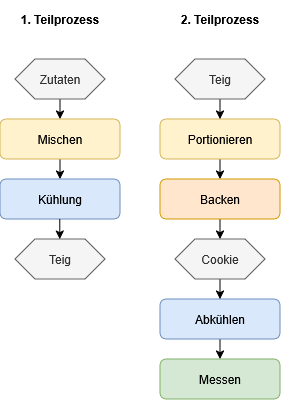
\includegraphics[width=\linewidth]{figures/prozess.png}
%     \caption{.}
%     \label{fig:prozess}
% \end{figure}
% Dann überlegst du pro Schritt, welche messbaren Merkmale entstehen oder beeinflusst werden.
% Beispiel:
% Prozessschritt	Mögliche Zielgröße
% Teig herstellen	Teigkonsistenz, Teigklebrigkeit, Teigtemperatur
% Portionieren	Rohteiggewicht, Rohteigdurchmesser
% Backen	Durchmesserzunahme, Höhenänderung, Bräunung
% Abkühlen	Endhöhe, Enddurchmesser, Festigkeit
% Lagerung	Feuchteverlust, Härtezunahme


\paragraph{Einfluss- und Störgrößen}

Zur Sammlung der Einfluss- und Störgrößen wird ein Ursache-Wirkungs-Diagramm \cite{Schu13} erstellt.
Bei der Erstellung des Diagramms werden alle Wirkungen auf ein Ziel identifiziert.
Die Wirkungen dienen zur Ableitung der Einfluss- und Störgrößen.
Das Ziel dieser Arbeit ist die Herstellung guter Cookies.
Die Hauptwirkungen auf das Ziel sind Material, Umwelt, Methoden, Maschine, Messung und Mensch.
Alle Nebenwirkungen sind in der Abbildung \ref{fig:ursache_wirkung} zu sehen.

\begin{figure}
    \centering
    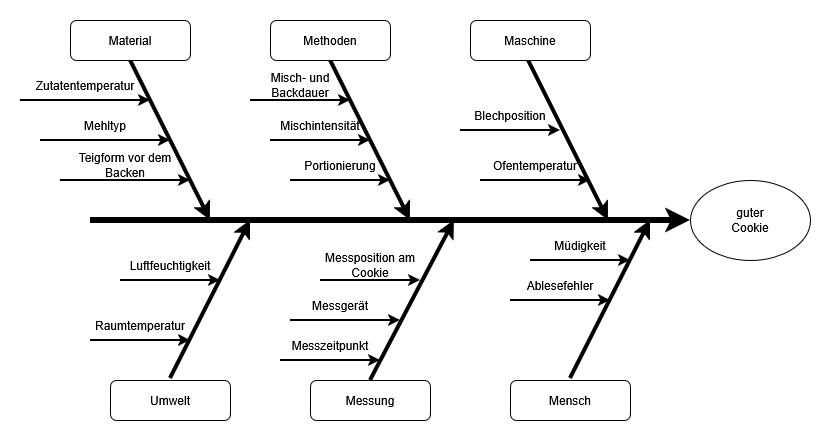
\includegraphics[width=\linewidth]{figures/ursachen-wirkungs-diagramm.drawio.png}
    \caption{Ursache-Wirkungs-Diagramm für gute Cookies.}
    \label{fig:ursache_wirkung}
\end{figure}

% \paragraph{P-Diagramm}

% Aus den gesammelten Größen lässt sich nun das Parameterdiagramm \cite{Sieb26} erstellen.
% Es teilt die Größen, die auf den Prozess wirken, in Signalgrößen, Steuergrößen, Störgrößen, Qualitätsmerkmale (hier Zielgrößen) und Error States.
% Die Abbildung \ref{fig:p_diagramm} zeigen die finale Einteilung der Größen.


\paragraph{Vorversuch}
Ein Vorversuch brachte wichtige Erkenntnisse. 
So wurden im Vorversuch Stückchen einer weißen Tafel Schokolade und Cranberries für die Cookies verwendet.
Die unterschiedlich großen Schokoladenstückchen und Cranberries führten zu starken variierenden Cookie-Formen.
Die Cookies aus dem Vorversuch sind in Abbildung \ref{fig:vorversuch} im Anhang \ref{ch:appendix_c} zu sehen.
Im Experiment werden deshalb Schokoladentropfen (SchokoTro) verwendet.
Diese sind maschinell gefertig und deutlich konsistenter in ihrer Größe.

Der Vorversuch nutzte zwei Extreme des Faktorraums.
Einen Teig mit 0\,\% Vollkornmehl, minimaler Zucker- und Buttermenge und ein Teig mit maximaler Zucker- und Buttermenge mit 0\,\% Vollkornmehl.
Dabei zeigten sich deutliche Unterschiede im Durchmesser und der Höhe der Cookies.
Es zeigte sich zudem, dass der Messzeitpunkt für den Durchmesser nach dem Backen nicht relevant ist.
Bei der Höhe sind 30 Minuten nach der Entnahme aus dem Ofen keine Änderungen messbar.
\chapter{Auswahl der Faktoren und Faktorstufen}\label{ch:studiendesign}

\paragraph{Feinbewertung und Festlegung der Zielgrößen}
Analyse der Zielgrößenabhängigkeiten (nicht gegeben - eine Zielgröße)
Festlegung der Messmethode und Messbereich (Messprozessfähigkeit muss geprüft und nachgewiesen werden)

\paragraph{Festlegung von Faktoren}
Butter und Zucker, da diese Faktoren die größten Schwankungen in den Rezepten aufweisen.
Vollkornmehl, um Erkenntnisse für gesündere Cookies zu erzeugen.

Vollkornmehl beeinflusst die Viskosität des Teiges stark.

\paragraph{Festlegung der Anzahl der Faktorstufen}
2 Stufen, um Komplexität gering zu halten
Erste Versuche in dem Feld
\paragraph{Festlegung der Werte der Faktorstufen}
Relativ großer Abstand - Risiko der Nicht-Linearität wird eingegangen.
\chapter{Versuchsplan und Durchführung}\label{ch:versuch}

% Versuchsplan
\paragraph{Der Versuchsplan (VP)} wird in der Software MiniTab \cite{minitab2026homepage} erstellt und analysiert.
Im VP sind drei Replikationen vorgesehen.
Jede Replikation wird in einem Block erfasst.
Damit werden die Streuung durch Störgrößen aus der Umwelt (Luftfeuchtigkeit, Raumtemperatur und Kühlschranktemperatur) minimiert.
Zusätzlich werden zwei Zentralpunkt pro Block vorgesehen.
Diese sollen eine spätere Prüfung auf Nichtlinearität des Modells ermöglichen.

Um schwankende Ofentemperaturen während des Backvorgangs zu vereinheitlichen, werden die Teige aller Faktorstufenkombinationen (FSK) gleichzeitig gebacken.
Damit fällt die Störgröße Blechposition mehr ins Gewicht.
Deshalb werden die Positionen in der ersten Replikation randomisiert.
Die Blechpositionen werden wie in Abbildung \ref{fig:positionen_rot} durchnummeriert.
Zudem bilden die Positionen drei Reihen (vorne, Mitte, hinten).
In der ersten Replikation ist die zufällige Durchlaufnummer gleichzeitig die Blechposition.
Für die weiteren Replikationen werden die Positionen für eine FSK systematisch rotiert.
Über die Position werden die Durchlaufnummern für die zweite und dritte Replikation definiert.
Die Rotationen sind durch rote Pfeile in der Abbildung \ref{fig:positionen_rot} dargestellt.
Mit der Rotation wird sichergestellt, dass jede FSK einmal in jeder Reihe war.
Einzig die Position 4 wird dabei nicht mitrotiert.
Auf ihr liegt immer eine FKS für den Zentralpunkt, der so unter konstanten Randbedingungen liegt.
Der entstandene Versuchsplan mit Durchlaufsnumern ist im Anhang \ref{ch:appendix_versuch} zu finden.

\begin{figure}
    \centering
    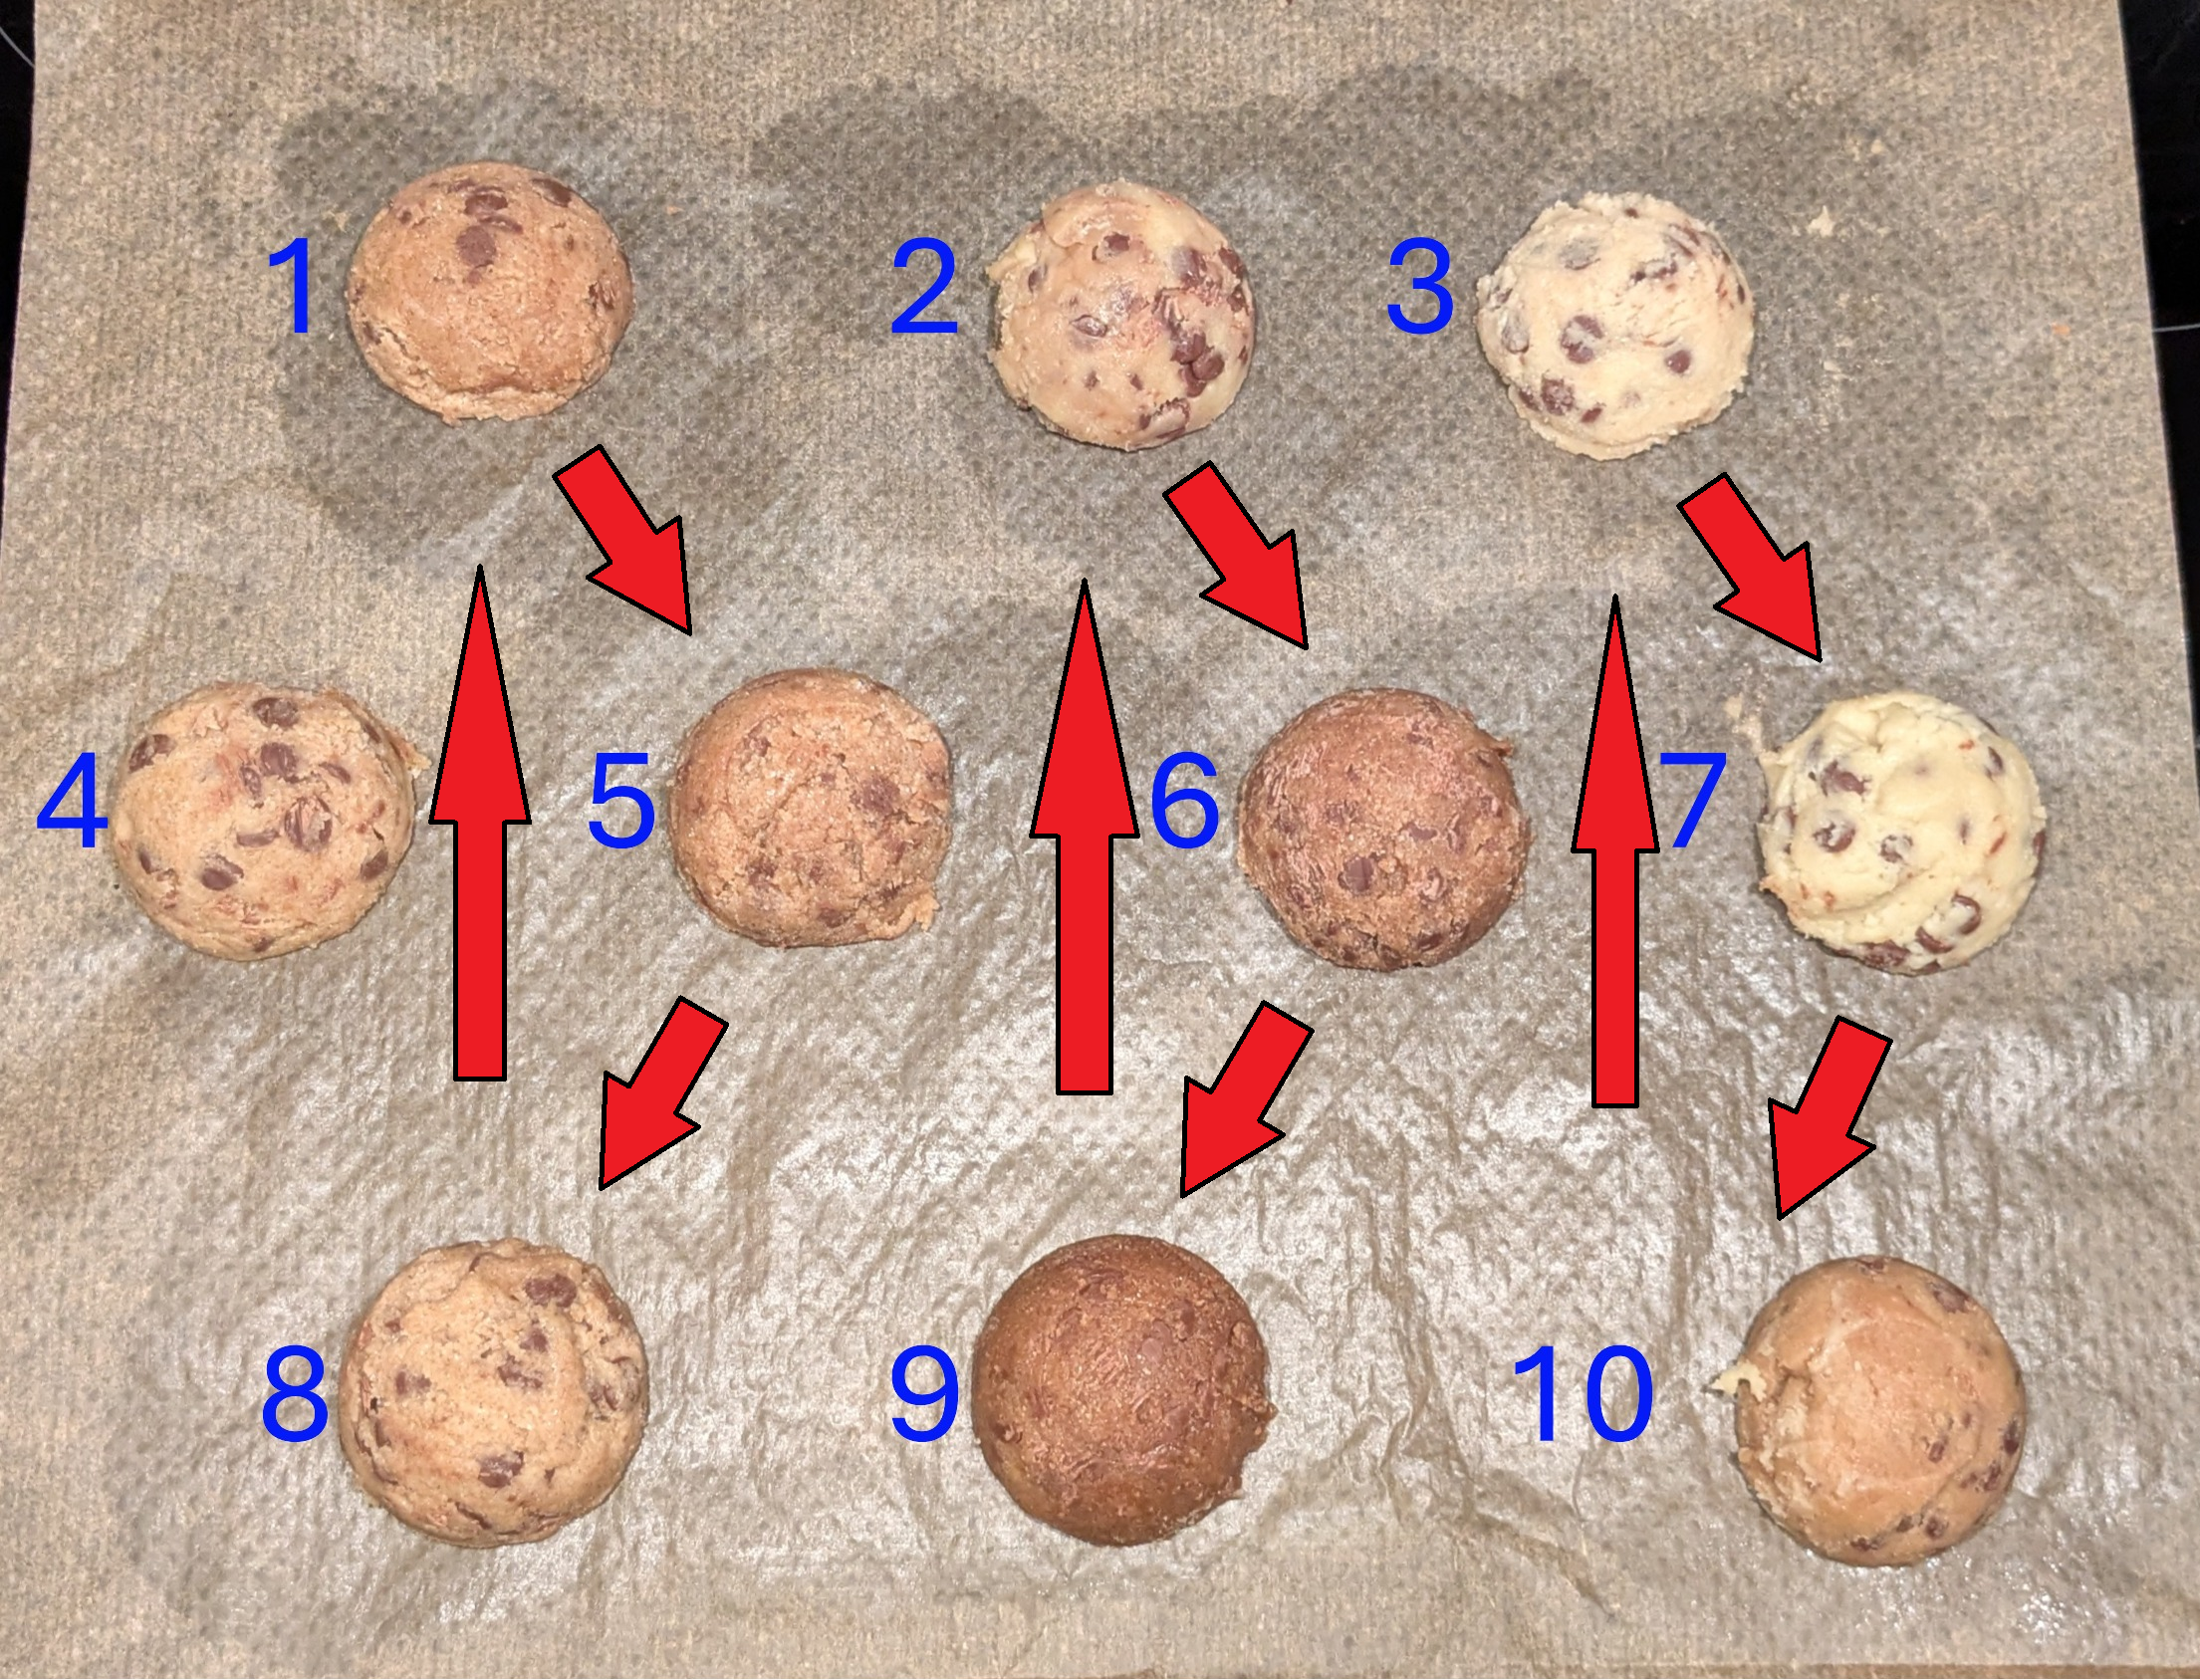
\includegraphics[width=0.7\linewidth]{figures/positionen_rot.png}
    \caption{Positionen auf dem Backblech in blau und die Rotation pro Replikation in rot.}
    \label{fig:positionen_rot}
\end{figure}

% Ablauf
\paragraph{Der Ablauf} einer Replikation wird in zwei Teilprozesse unterteilt (siehe Abbildung \ref{fig:prozess}).
Der Erste ist die Zubereitung der Teige für alle neun FSK, der Zweite das Backen und Messen der Cookies.
Dieser Ablauf wird für das Experiment drei mal durchgeführt.

\begin{figure}
    \centering
    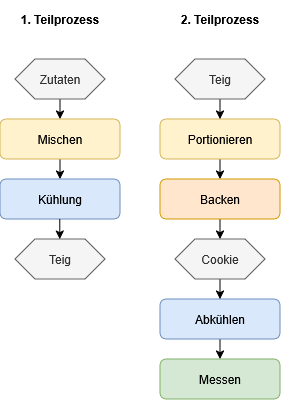
\includegraphics[width=0.4\linewidth]{figures/prozess.png}
    \caption{Prozess der Cookie-Herstellung mit zwei Teilprozessen. Links die Zubereitung des Teigs, rechts der Back- und Messvorgang.}
    \label{fig:prozess}
\end{figure}

Am Anfang einer Replikation werden alle Zutaten bereitgestellt.
Die Zutaten werden entsprechend der Prozessschritte in der Tabelle \ref{table:zubereitung_zugaben} zum Teig gegeben.
Diese Tabelle enthält auch die Temperaturen der Zutaten und das Messmittel um die Menge zu bestimmen.
Die Tabelle \ref{table:zubereitung_prozess} zeigt die Prozessschritte des Mischens.
Beide Tabellen zusammen haben eine fortlaufende Nummerierung der Prozessschritte.
Nach der Zubereitung wird der Teig in einen luftdichten Vorratsbehälter in den Kühlschrank gestellt.
Anschließend wird der Mischtopf gereinigt und getrocknet.
Dann wird mit dem Teig für die nächste FSK mit den gleichen Prozessschritten fortgefahren.
Zum Schluss des ersten Teilprozesses befinden sich neun Teige im Kühlschrank.
Dort ruhen sie für 22\,Stunden.

Am Folgetag wird zunächst der Ofen auf 175\,°C Umluft samt Backblech vorgeheizt.
Nach der Ruhezeit wird für jede FSK ein Teigrohling mit einem Eisportionierer (EP) geformt.
Der Teig wird dabei bündig zur Kante des EP abgezogen.
Anschließend wird der Teig, abzüglich des EP, gewogen.
Der Teigrohling wird auf einem Backpapier an der Blechposition entsprechend der Durchlaufnummer positioniert.
In der zweiten Replikation wird von der Durchlaufnummer zehn,
und in der dritten Replikation 20 von der Durchlaufnummer abgezogen, um auf die Position zu kommen.
Sind alle Teigrohlinge positioniert wird das Backblech aus dem Ofen entnommen und das Backpapier auf das Blech gezogen.
Das Blech wird im Ofen auf die mittlere Schiene geschoben.
Nach 11\,Minuten Backzeit wird das Blech entnommen und das Backpapier samt Cookies zum Abkühlen auf ein Gitter gezogen.
Nach 30\,Minuten Abkühlzeit werden die Cookies mit dem Messchieber vermessen.

\begin{table}
\centering
\caption{Prozessschritte der Zutatenzugaben für die Teigzubereitung}
\label{table:zubereitung_zugaben}
\begin{tabular}{|l|l|l|l|l|}
\hline
Schritt & Zutat               & Menge    & Temperatur  & Messmittel \\
\hline
1       & Butter              & nach VP     & Raum        & Küchenwaage \\
2       & Zucker              & nach VP     & Raum        & Küchenwaage \\
\hline
4       & Eier                & 2 (Größe M) & Kühlschrank & -- \\
\hline
6       & Mehl                & 280\,g      & Raum        & Küchenwaage \\
7       & Natron              & 3\,g        & Raum        & Feinwaage \\
8       & Salz                & 2\,g        & Raum        & Feinwaage \\
\hline
10      & Schokotropfen       & 100\,g      & Raum        & Küchenwaage \\
\hline
\end{tabular}
\end{table}

\begin{table}
\centering
\caption{Prozessschritte bei der Teigzubereitung}
\label{table:zubereitung_prozess}
\begin{tabular}{|l|l|l|l|l|}
\hline
Schritt & Operation & Dauer & Stufe & Gerät \\
\hline
3       & Mischen   & 40\,s & 4     & TM6 \\
5       & Mischen   & 15\,s & 4     & TM6 \\
9       & Mischen   & 20\,s & 4     & TM6 \\
11      & Mischen   & 20\,s & 3     & TM6 \\
\hline
\end{tabular}
\end{table}

% Aufwandabschätzung
\paragraph{Die Aufwandabschätzung} für das Experiment ergibt folgendes.
Die Zubereitung eines Teigs dauert circa 5\,Minuten, für neun FSK also 45\,Minuten.
Zusätzlich muss der Mischtopf neun mal gereinigt und getrocknet werden.
Das sind zusätzliche 45 Minuten, also 1,5\,Stunden für den ersten Teilprozess pro Replikation.
Während der Pause fällt kein Aufwand an.
Nur ein Teil der Kühlschrankkapazität wird für die Zeit gefordert.
Der zweite Teilprozess beinhaltet das Portionieren des Teigs zu Cookies.
Je Cookie-Portionierung wird mit anschließender Reinigung des Protionierers 1\,Minute geschätzt.
Dazu kommt das Backen im Ofen (11\,Minuten) mit anschließenden Abkühlen (30\,Minuten).
Für das Messen und übertragen der Werte werden 19\,Minuten eingeplant.
Pro Replikation werden 1\,Stunde für den zweiten Teilprozess und 2,5\,Stunden im Gesamten benötigt.
Der Aufwand für das Gesamte Experiment liegt damit bei 7,5\,Stunden verteilt auf 6 Tage.

% Vorversuch
\paragraph{Der Vorversuch} brachte wichtige Erkenntnisse. 
So wurden im Vorversuch Stückchen einer weißen Tafel Schokolade und Cranberries für die Cookies verwendet.
Die unterschiedlich großen Schokoladenstückchen und Cranberries führten zu starken variierenden Cookie-Formen.
Die Cookies aus dem Vorversuch sind in Abbildung \ref{fig:vorversuch} im Anhang \ref{ch:appendix_vorversuch} zu sehen.
Im Experiment werden deshalb Schokoladentropfen (SchokoTro) verwendet.
Diese sind maschinell gefertig und deutlich konsistenter in ihrer Größe.

Der Vorversuch nutzte zwei Extreme des Faktorraums.
Einen Teig mit 0\,\% Vollkornmehl, minimaler Zucker- und Buttermenge und ein Teig mit maximaler Zucker- und Buttermenge mit 0\,\% Vollkornmehl.
Dabei zeigten sich deutliche Unterschiede im Durchmesser und der Höhe der Cookies.
Es zeigte sich zudem, dass der Messzeitpunkt für den Durchmesser nach dem Backen nicht relevant ist.
Bei der Höhe sind 30 Minuten nach der Entnahme aus dem Ofen keine Änderungen messbar.

% ToDo
%Bestätigungsversuche ?! - Teig irgendwo im Raum, durch Formel berechnet
% Schritt 6: Auswertung
% - Effekte ermitteln, Signifikanz prüfen (Modellreduzierung!), R2-Werte; dabei
% Datenqualität prüfen (z. B. echte Ausreißer dürfen nicht ausgewertet werden!
% Einzelversuche wiederholen, neue Reduzierung)
% - Überprüfung der Modellvoraussetzungen nach jeder Modellreduzierung
% - Regressionsgleichung aufstellen, graphische Darstellung
\chapter{Ergebnisse}\label{ch:ergebnisse}

% 1. Analyse des vollständigen Modells und erste Diagnostik der Residuen
% Anhand der Varianzanalyse der Effekte wird abgeschätzt, welche Faktoren aufgrund des geringen Effekts kaum signifikant
% resp. für die Praxis nicht relevant sind. Eine erste graphische Residuendiagnostik wird durchgeführt, um grobe Abweichungen
% früh erkennen zu können.
\paragraph{Die Analyse des vollständigen Modells} zeigt das Modell ist klar signifikant ($p \le 0,001$).
Der R²-Wert (98,35\,\%) und der korrigierte R²-Wert (97,49\,\%) liegen nahe beieinander und nahe 100\,\%.
Das spricht für ein gutes Modell. % (siehe Abbildung \ref{fig:modell_gesamt}).
Alle drei Haupteffekte sind klar signifikant ($p \le 0,001$).
Die Zuckermenge wirkt sich am stärksten und positiv auf den Durchmesser aus ($13,542$),
gefolgt vom Anteil an Vollkornmehl ($-9,292$) mit einen negativen Effekt.
Die Buttermenge erzielt ebenfalls eine positiv Effekt ($8,292$) auf den Durchmesser.
Bei den Wechselwirkungen sind nur \emph{Butter*Zucker} und \emph{Zucker*Vollkornmehl} signifikant ($p \le 0,05$).
Die 2FWW \emph{Butter*Zucker} erreicht einen p-Wert von $0,032$ und hat mit $1,292$ nur einen geringen Effekt im Vergleich zu den Haupteffekten.
\emph{Zucker*Vollkornmehl} wirkt sich im gleichen Maß negativ auf den Durchmesser aus ($-1,292$) mit dem gleichen p-Wert wie \emph{Butter*Zucker}.

Die Krümmung zeigt Signifikanz ($p \le 0,05$) mit einem p-Wert von $0,033$.
Der Zentralpunkt ist mit den gleichem p-Wert signifikant.
Das deutet darauf hin, dass mindestens ein Faktor im Modell einen nicht-linearen Einfluss hat.
Der experimentelle Zentralpunkt liegt $1,438$ Einheiten unter dem errechneten Zentralpunkt ($71,771$) des Modells.
Bei den Blöcken zeigt Block 1 klare Signifikanz ($p \le 0,001$), während Block 2 mit einem p-Wert von $0,744$ nicht signifikant ist.
Die Blockbildung im Gesamten erreicht aber einen p-Wert von $0,000$.
Die Abbildung \ref{fig:analyse_gesamt} zeigt die relevanten Diagramme der Analyse.
Die Ergebnisse dazu sind im Anhang \ref{ch:appendix_ergebnisse} zu finden.

Die Regressionsgleichung für das vollständige Modell mit kodierten Einheiten ist wie folgt:

\begin{equation} \label{eq:modell_gesamt}
\begin{split}
\text{Durchsch\_Durchmesser} = & 71,771 - 1,583 \cdot \text{Block\_1} + 0,117 \cdot \text{Block\_2}  \\
    & + 4,146 \cdot \text{Butter} + 6,771 \cdot \text{Zucker} - 4,646 \cdot \text{Vollkornmehl} \  \\
    & + 0,646 \cdot (\text{Butter}\cdot\text{Zucker}) - 0,521 \cdot (\text{Butter}\cdot\text{Vollkornmehl})  \\
    & - 0,646 \cdot (\text{Zucker}\cdot\text{Vollkornmehl}) \\
    & + 0,312 \cdot (\text{Butter}\cdot\text{Zucker}\cdot\text{Vollkornmehl})  \\
    & - 1,438 \cdot \text{ZtrPkt}
\end{split}
\end{equation}

\begin{figure}
    \centering
\begin{subfigure}{0.49\textwidth}
    \centering
    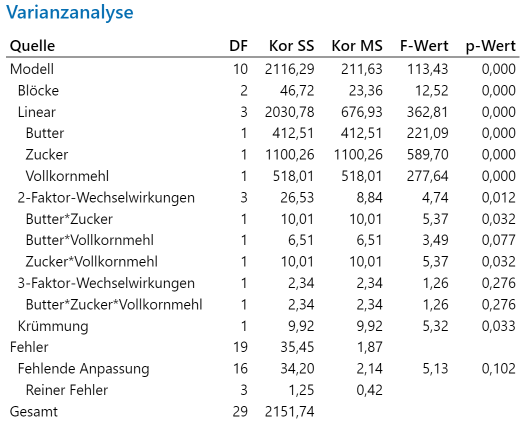
\includegraphics[width = \textwidth]{figures/varianzanalyse_gesamt.png}
    \caption{Varianzanalyse des vollständigen Modells}
    \label{fig:anova_gesamt}
\end{subfigure}\hfill
\begin{subfigure}{0.49\textwidth}
    \centering
    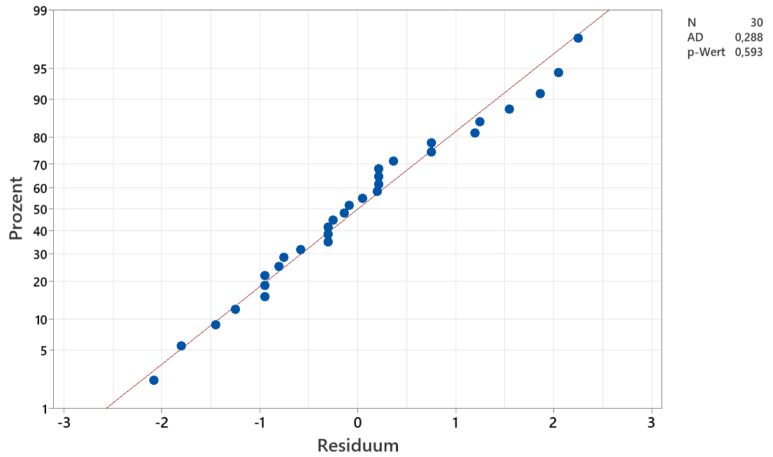
\includegraphics[width = \textwidth]{figures/wahrscheinlichkeitsnetz_gesamt.png}
    \caption{Wahrscheinlichkeitsnetz für die Normalverteilung}
    \label{fig:wahrscheinlichkeitsnetz_gesamt}
\end{subfigure}

\medskip

\begin{subfigure}{0.49\textwidth}
    \centering
    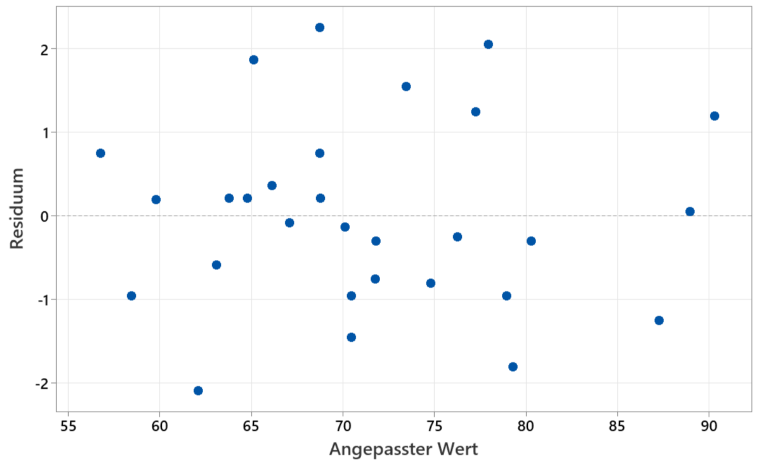
\includegraphics[width = \textwidth]{figures/residuen_anpassung_gesamt.png}
    \caption{Residuen in Abhängigkeit der Prognosewerte}
    \label{fig:residuen_anpassung_gesamt}
\end{subfigure}\hfill
\begin{subfigure}{0.49\textwidth}
    \centering
    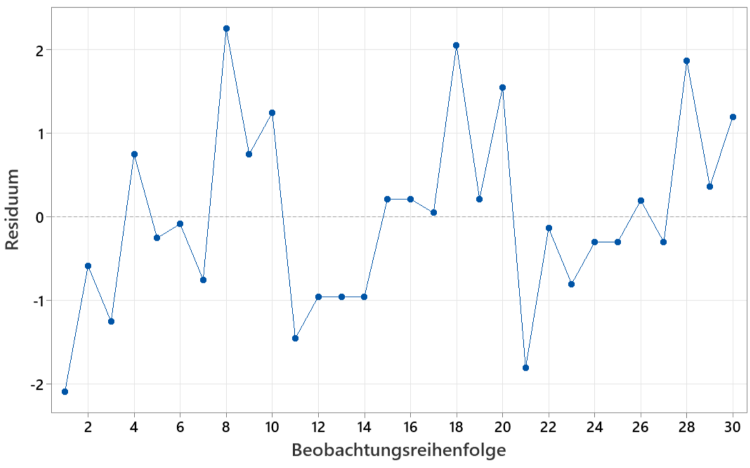
\includegraphics[width = \textwidth]{figures/residuen_reihenfolge_gesamt.png}
    \caption{Residuen in Abhängigkeit der Durchläufe}
    \label{fig:residuen_reihenfolge_gesamt}
\end{subfigure}

\caption{Analyse des vollständigen Modells}
\label{fig:analyse_gesamt}

\end{figure}

Die graphische Analyse der Residuen gibt keinen Hinweis auf eine Abweichungen der Normalverteilung (siehe Abbildung \ref{fig:wahrscheinlichkeitsnetz_gesamt}).
Zudem zeigt Abbildung \ref{fig:residuen_anpassung_gesamt}, dass die Residuen zufällig um die berechneten Prognosewerte gestreut sind.
Allerdings zeigt sich in der Analyse der Durchlaufnummern ein klar steigender Trend der Residuen innerhalb der Blöcke.
Die Blöcke haben die Durchlaufnummern 1-10, 11-20 und 21-30.
Dieser Trend ist auf die Blechposition zurück zu führen.
Die Positionen 1, 2 und 3 liegen hinten im Ofen während die Positionen 8, 9 und 10 vorne liegen.
Die Werte der Durchlaufnummer 1, 8, und 18 liegen dabei in einem kritischen Bereich.
Um diesen Trend auszugleichen wurden die Positionen randomisiert und strukturiert rotiert.
%Deshalb wird als nächstes mit der Modellreduzierung fortgefahren.

% 2. Vereinfachung des Modells
% Entfernen Sie nach und nach alle nicht signifikanten Terme aus dem Modell. Gehen Sie dabei sukzessive vor und entfernen
% Sie schrittweise immer den Effekt mit dem höchsten p-Wert, solange bis alle Effekte signifikant sind (Anmerkungen zur
% Hierarchie beachten). Zuerst Blöcke und Zentralpunkte entfernen (sofern nicht signifikant), dann weitere Terme.
\paragraph{Die Modellvereinfachung} beginnt mit der 3FWW \emph{Butter*Zucker*Vollkornmehl}, weil diese mit $0,276$ den größten p-Wert aufweist.
Zentralpunkt und die Blockbildung bleibt aufgrund der Signifikanz vorerst erhalten.
Durch die Vereinfachung weichen die Prognosen für die Durchlaufnummern 1 und 18 stärker ab.
Diese werden von MiniTab als \emph{ungewöhnliche Beobachtung} ausgewiesen und bewertet (siehe Abbildung \ref{fig:vereinfachung_1}).
Diese Beobachtungen sind auf die Blechpositionen zurückzuführen.
Der Fehler des Modells bleibt bei der \emph{Fehlenden Anpassung} allerdings nicht signifikant.
Auch die Residuen weichen nicht stark vom vorherigen Modell ab.

\begin{figure}
    \centering
    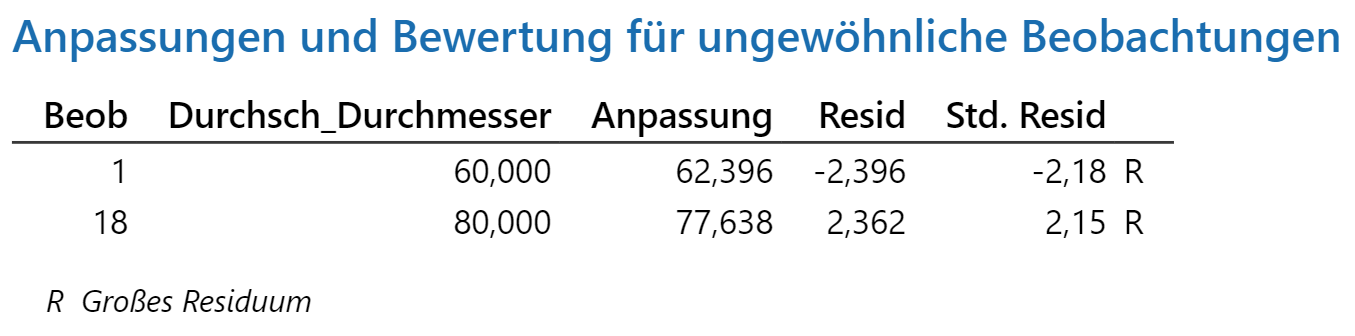
\includegraphics[width=\linewidth]{figures/anpassungen_vereinfachung_1.png}
    \caption{Ungewöhnliche Beobachtungen nach der ersten Vereinfachung}
    \label{fig:vereinfachung_1}
\end{figure}

Als nächstes wird die 2FWW \emph{Butter*Vollkornmehl} entfernt.
Diese weißt mit einem p-Wert von $0,078$ als nächste Wechselwirkungen keine Signifikanz auf.
Durch die Vereinfachung wird nur noch die Prognose für die Durchlaufnummern 1 als \emph{ungewöhnliche Beobachtung} ausgewiesen.
Die Residuen-Analyse ergibt keine Hinweise auf Änderungen in der Normalverteilung, Streuung oder in der Ablaufstruktur.
Damit sind für $p < 0,05$ alle nicht Signifikaten Faktoren und Wechselwirkungen entfernt.
Allerdings bleibt noch immer der Hinweis auf eine Krümmung mit dem p-Wert von $0,042$.

Darum wird für die weitere Vereinfachung das Signifikanzniveau von 5\,\% auf 1\,\% angehoben.
Damit wird als nächstes der Zentralpunkt aufgrund von fehlender Signifikanz aus dem Modell entfernt.
Für das neue Modell ergeben sich noch immer gute Werte für  R² (97,48\,\%) und R²(kor.) (96,68\,\%).
Allerdings wird ein Durchlauf mehr (1 und 20) als \emph{ungewöhnliche Beobachtung} ausgewiesen (siehe Abbildung \ref{fig:vereinfachung_3})
Die \emph{Fehlenden Anpassung} ist weiterhin nicht signifikant, genau wie nun auch die 2FWW \emph{Butter*Zucker} und \emph{Zucker*Vollkornmehl}.
Die Residuen zeigen weiterhin Normalverteilung mit zufälliger Streuung, und den Trend der Blechpositionen.

\begin{figure}
    \centering
    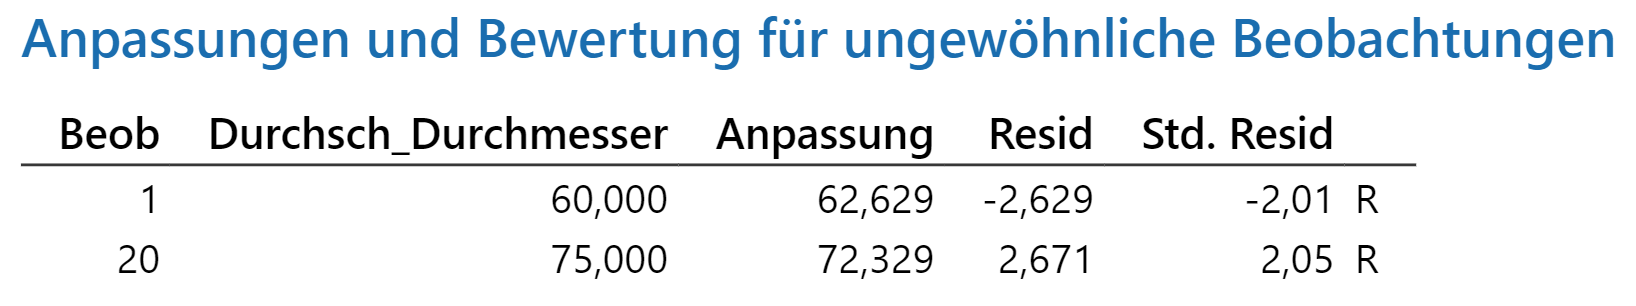
\includegraphics[width=\linewidth]{figures/anpassungen_vereinfachung_3.png}
    \caption{Ungewöhnliche Beobachtungen nach der dritten Vereinfachung}
    \label{fig:vereinfachung_3}
\end{figure}

Im nächsten Schritt wird die 2FWW \emph{Butter*Zucker} entfernt.
Dabei ergeben kaum Änderungen.
Nur der Durchlauf mit der Nummer 20 wird nichtmehr als \emph{ungewöhnliche Beobachtung} ausgewiesen.
Zudem steigt der p-Wert für die 2FWW \emph{Zucker*Vollkornmehl} auf $0,071$.
Diese Wechselwirkung wird im nächsten Schritt entfernt.
Das resultierende Modell aus der Vereinfachung ist final.

% 3. Diagnostik (des endgültigen Modells)
% Rechnen Sie das endgültige Modell erneut und führen Sie die dann finale Modelldiagnose durch. Prüfen Sie, ob die Residuen
% normalverteilt sind, ob sie zeitlich konstant sind und ob die Varianz der Residuen konstant ist. Prüfen Sie zudem den R2-Wert
% sowie den korrigierten R2-Wert (Zielwert > etwa 70 %)!
% Werfen Sie einen Blick auf den Lack of Fit und auf ungewöhnliche Beobachtungen (müssen ggf. einzelne Versuche neu
% durchgeführt werden, falls sich ein Ausreißer bestätigt)!
\paragraph{Das finale Modell} beinhaltet nur noch die drei Haupteffekt.
Diese sind alle klar signifikant.
Auch die Blockbildung ist weiterhin sehr signifikant mit einem p-Wert von $0,003$.
Der Block 1 hat einen p-Wert von $0,002$ während der Block 2 mit $0,799$ nichtmehr signifikant ist.
Der R²-Wert (96,55\,\%) und der korrigierte R²-Wert (95,83\,\%) liegen nahe beieinander und nahe 100\,\%.
Damit hat die Modellleistung zwar etwas abgenommen, ist aber mit sehr signifikanten Faktoren noch immer sehr gut.
Der Hinweis auf Krümmung ist nicht signifikant.
Es wird von Linearität ausgegangen.
Der p-Wert für die \emph{Fehlenden Anpassung} liegt bei $0,060$ und weist auf keine Signifikanz.
Dass der Wert sehr niedrig ist, kann unter anderem an den Ausreißern liegen.
Der Durchlauf mit der Nummer 9 wird nun als \emph{ungewöhnliche Beobachtung} ausgewiesen.
Bei Analyse der Residuen zeigt sich, dass es keine Hinweis gegen eine Normalverteilung gibt (siehe Abbildung \ref{fig:wahrscheinlichkeitsnetz_final}).
Die Residuen streuen relativ stark, sind aber zufällig um die Prognosewerte verteilt.
Der Trend der Blechpositionen ist noch erkennbar, nahm aber mit der Vereinfachung des Modells ab.

\begin{figure}
    \centering
\begin{subfigure}{0.47\textwidth}
    \centering
    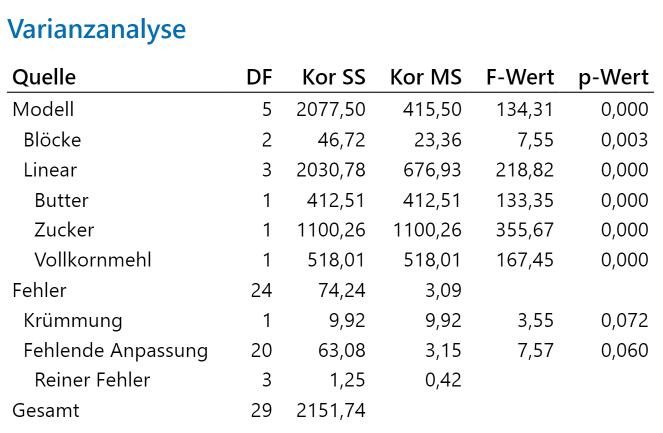
\includegraphics[width = \textwidth]{figures/varianzanalyse_final.png}
    \caption{Varianzanalyse des finalen Modells}
    \label{fig:anova_final}
\end{subfigure}\hfill
\begin{subfigure}{0.47\textwidth}
    \centering
    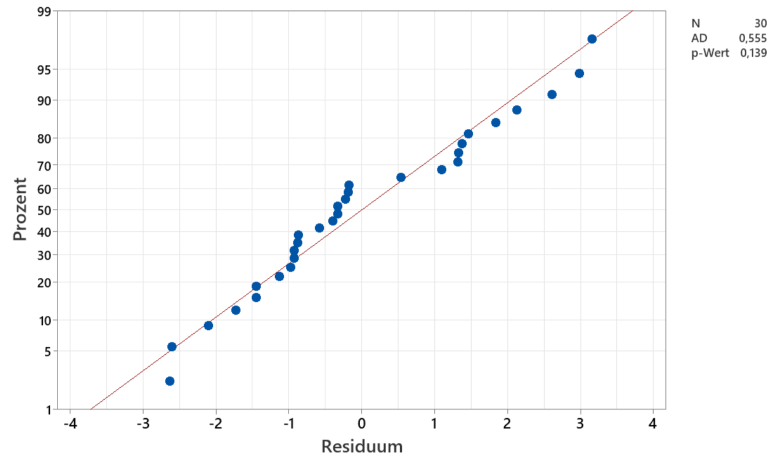
\includegraphics[width = \textwidth]{figures/wahrscheinlichkeitsnetz_final.png}
    \caption{Wahrscheinlichkeitsnetz für die Normalverteilung}
    \label{fig:wahrscheinlichkeitsnetz_final}
\end{subfigure}

\medskip

\begin{subfigure}{0.47\textwidth}
    \centering
    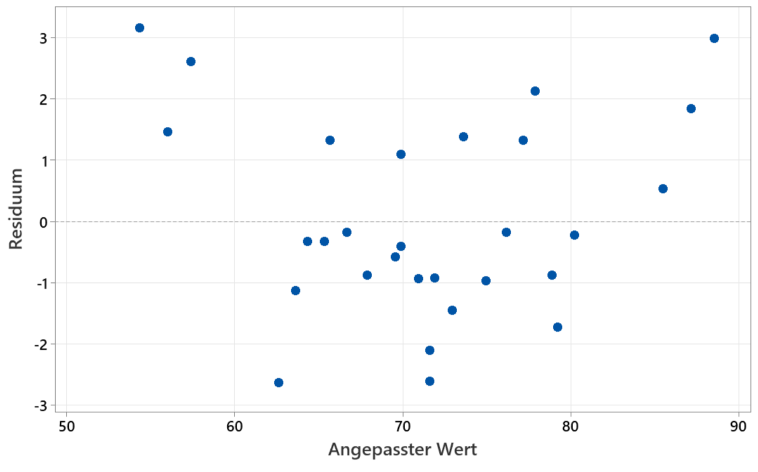
\includegraphics[width = \textwidth]{figures/residuen_anpassung_final.png}
    \caption{Residuen in Abhängigkeit der Prognosewerte}
    \label{fig:residuen_anpassung_final}
\end{subfigure}\hfill
\begin{subfigure}{0.47\textwidth}
    \centering
    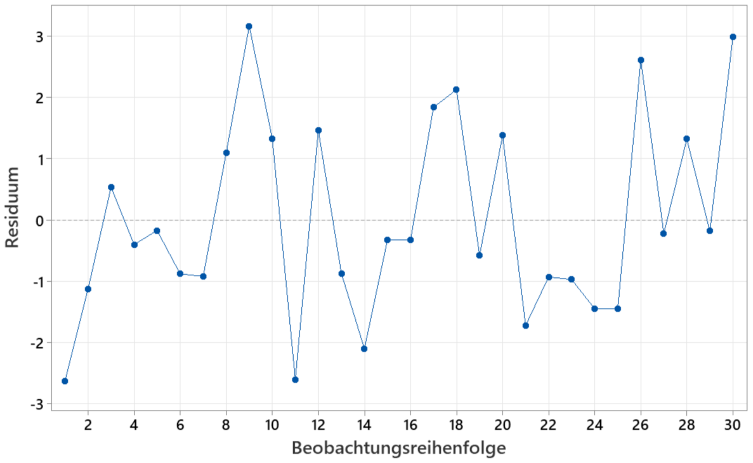
\includegraphics[width = \textwidth]{figures/residuen_reihenfolge_final.png}
    \caption{Residuen in Abhängigkeit der Durchläufe}
    \label{fig:residuen_reihenfolge_final}
\end{subfigure}

\caption{Analyse des finale Modells}
\label{fig:analyse_final}
\end{figure}

% NICHT MÖGLICH
% 4. Ermittlung der optimalen Einstellungen
% Erstellen Sie Wechselwirkungs- und Haupteffekt-Plots bzw. erstellen Sie Cube-Plots. Untersuchen Sie, wo Sie die optimale
% Einstellung finden und ob robuste Prozesseinstellungen vorhanden sind.
% Achtung: Nicht signifikante Effekte sind dabei – trotz graphischer Darstellbarkeit – nicht zu berücksichtigen.
Die Haupteffekt erzielen die gleichen Effekte wie im vollständigen Modell.
Mehr Zucker oder Butter führen zu größeren Durchmesser, wobei Zucker stärker wirkt.
Mit zunehmenden Vollkornmehlanteil sinkt der Durchmesser des Cookies hingegen.
Dies lässt sich nur für den Faktorraum gesichert sagen.
Die Abbildung \ref{fig:haupteffekte_diagramm} zeigt die Wirkungen der Haupteffekte im Faktorraum.
Eine Optimierung ist in der Arbeit nicht vorgesehen, da der optimale Durchmesser von der Vorliebe des Konsumenten abhängt.

% NICHT MÖGLICH
% 5. Ergebnisprognose
% Erstellen Sie auf Basis des endgültigen mathematischen Modells die Vorhersage für das optimale Ergebnis, indem Sie die
% Regressionsgleichung aufstellen und das Ergebnis berechnen.
% Achtung: Achten Sie beim mathematischen Modell auf die unterschiedlichen Koeffizienten für das codierte und das uncodierte
% Modell. Im Kurs wird nur das kodierte Modell verwendet!

% Die Ergebnisinterpretation erfolgt graphisch.
% Bei signifikanten Wechselwirkungen verwenden wir den Wechselwirkungsplots
% Die Wechselwirkungsplots untersuchen wir unter 2 Gesichtspunkten:
% - Welches sind die optimalen Einstellungen bezogen auf die Zielgröße?
% - Gibt es robuste Prozesseinstellungen?
% Bei signifikanten Haupteffekten verwenden wir den Haupteffektplot
% - Die Haupteffektplots untersuchen wir unter dem Gesichtspunkt:
% Was sind die optimalen Einstellungen?
% - Als weitere Möglichkeit können Sie den Cube Pot darstellen
% - Zur Darstellung der Zielgröße im gesamten Versuchsraum sind Kontur-und
% Antwortflächendiagramme sinnvoll

\begin{figure}
    \centering
    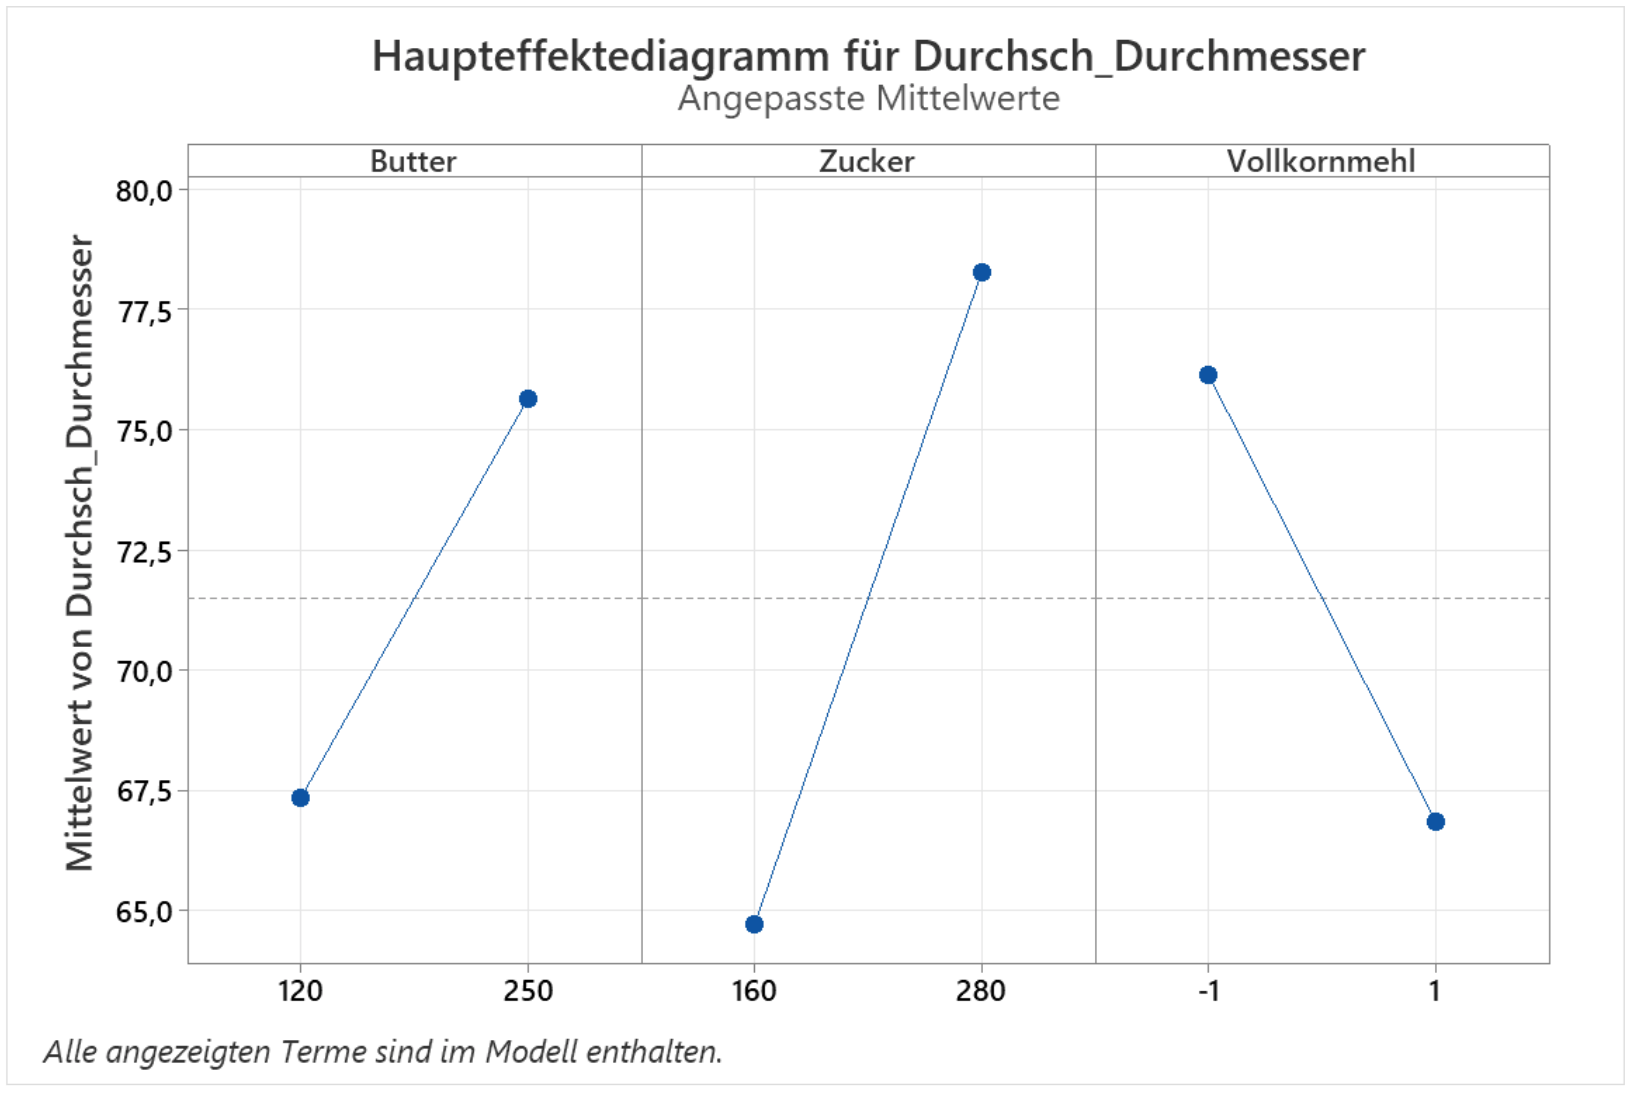
\includegraphics[width=0.7\linewidth]{figures/haupteffekte_diagramm.png}
    \caption{Haupteffekte und deren Wirkung auf den Durchmesser}
    \label{fig:haupteffekte_diagramm}
\end{figure}

Die Regressionsgleichung in kodierter Form für das finale Modell ist wie folgt:

\begin{equation} \label{eq:modell_final}
\begin{split}
\text{Durchsch\_Durchmesser} = & 71,483 - 1,583 \cdot \text{Block\_1} + 0,117 \cdot \text{Block\_2} \\
                               & + 4,146 \cdot \text{Butter} + 6,771 \cdot \text{Zucker} - 4,646 \cdot \text{Vollkornmehl}
\end{split}
\end{equation}
\chapter{Schlussfolgerung}\label{ch:schlussfolgerung}

\printbibliography[title={Literaturverzeichnis}]

\appendix  % Start appendix section (uses letters: A, B, C instead of 1, 2, 3)
\chapter{Rezepte} \label{ch:appendix_rezepte}
\vspace{-1.0\baselineskip}

Die sind die Rezepte mit den Mengenangaben. Dabei wurde Packpulver mit dem Faktor $0,75$ in Natron umgerechnet.
Zudem wurden sämtliche Zutaten, die als Füllung gedacht sind mit SchokoSt bezeichnet.
Zucker jeglicher Art (raffinierter, braun oder Vanillezucker) wurde zu Zucker hinzugezählt.
War bei den Zutaten von einem Eigelb die Rede wird dieses mit als $0,5$\,Eier gewertet.  
\begin{table}[h!]
\centering
\caption{Rezepte mit Mengenangabe der Zutaten (Teil 1: Basisteig)}
\label{table:rezepte_1}
\begin{tabular}{|l|r|r|r|r|}
\hline
Rezept & Mehl (g) & Butter (g) & Zucker (g) & Eier (Stk.) \\
\hline
R1     & 280      & 250        & 260        & 2,0         \\
R2     & 280      & 250        & 238        & 2,0         \\
R3     & 250      & 170        & 168        & 1,5         \\
R4     & 280      & 170        & 258        & 1,5         \\
R5     & 375      & 250        & 375        & 2,0         \\
R6     & 240      & 170        & 200        & 1,0         \\
R7     & 180      & 130        & 208        & 1,0         \\
R8     & 250      & 120        & 184        & 1,0         \\
\hline
\end{tabular}
\end{table}

\begin{table}[h!]
\centering
\caption{Rezepte mit Mengenangabe der Zutaten (Teil 2: Triebmittel und Schokost\"uckchen)}
\label{table:rezepte_2}
\begin{tabular}{|l|r|r|r|}
\hline
Rezept & Natron (g) & Salz (g) & SchokoSt (g) \\
\hline
R1     & 3,0        & 2,5      & 300          \\
R2     & 3,0        & 2,5      & 200          \\
R3     & 1,5        & 1,7      & 200          \\
R4     & 3,0        & 0,5      & 150          \\
R5     & 4,0        & 0,5      & 300          \\
R6     & 3,0        & 2,5      & 250          \\
R7     & 1,5        & 0,5      & 140          \\
R8     & 3,0        & 0,5      & 150          \\
\hline
\end{tabular}
\end{table}

% 1TL (gestr.) Salz entspricht 2,5 g
% 1TL Natron entspricht 3 g
% 1 Pck. Vanillezucker entspricht 8 g
% 1 TL Vanillezucker entspricht 4 g
% 1 Prise Salz entspricht 0,5 g
% Eier liegen meist bei 2 Stück
% Eier manchmal auch ein ganzen und ein Eigelb

% R1 : https://www.chefkoch.de/rezepte/2257651361176625/Subway-Cookies.html  
% R2 : https://www.chefkoch.de/rezepte/1378031243002711/American-Cookies-wie-bei-Subway.html  
% R3 : https://www.chefkoch.de/rezepte/470791140633601/Chewy-Chocolate-Chip-Cookies.html  
% R4 : https://www.chefkoch.de/rezepte/2601991408817771/American-Soft-Chocolate-Chip-Cookies.html  
% R5 : https://www.chefkoch.de/rezepte/614921161520963/World-s-best-Chocolate-Chip-Cookies.html  
% R6 : https://cookidoo.de/recipes/recipe/de-DE/r307943  
% R7 : https://cookidoo.de/recipes/recipe/de-DE/r47866    
% R8 : https://cookidoo.de/recipes/recipe/de-DE/r136546  


\begin{table}[H]
\centering
\caption{Links zu den Rezepten}
\label{table:rezepte_links}
\small
\begin{tabular}{|l|>{\RaggedRight\arraybackslash}p{0.78\textwidth}|}
\hline
Rezept & Link \\
\hline
R1     & \url{https://www.chefkoch.de/rezepte/2257651361176625/Subway-Cookies.html} \\
R2     & \url{https://www.chefkoch.de/rezepte/1378031243002711/American-Cookies-wie-bei-Subway.html} \\
R3     & \url{https://www.chefkoch.de/rezepte/470791140633601/Chewy-Chocolate-Chip-Cookies.html} \\
R4     & \url{https://www.chefkoch.de/rezepte/2601991408817771/American-Soft-Chocolate-Chip-Cookies.html} \\
R5     & \url{https://www.chefkoch.de/rezepte/614921161520963/World-s-best-Chocolate-Chip-Cookies.html} \\
R6     & \url{https://cookidoo.de/recipes/recipe/de-DE/r307943} \\
R7     & \url{https://cookidoo.de/recipes/recipe/de-DE/r47866} \\
R8     & \url{https://cookidoo.de/recipes/recipe/de-DE/r136546} \\
\hline
\end{tabular}
\end{table}



\chapter{Aufstellung der verwendeten Mess- und Prozessmittel} \label{ch:appendix_material}
\vspace{-1.0\baselineskip}
\begin{table}
\centering
\caption{Verwendete Messmittel}
\label{table:messmittel}
\begin{tabular}{|l|r|r|r|r|}
\hline
Messmittel        & Hersteller & Typ        & Auflösung & Beschreibung \\
\hline
Messschieber      & KRAFT      &            & 0,02mm    &               \\
Thermometer       &            &            && \\          
\hline
\end{tabular}
\end{table}

\begin{table}
\centering
\caption{Verwendete Prozessmittel}
\label{table:prozessmittel}
\begin{tabular}{|l|l|l|l|}
\hline
Prozessmittel     & Hersteller & Typ      & Beschreibung \\
Küchenwaage       & Tefal      &          &          \\
Feinwaage         &            &          &          \\
Thermomix         & Vorwerk    & TM6      &        \\
Vorratsbehälter   & IKEA       & IKEA 365+ Vorratsbehälter & mit luftdichten Kunstoffdeckel \\
Eisportionierer   & IKEA       & IDEALSIK & aus Edelstahl mit Doppellöffel   \\
\hline
\end{tabular}
\end{table}



\chapter{Cookies aus dem Vorversuch} \label{ch:appendix_vorversuch}
\vspace{-1.0\baselineskip}
\begin{figure}[H]
    \centering
    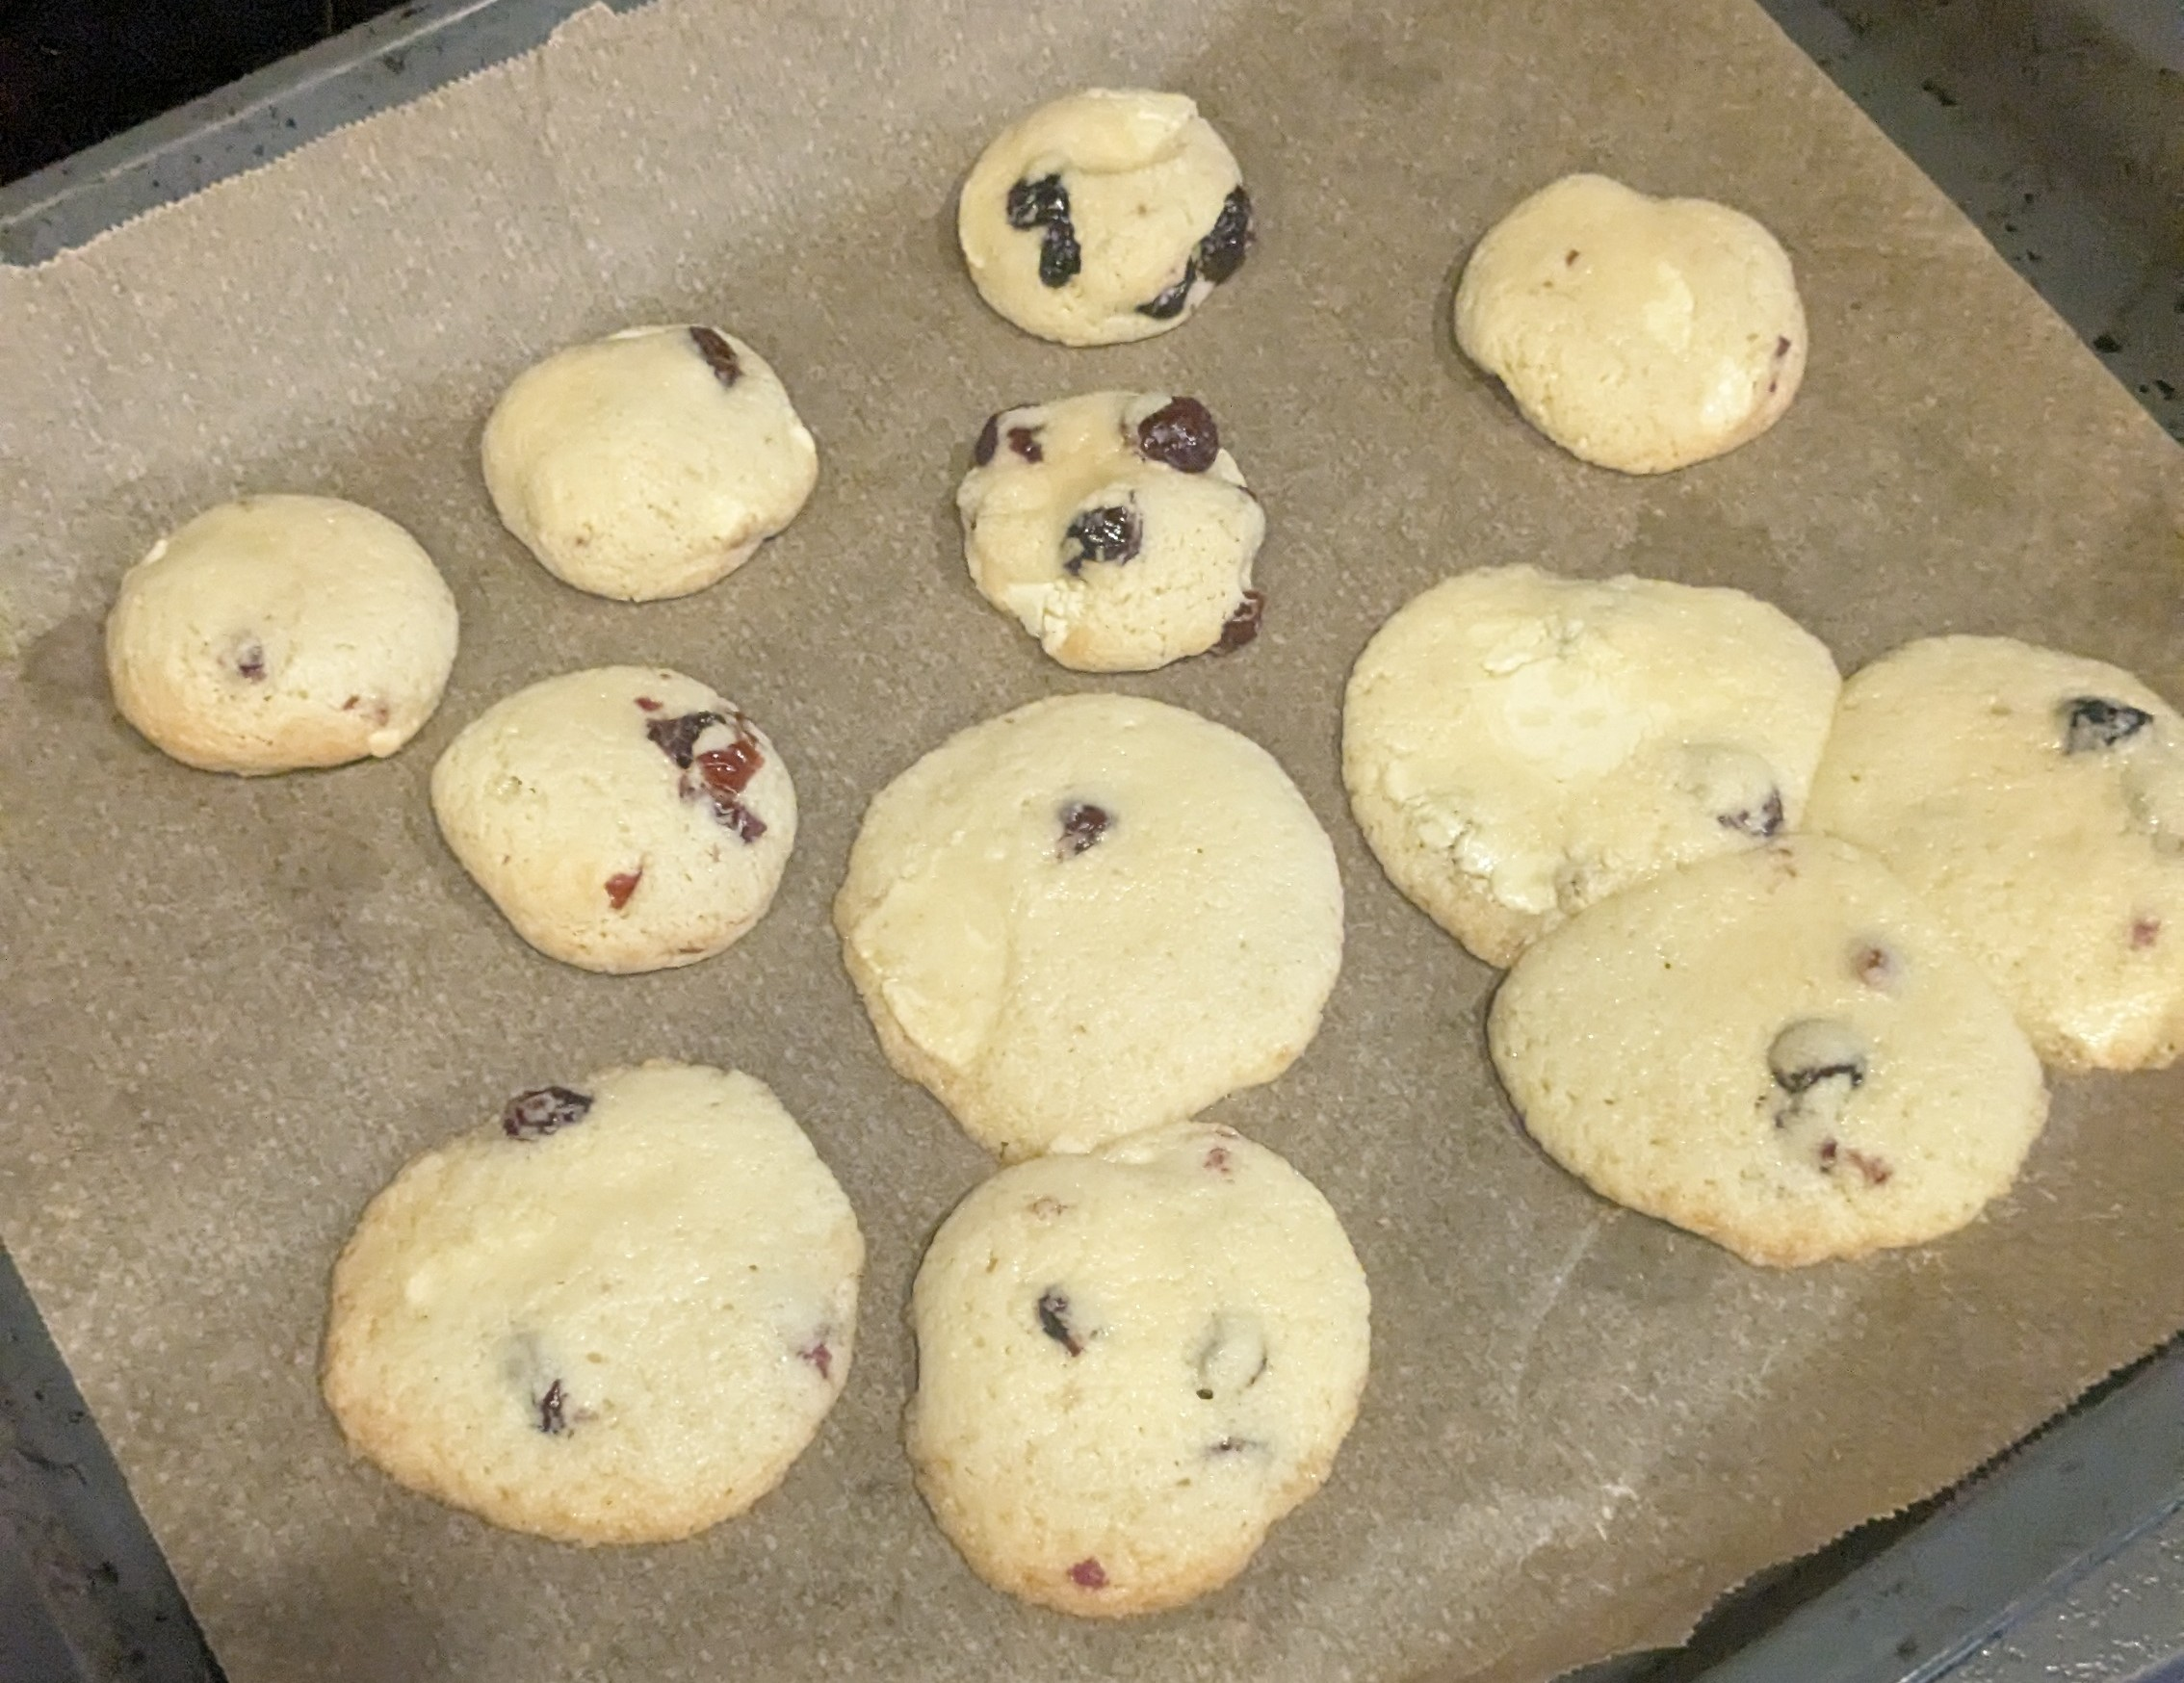
\includegraphics[width=\linewidth]{figures/vorversuch.jpg}
    \caption{Im Vorversuch mit unregelmäßigen Stücken von einer weißen Schokoladentafel und Cranberries ergaben sich variierende Cookie-Formen.}
    \label{fig:vorversuch}
\end{figure}

\chapter{Messmethoden} \label{ch:appendix_messung}
\vspace{-1.0\baselineskip}
\begin{figure}[H]
    \centering
    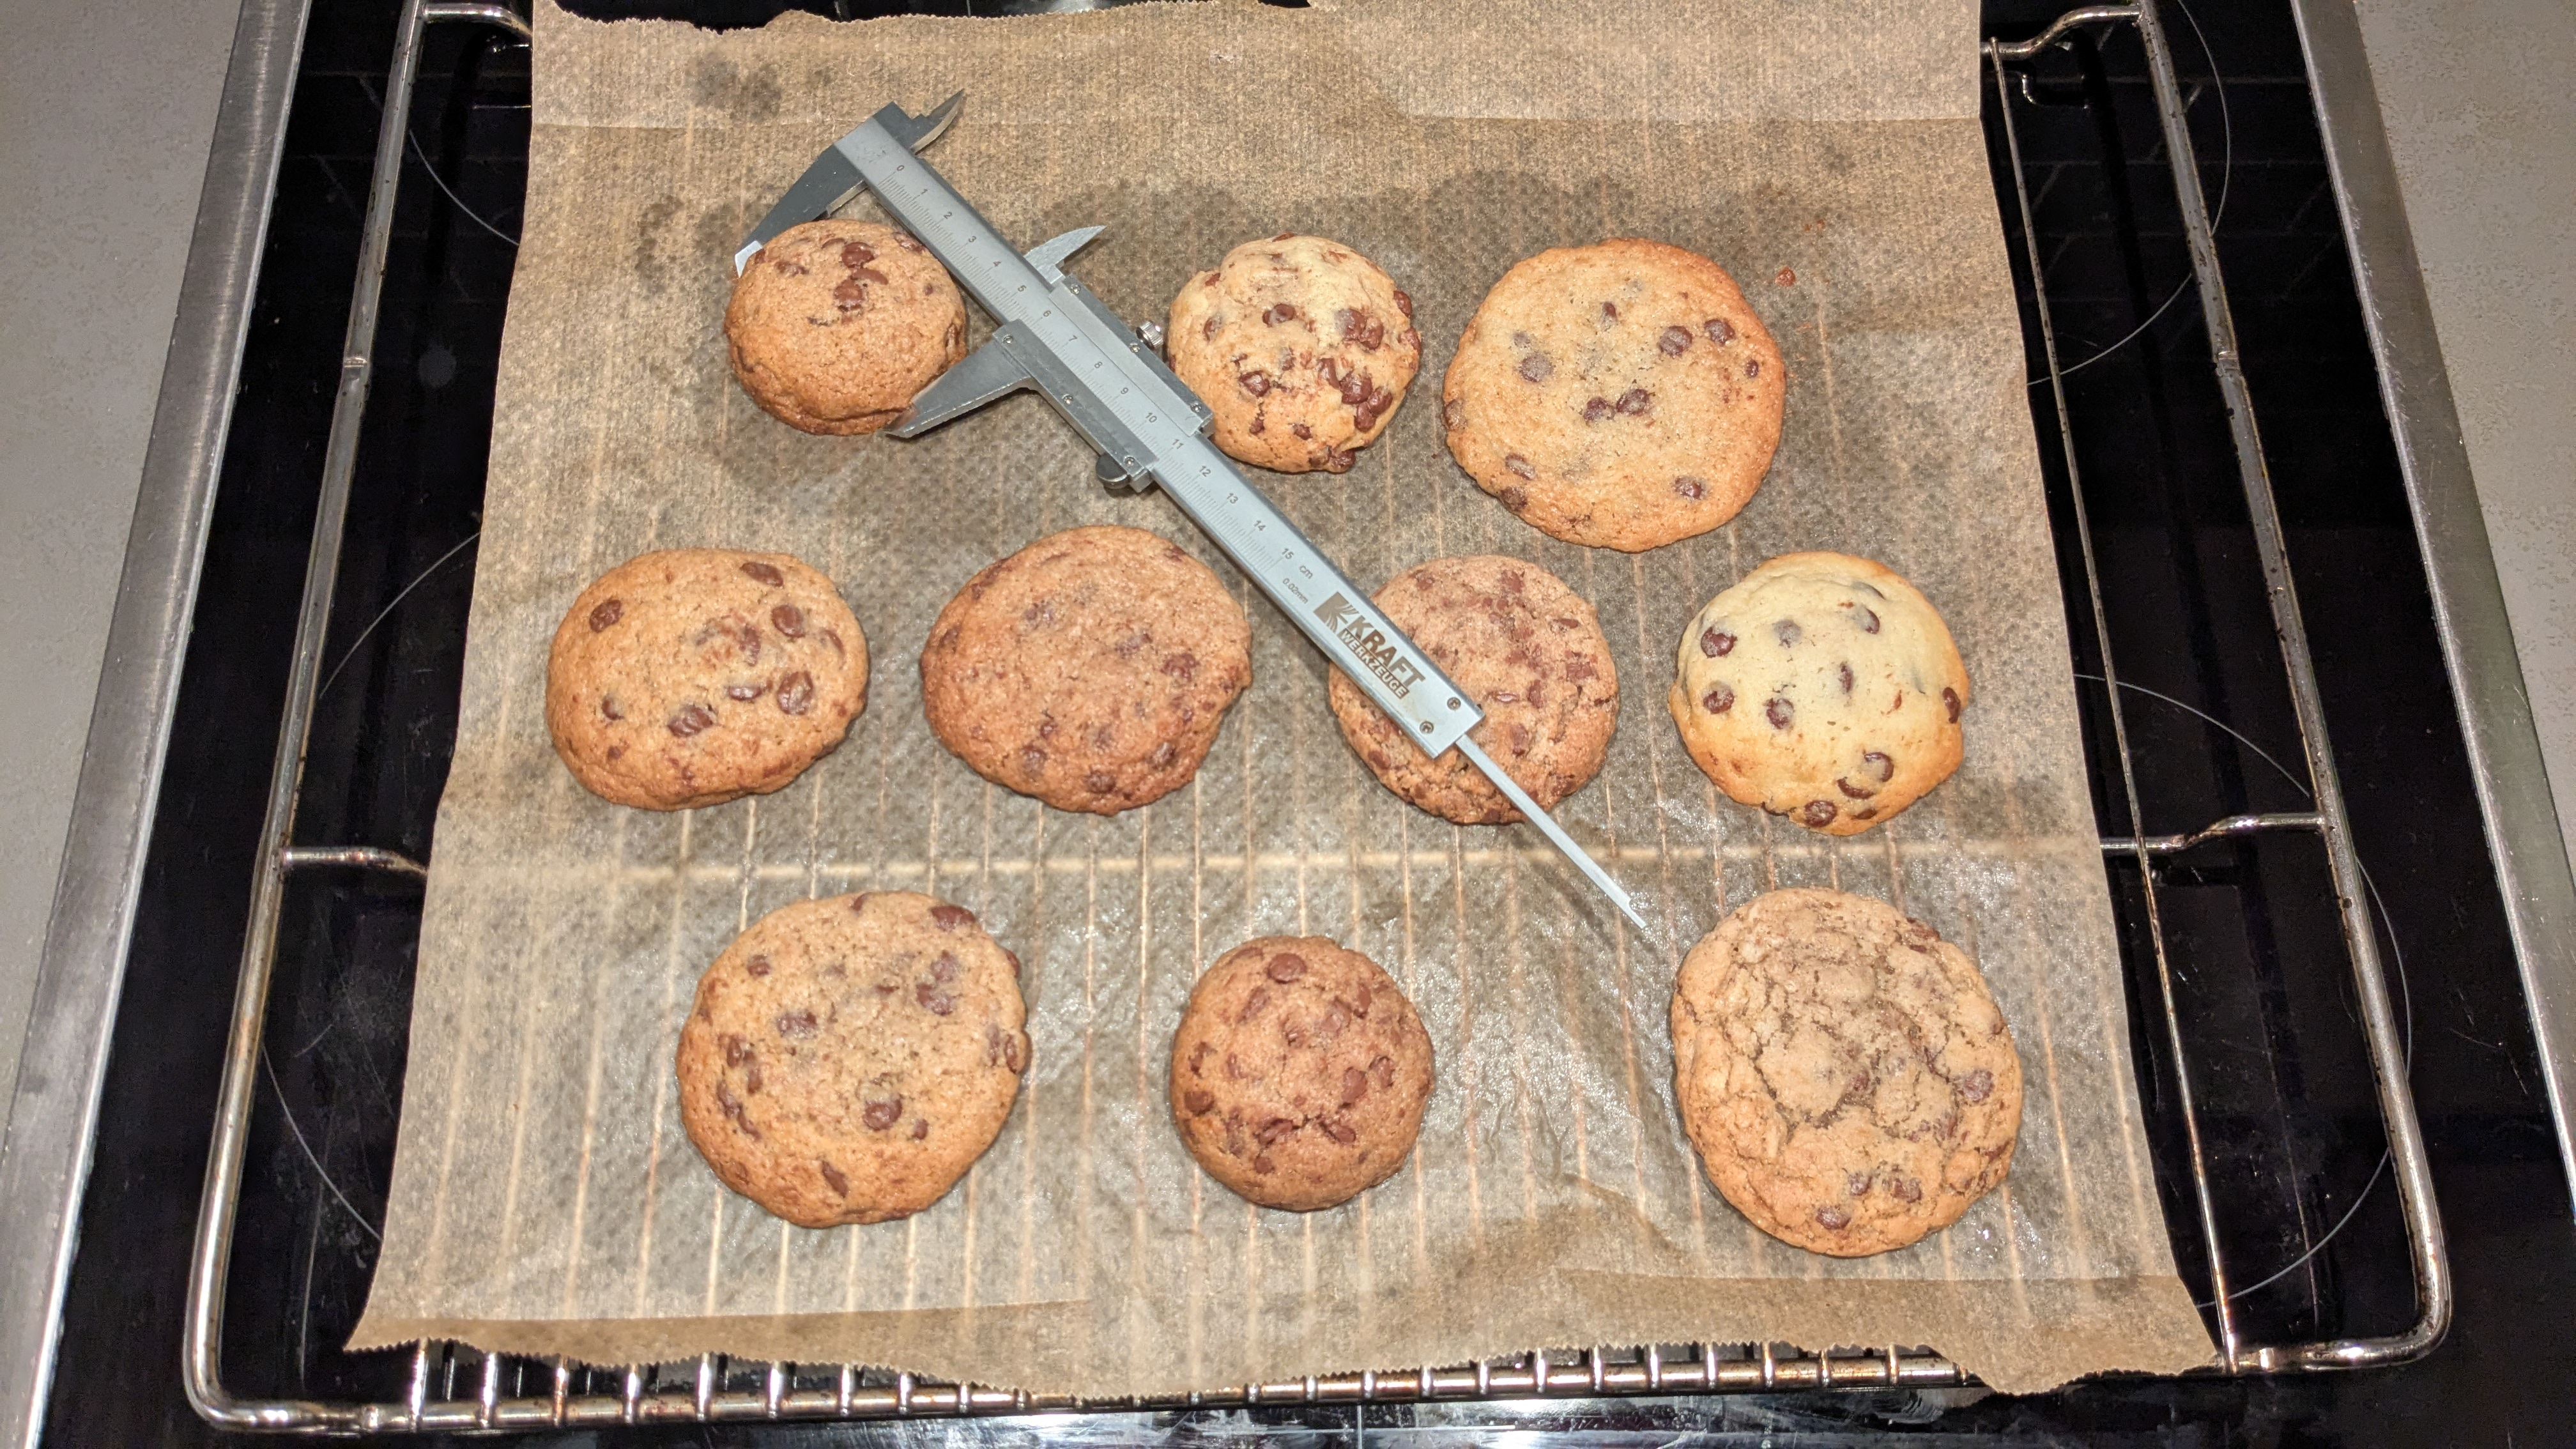
\includegraphics[width=\linewidth]{figures/messung_d1.jpg}
    \caption{Messung des ersten Durchmessers}
    \label{fig:messung_d1}
\end{figure}

\begin{figure}[H]
    \centering
    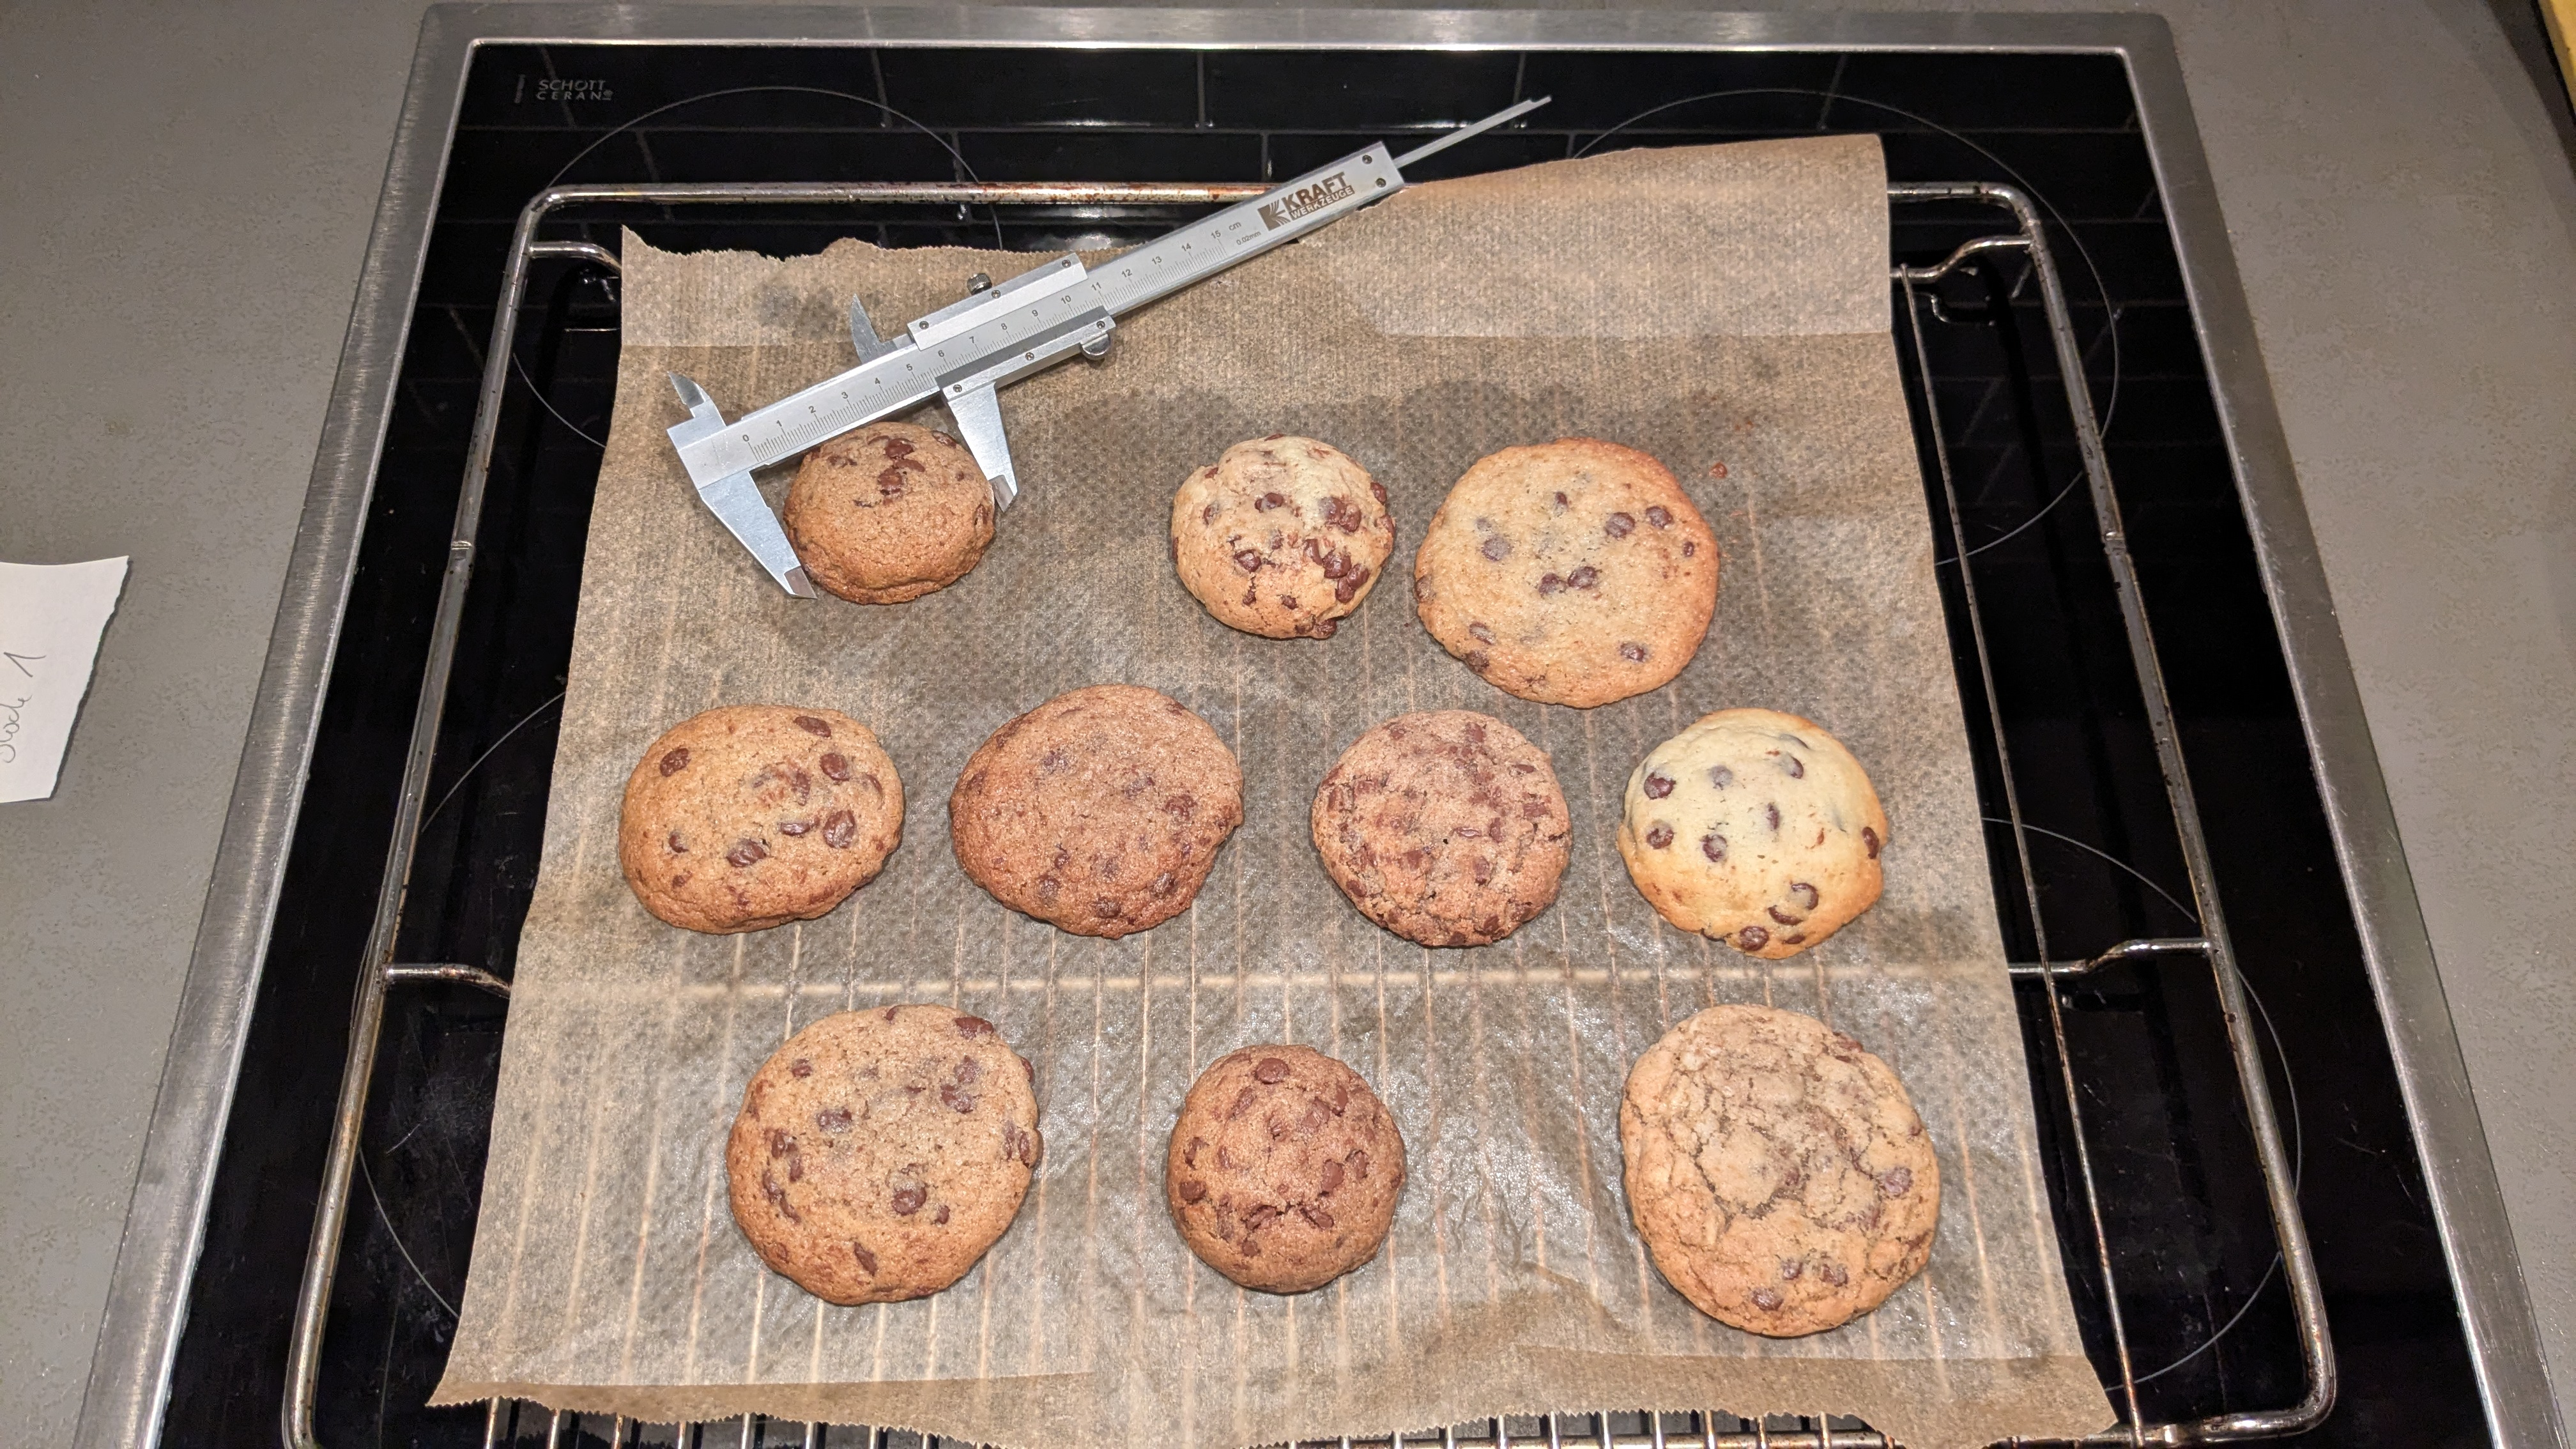
\includegraphics[width=\linewidth]{figures/messung_d2.jpg}
    \caption{Messung des zweiten Druchmessers}
    \label{fig:messung_d2}
\end{figure}

\begin{figure}[H]
    \centering
    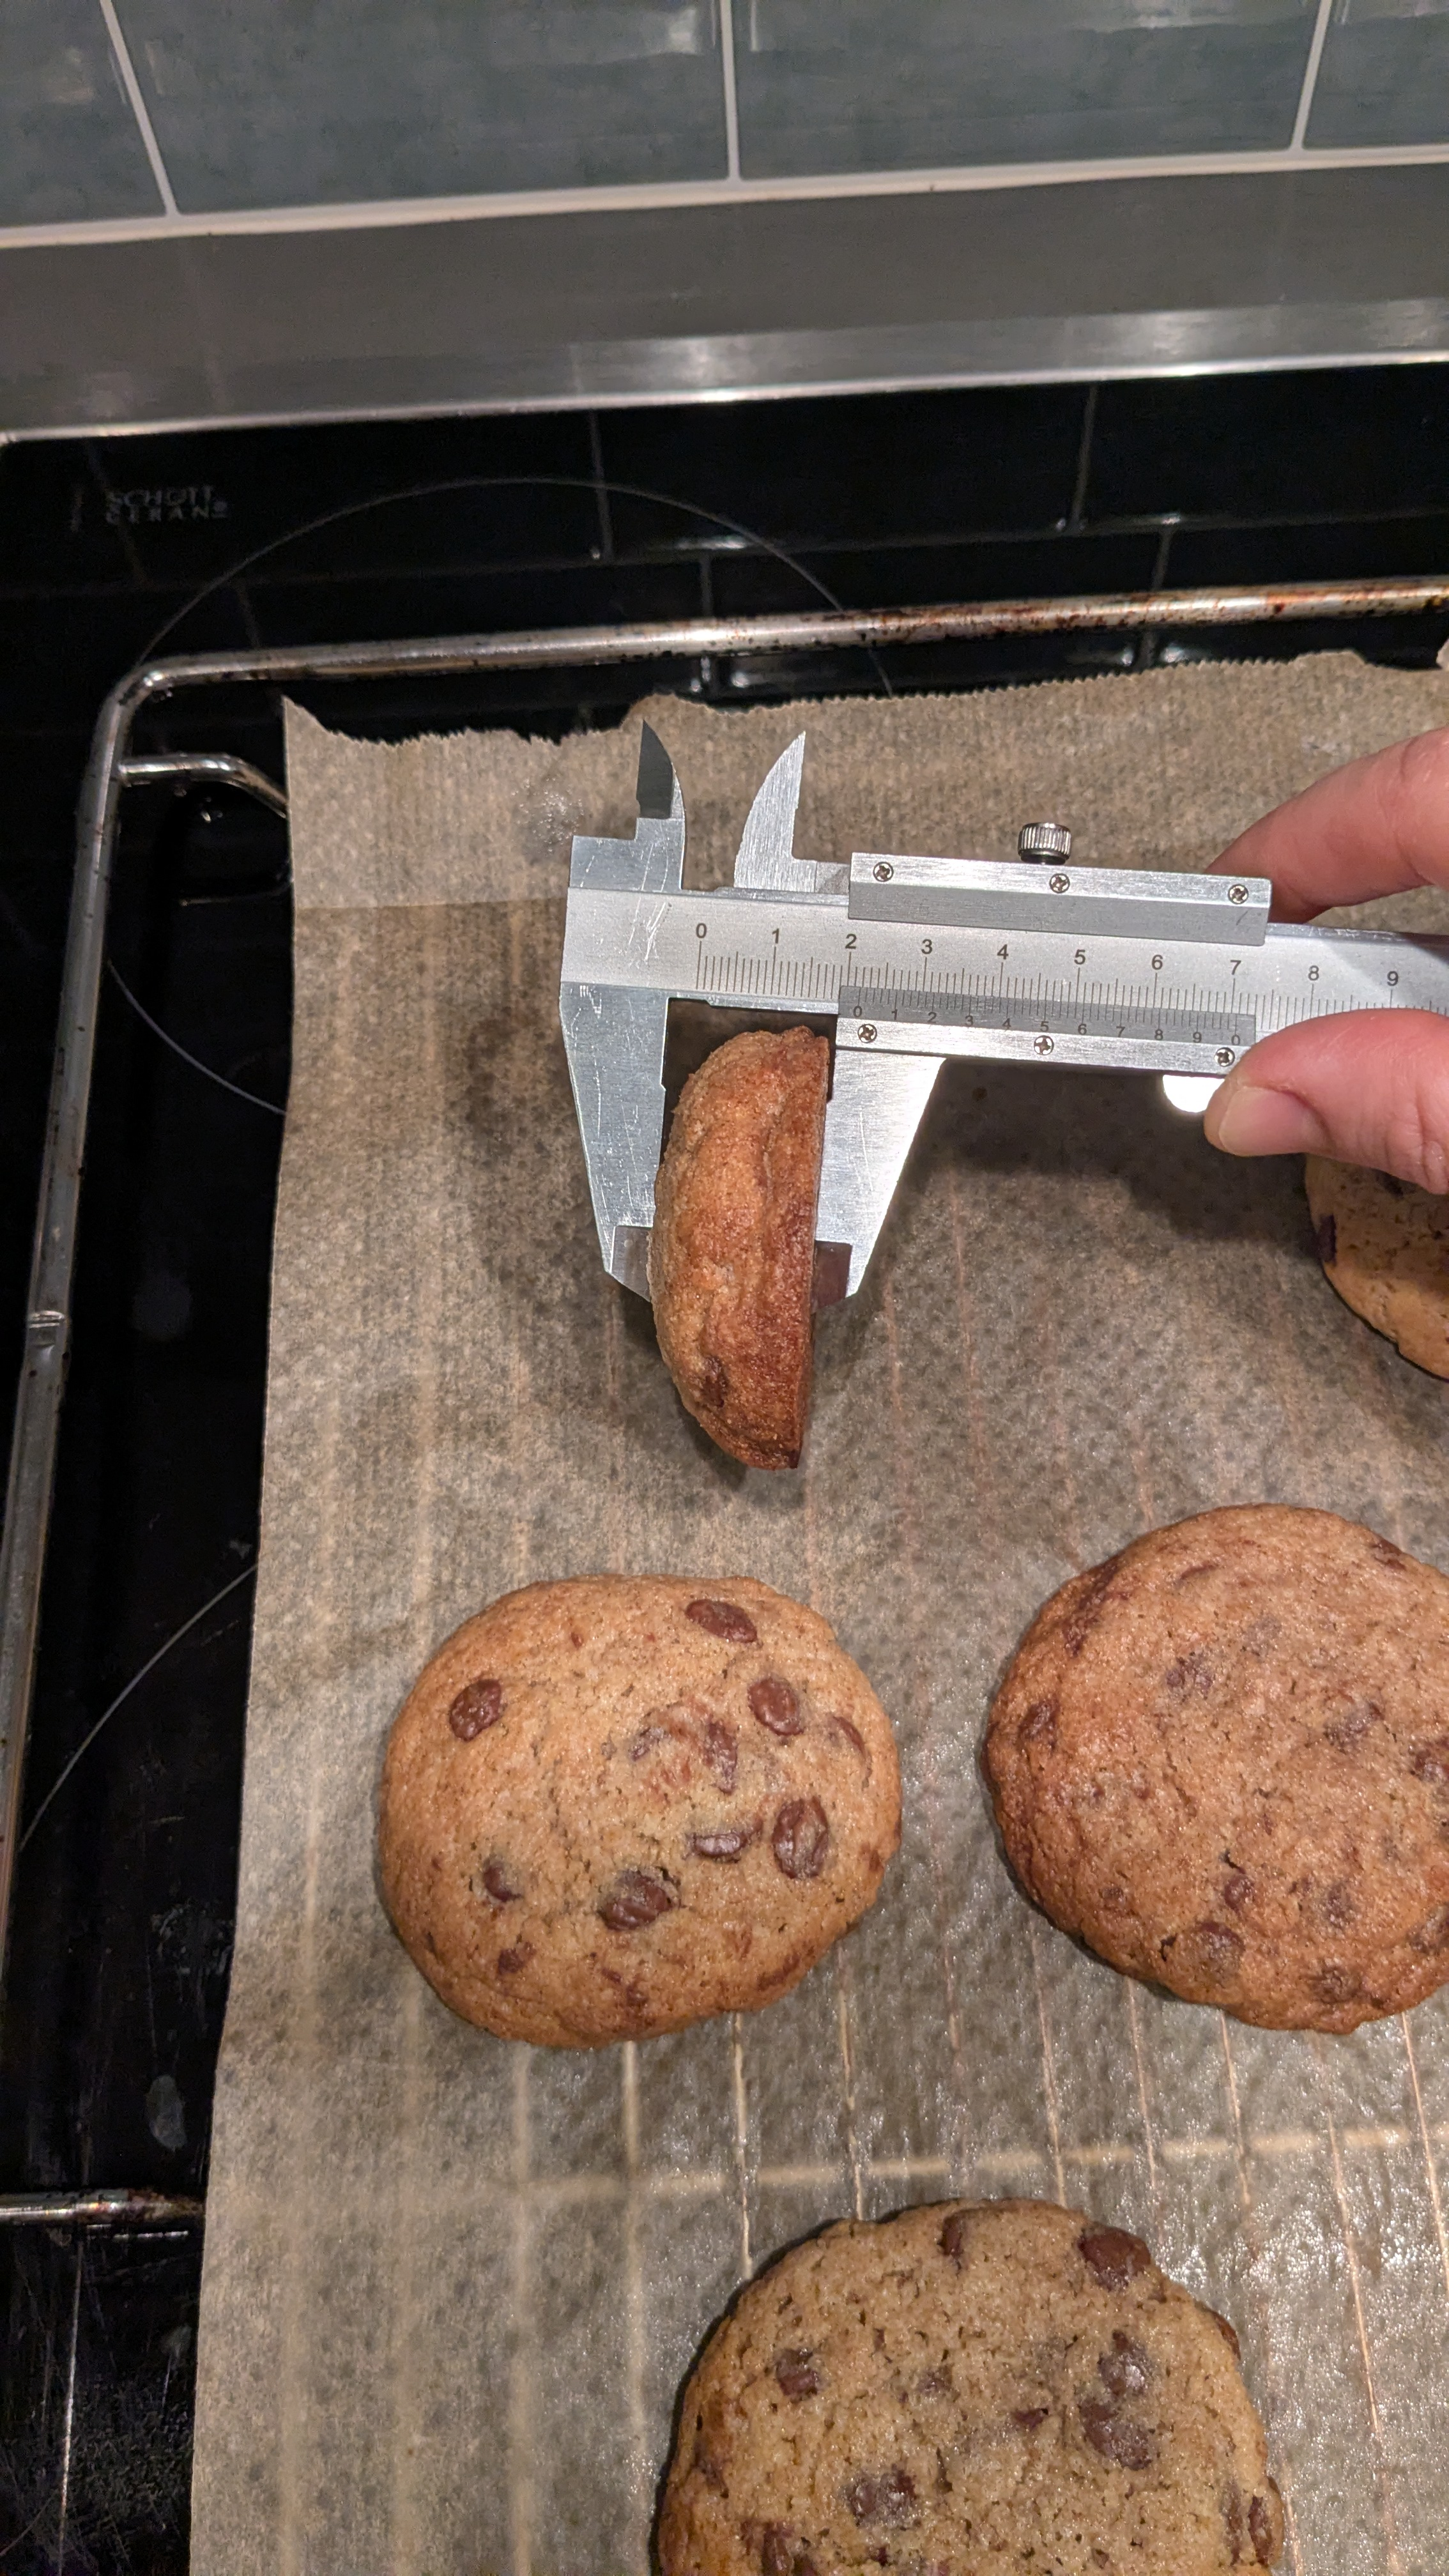
\includegraphics[width=0.5\linewidth]{figures/messung_hoehe.jpg}
    \caption{Messung der Höhe}
    \label{fig:messung_h}
\end{figure}

\chapter{Versuchsplan} \label{ch:appendix_versuch}
\vspace{-1.0\baselineskip}
\begin{table}
\centering
\caption{Versuchsplan}
\label{table:versuchsplan}
\begin{tabular}{|r|r|r|r|r|r|r|}
\hline
StdRfolge & DlaufRfolg & ZtrlPunkt & Bl"ocke & Butter\_g & Zucker\_g & Vollkornmehl\_\% \\
\hline
6  & 1  & 1 & 1 & 250 & 160 & 1  \\
1  & 2  & 1 & 1 & 120 & 160 & -1 \\
4  & 3  & 1 & 1 & 250 & 280 & -1 \\
10 & 4  & 0 & 1 & 185 & 220 & 0  \\
8  & 5  & 1 & 1 & 250 & 280 & 1  \\
7  & 6  & 1 & 1 & 120 & 280 & 1  \\
2  & 7  & 1 & 1 & 250 & 160 & -1 \\
9  & 8  & 0 & 1 & 185 & 220 & 0  \\
5  & 9  & 1 & 1 & 120 & 160 & 1  \\
3  & 10 & 1 & 1 & 120 & 280 & -1 \\
19 & 11 & 0 & 2 & 185 & 220 & 0  \\
15 & 12 & 1 & 2 & 120 & 160 & 1  \\
13 & 13 & 1 & 2 & 120 & 280 & -1 \\
20 & 14 & 0 & 2 & 185 & 220 & 0  \\
16 & 15 & 1 & 2 & 250 & 160 & 1  \\
11 & 16 & 1 & 2 & 120 & 160 & -1 \\
14 & 17 & 1 & 2 & 250 & 280 & -1 \\
18 & 18 & 1 & 2 & 250 & 280 & 1  \\
17 & 19 & 1 & 2 & 120 & 280 & 1  \\
12 & 20 & 1 & 2 & 250 & 160 & -1 \\
28 & 21 & 1 & 3 & 250 & 280 & 1  \\
27 & 22 & 1 & 3 & 120 & 280 & 1  \\
22 & 23 & 1 & 3 & 250 & 160 & -1 \\
30 & 24 & 0 & 3 & 185 & 220 & 0  \\
29 & 25 & 0 & 3 & 185 & 220 & 0  \\
25 & 26 & 1 & 3 & 120 & 160 & 1  \\
23 & 27 & 1 & 3 & 120 & 280 & -1 \\
26 & 28 & 1 & 3 & 250 & 160 & 1  \\
21 & 29 & 1 & 3 & 120 & 160 & -1 \\
24 & 30 & 1 & 3 & 250 & 280 & -1 \\
\hline
\end{tabular}
\end{table}


\chapter{Ergebnisse} \label{ch:appendix_ergebnisse}
\vspace{-1.0\baselineskip}
\begin{table}[H]
\centering
\caption{Versuchsergebnisse: Durchmesser und Höhe in mm}
\label{tab:ergebnisse}
\begin{tabular}{|r|r|r|r|r|}
\hline
DlaufRfolg & Durchmesser\_1 & Durchmesser\_2 & Höhe & Durchsch\_Durchmesser \\
\hline
1 & 59 & 61 & 23 & 60 \\
2 & 61 & 64 & 21 & 62,5 \\
3 & 89 & 83 & 8 & 86 \\
4 & 66 & 73 & 16 & 69,5 \\
5 & 76 & 76 & 14 & 76 \\
6 & 67 & 67 & 16 & 67 \\
7 & 73 & 69 & 19 & 71 \\
8 & 70 & 72 & 15 & 71 \\
9 & 59 & 56 & 22 & 57,5 \\
10 & 79 & 78 & 13 & 78,5 \\
\hline
11 & 69 & 69 & 16 & 69 \\
12 & 58 & 57 & 22 & 57,5 \\
13 & 80 & 76 & 11 & 78 \\
14 & 69 & 70 & 16 & 69,5 \\
15 & 64 & 64 & 18 & 64 \\
16 & 66 & 64 & 20 & 65 \\
17 & 90 & 88 & 9 & 89 \\
18 & 77 & 83 & 13 & 80 \\
19 & 69 & 69 & 17 & 69 \\
20 & 75 & 75 & 17 & 75 \\
\hline
21 & 77 & 78 & 15 & 77,5 \\
22 & 70 & 70 & 16 & 70 \\
23 & 75 & 73 & 17 & 74 \\
24 & 73 & 70 & 17 & 71,5 \\
25 & 74 & 69 & 15 & 71,5 \\
26 & 61 & 59 & 22 & 60 \\
27 & 80 & 80 & 13 & 80 \\
28 & 67 & 67 & 21 & 67 \\
29 & 65 & 68 & 19 & 66,5 \\
30 & 94 & 89 & 9 & 91,5 \\
\hline
\end{tabular}
\end{table}


\chapter{Dokumentation der Durchführung} \label{ch:appendix_durchf}
\vspace{-1.0\baselineskip}

\begin{figure}[H]
\centering
\begin{subfigure}{0.49\textwidth}
    \centering
    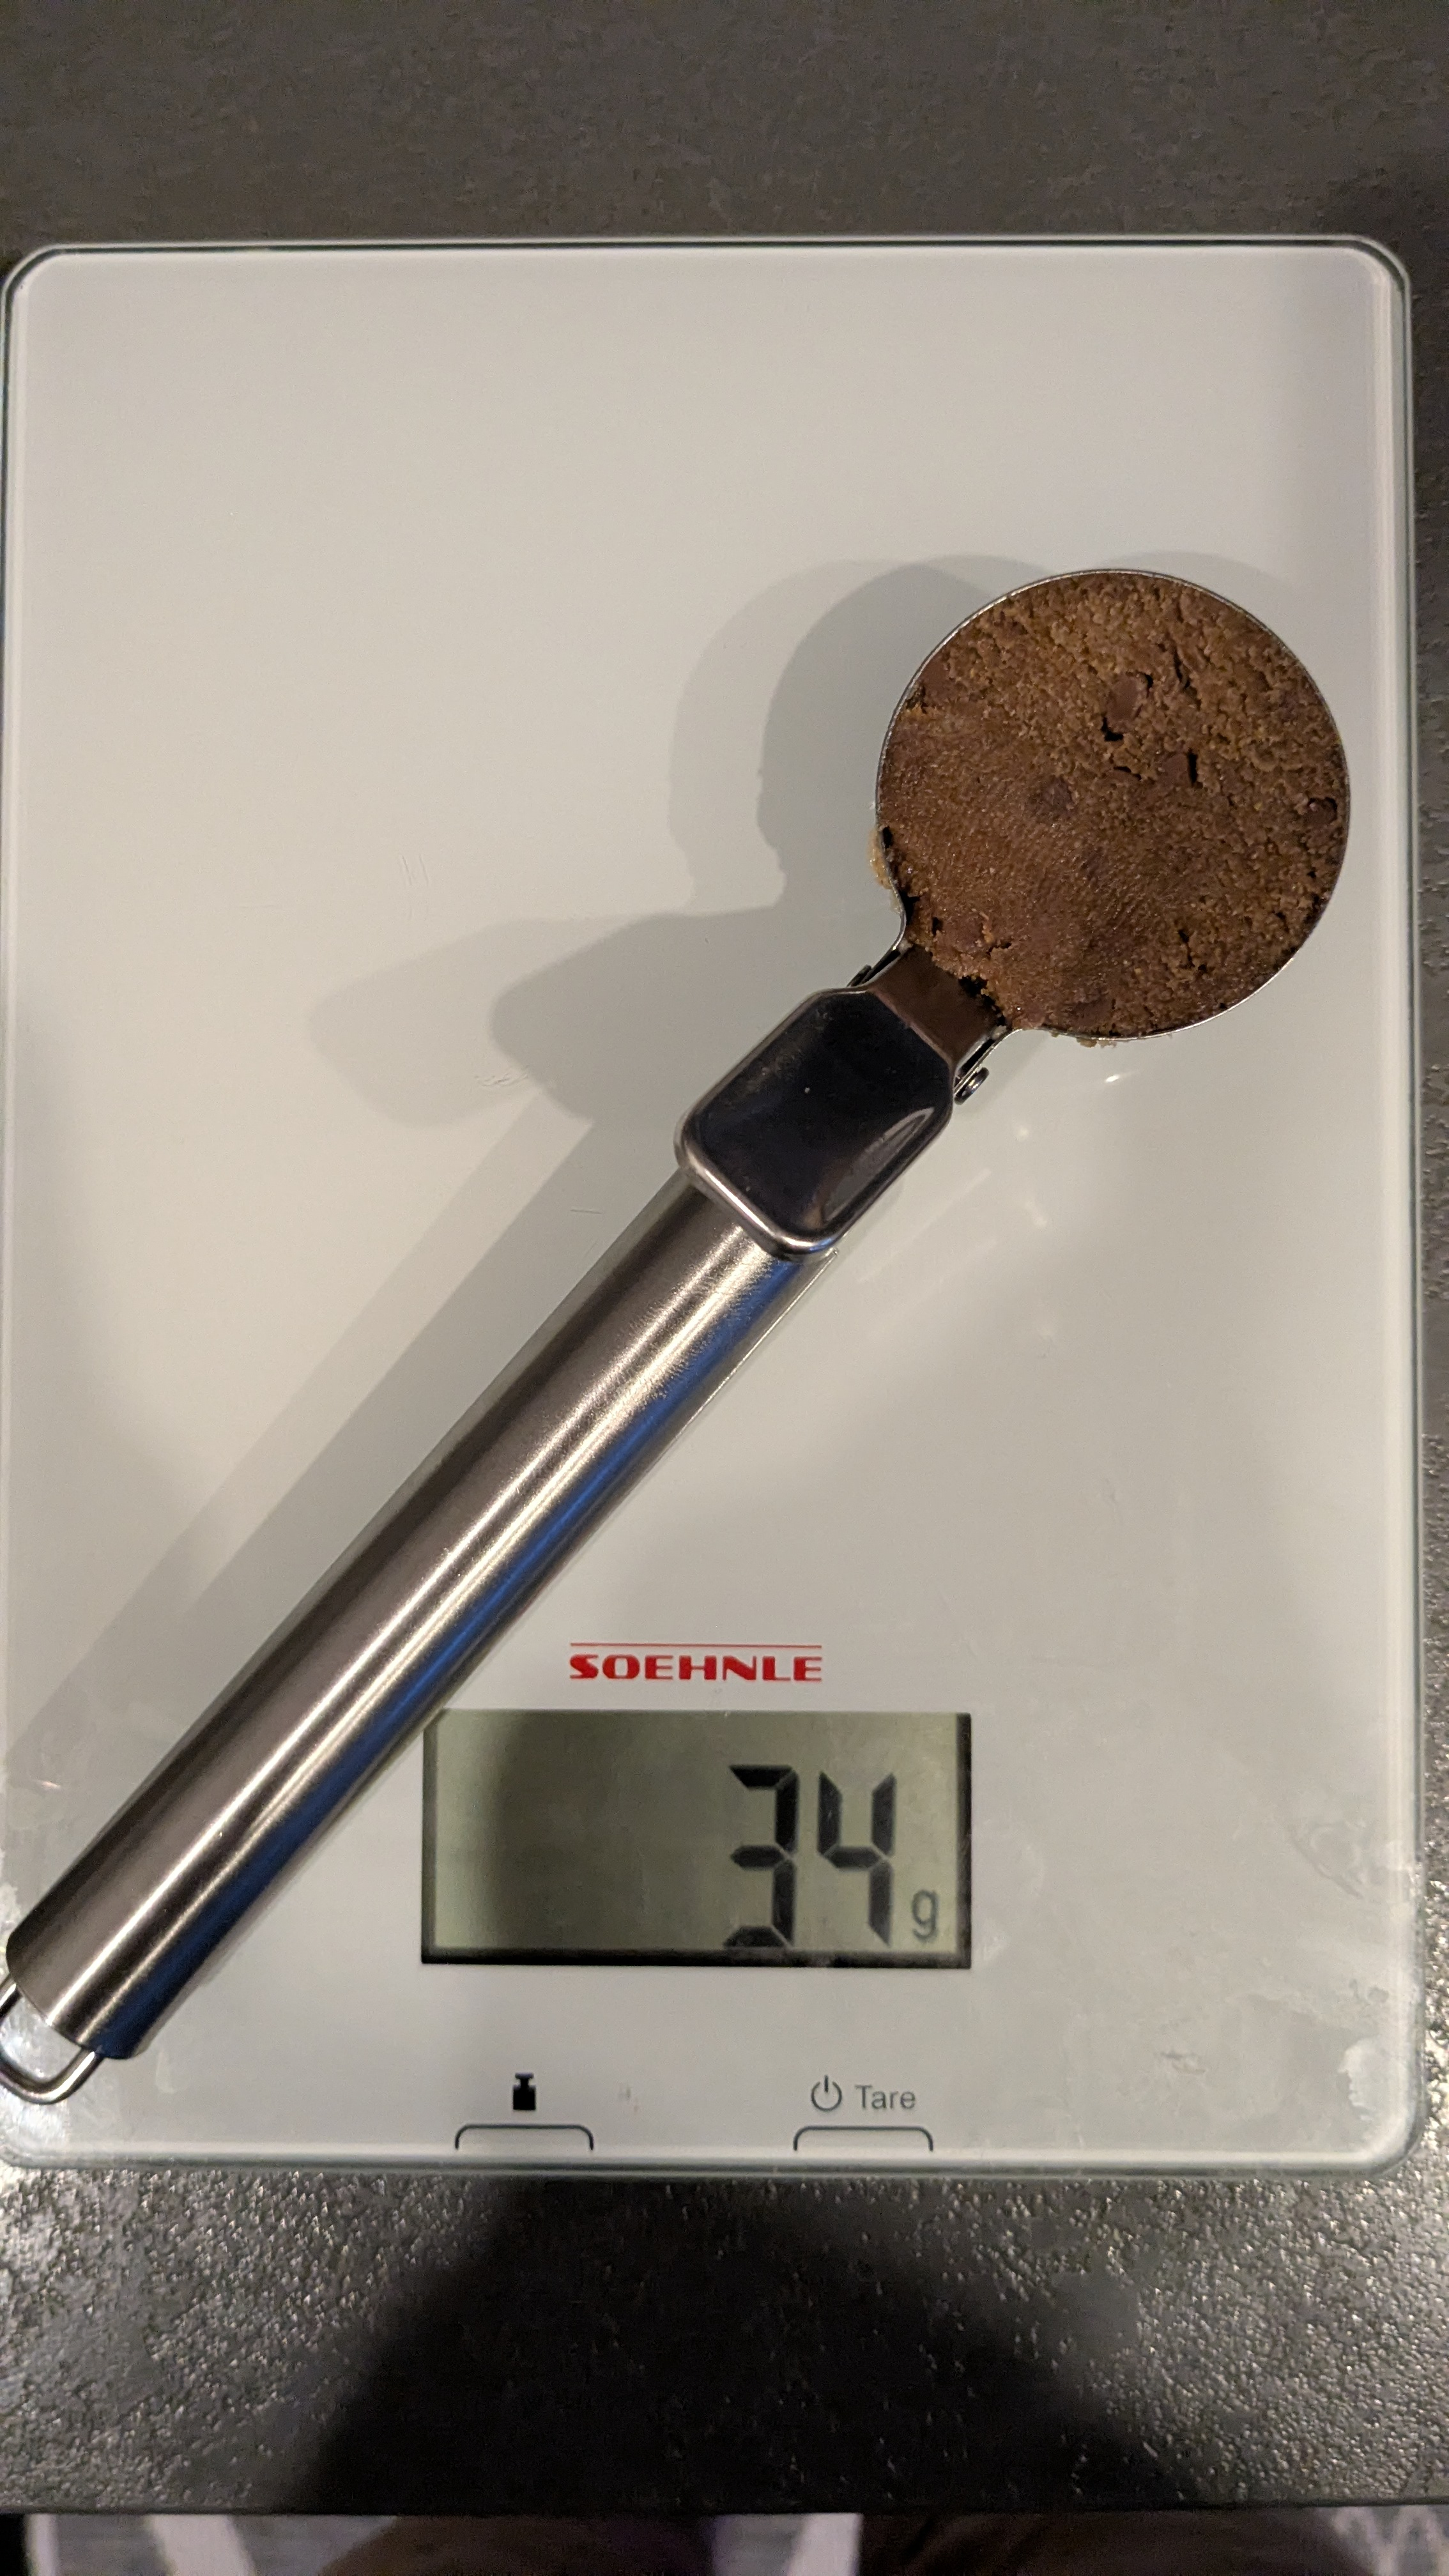
\includegraphics[width=\textwidth]{figures/portionierung_gewicht.jpg}
    \caption{Portionierung eines Cookies mit Gewichtsmessung}
    \label{fig:portionierung}
\end{subfigure}\hfill
\begin{subfigure}{0.49\textwidth}
    \centering
    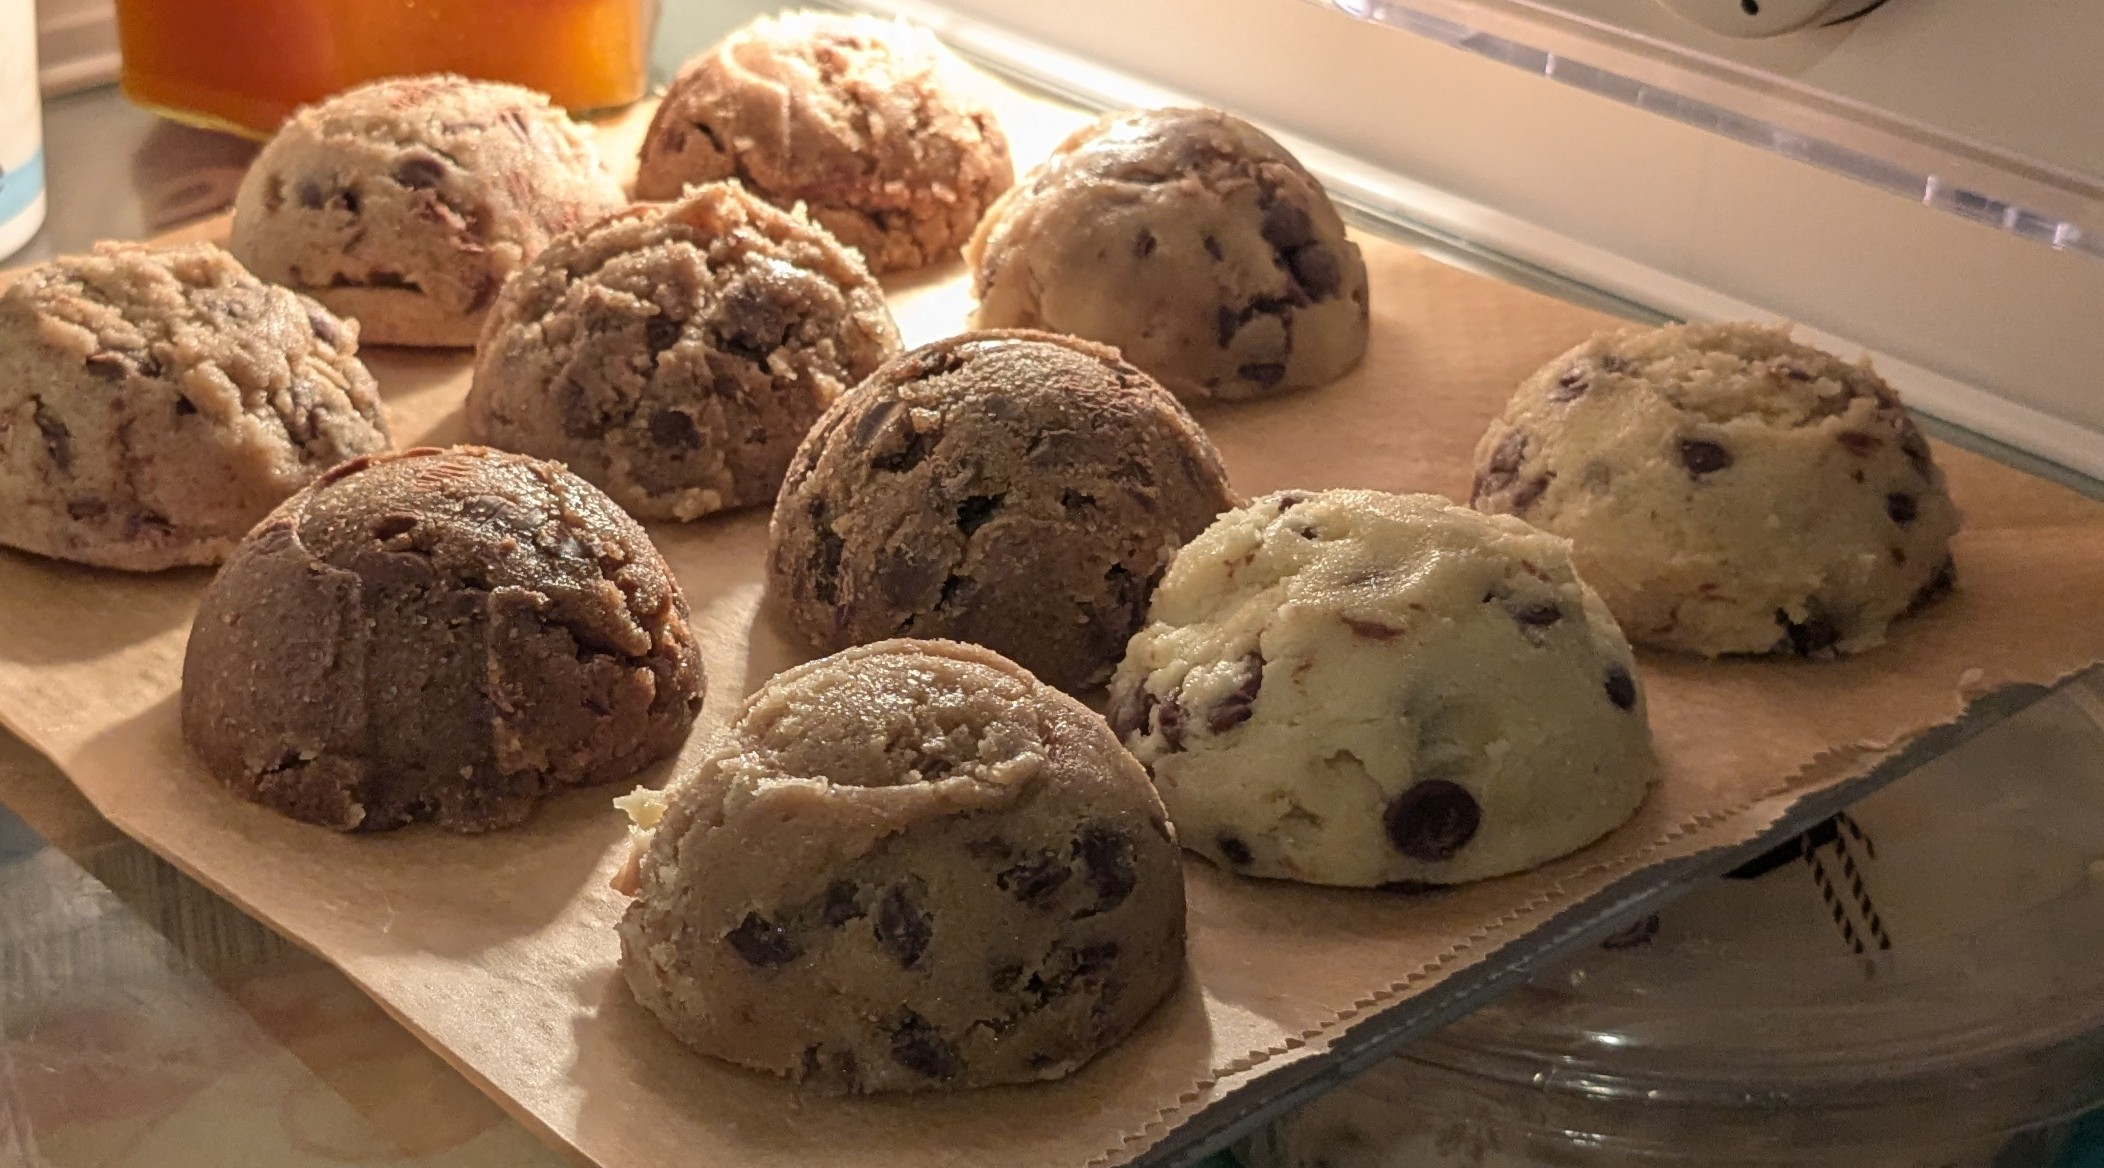
\includegraphics[width=\textwidth]{figures/portionen_vorbereitung_klein.jpg}
    \caption{Kühlung der Cookies während des Portionierens}
    \label{fig:kühlung}
\end{subfigure}
\caption{Portionierung und Vorbereitung}
\label{fig:portionierung}
\end{figure}

\begin{figure}[H]
\centering
\begin{subfigure}{0.49\textwidth}
    \centering
    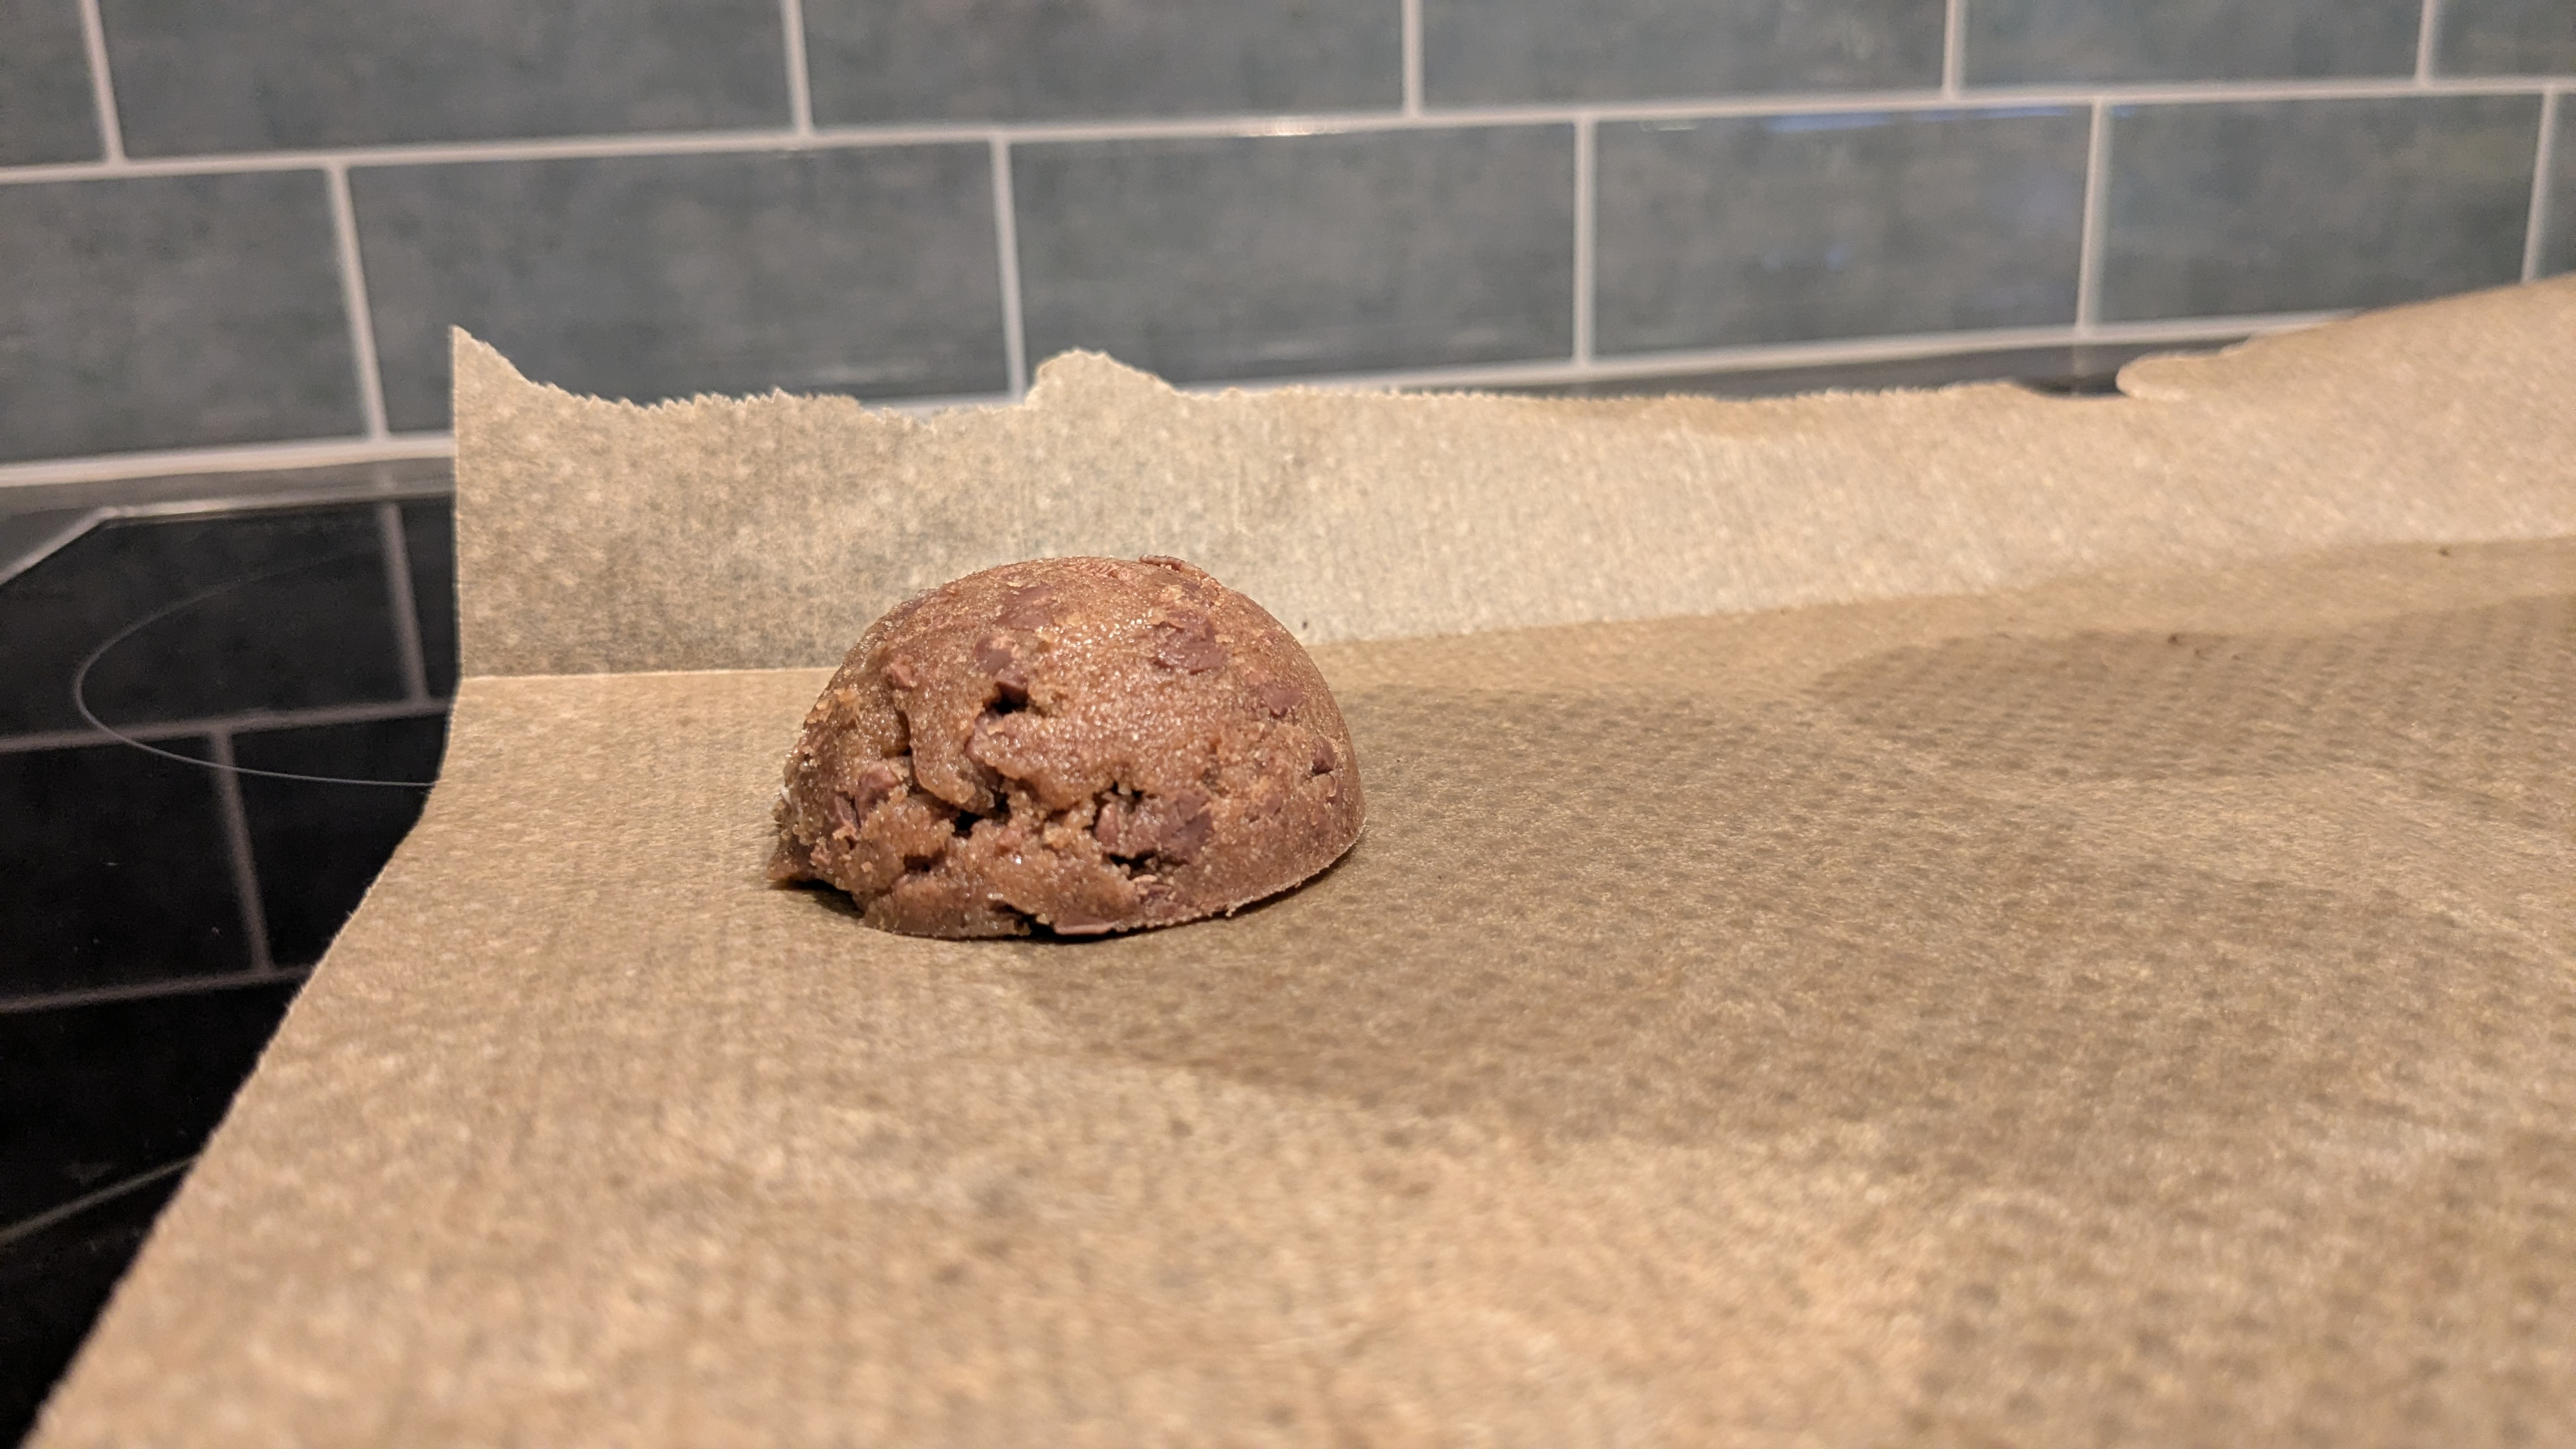
\includegraphics[width=\textwidth]{figures/portion_seitlich.jpg}
    \caption{Seitliche Sicht}
    \label{fig:portion_seitlich}
\end{subfigure}\hfill
\begin{subfigure}{0.49\textwidth}
    \centering
    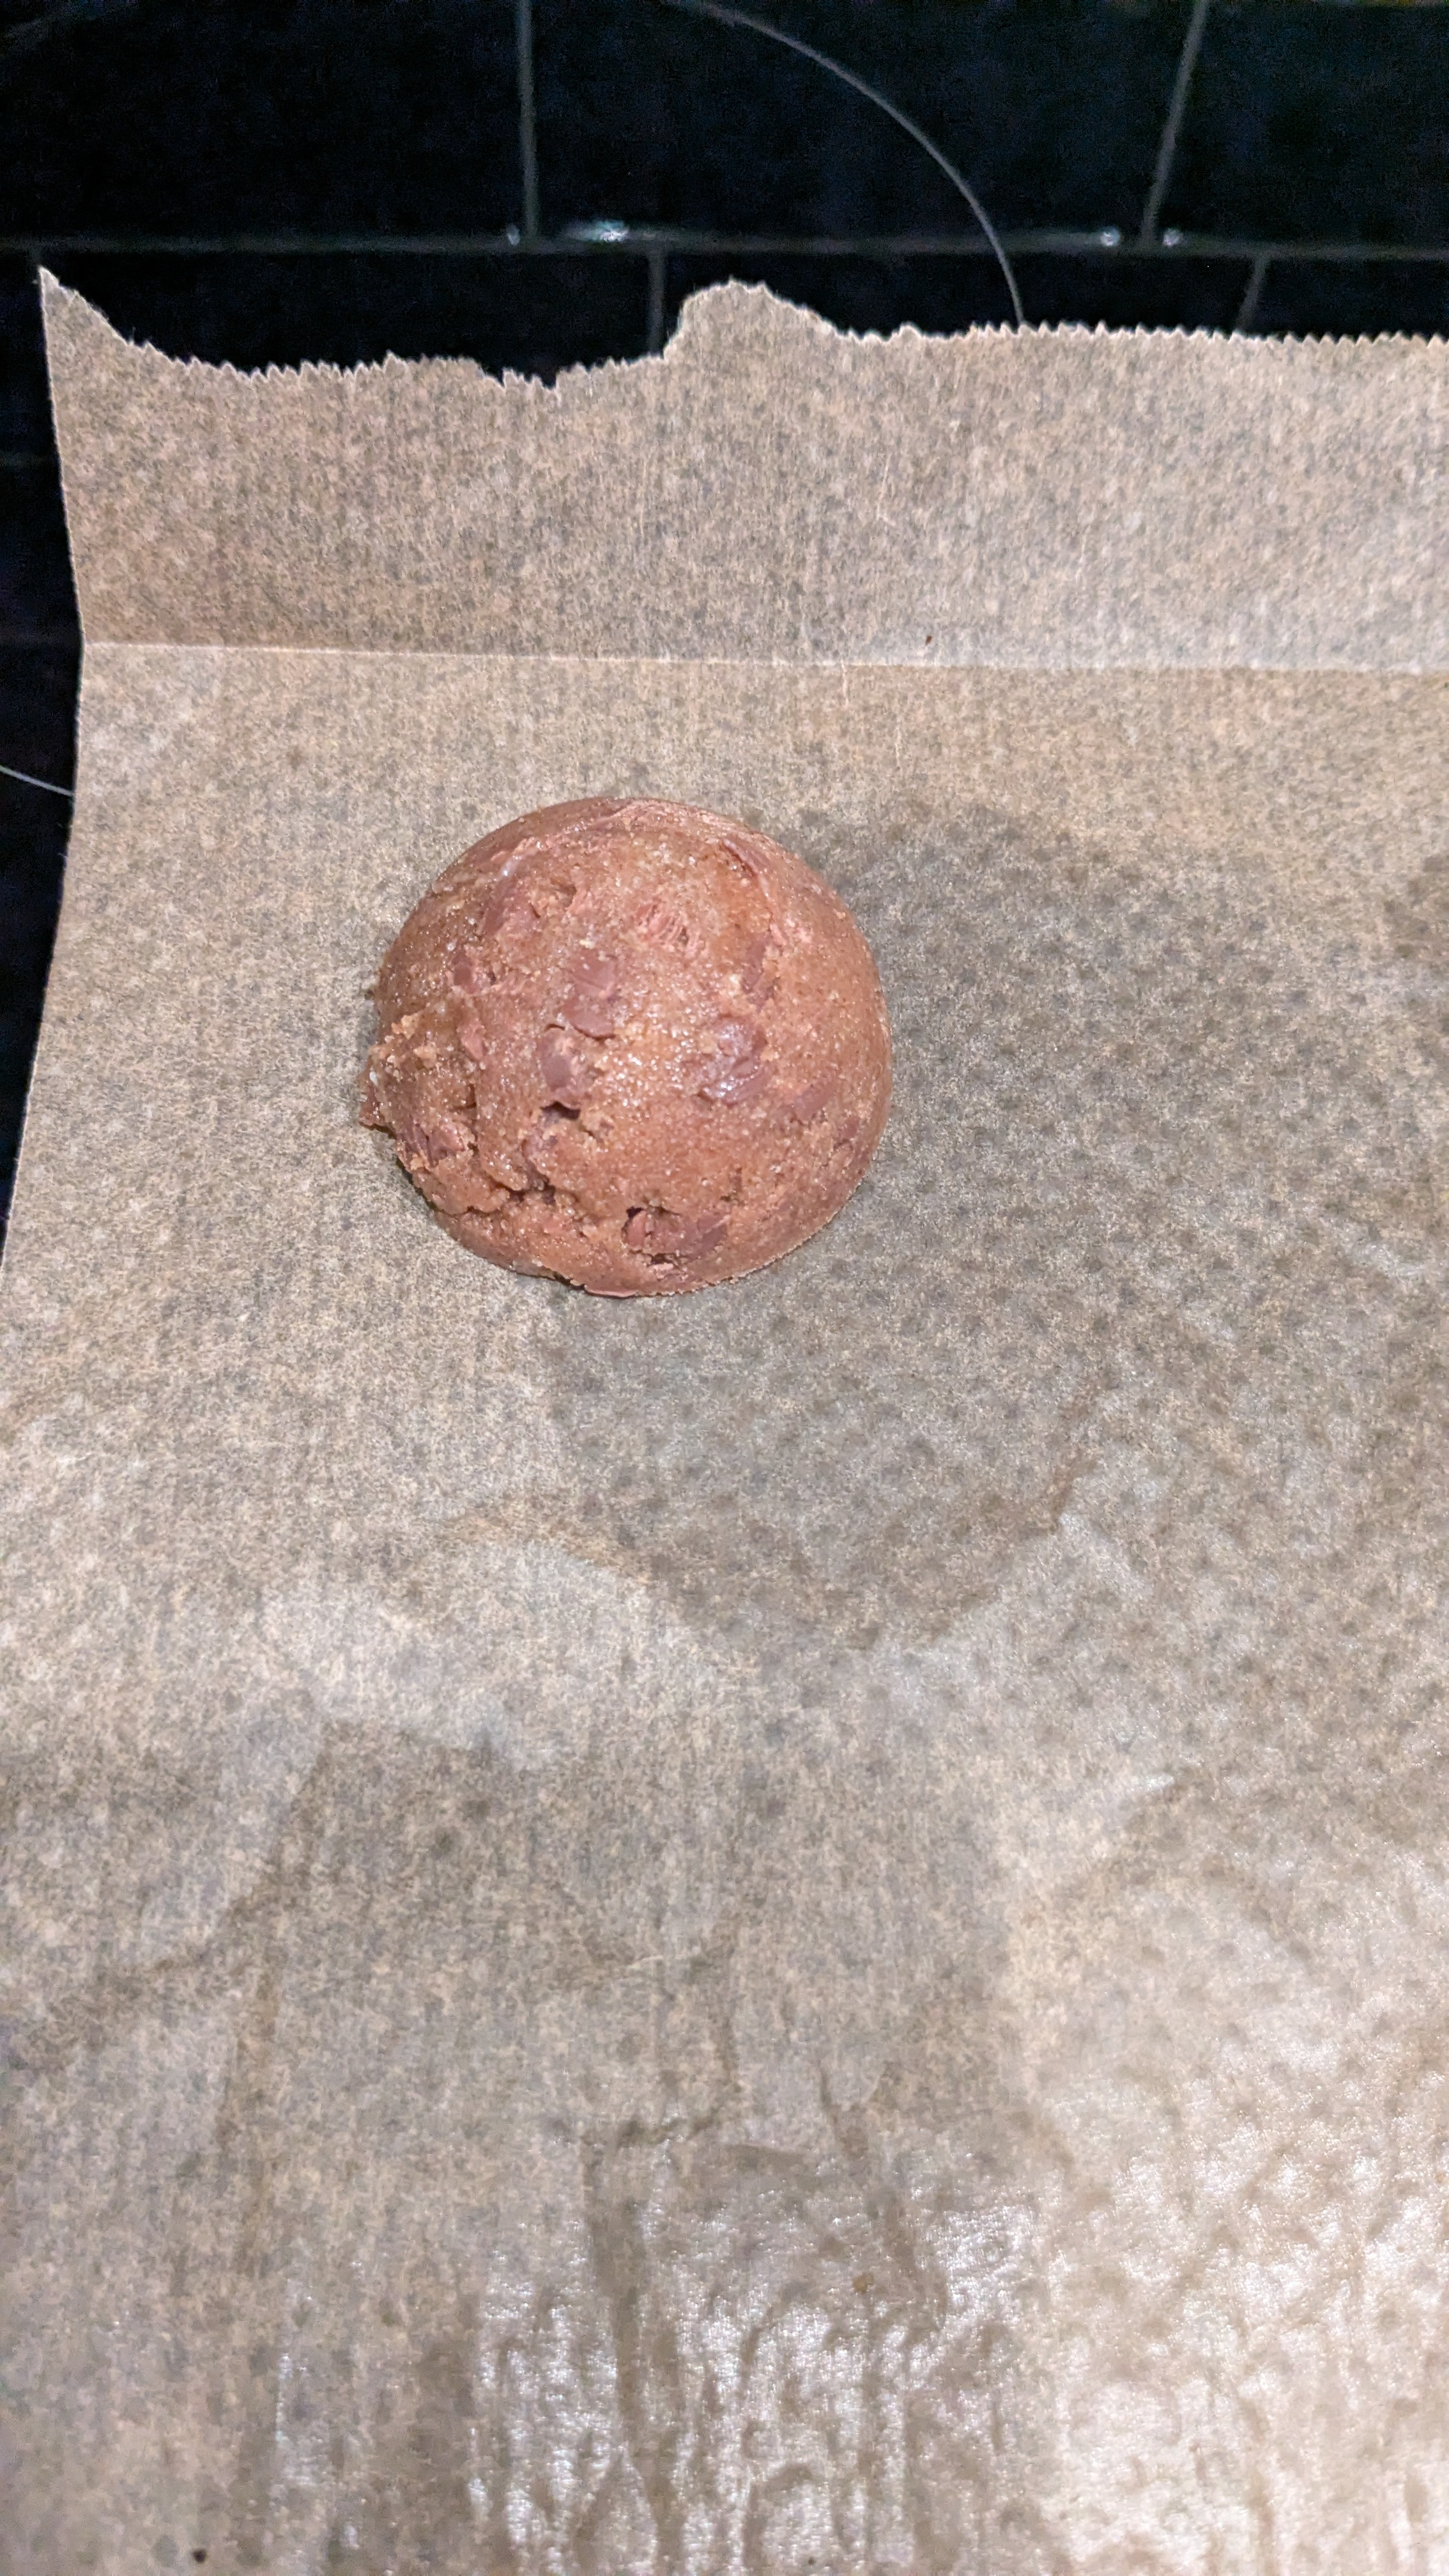
\includegraphics[width=\textwidth]{figures/portion_oben.jpg}
    \caption{Draufsicht}
    \label{fig:portion_draufsicht}
\end{subfigure}
\caption{Ansicht einer Portion}
\label{fig:portion}
\end{figure}

\begin{figure}[H]
\centering
\begin{subfigure}{0.49\textwidth}
\centering
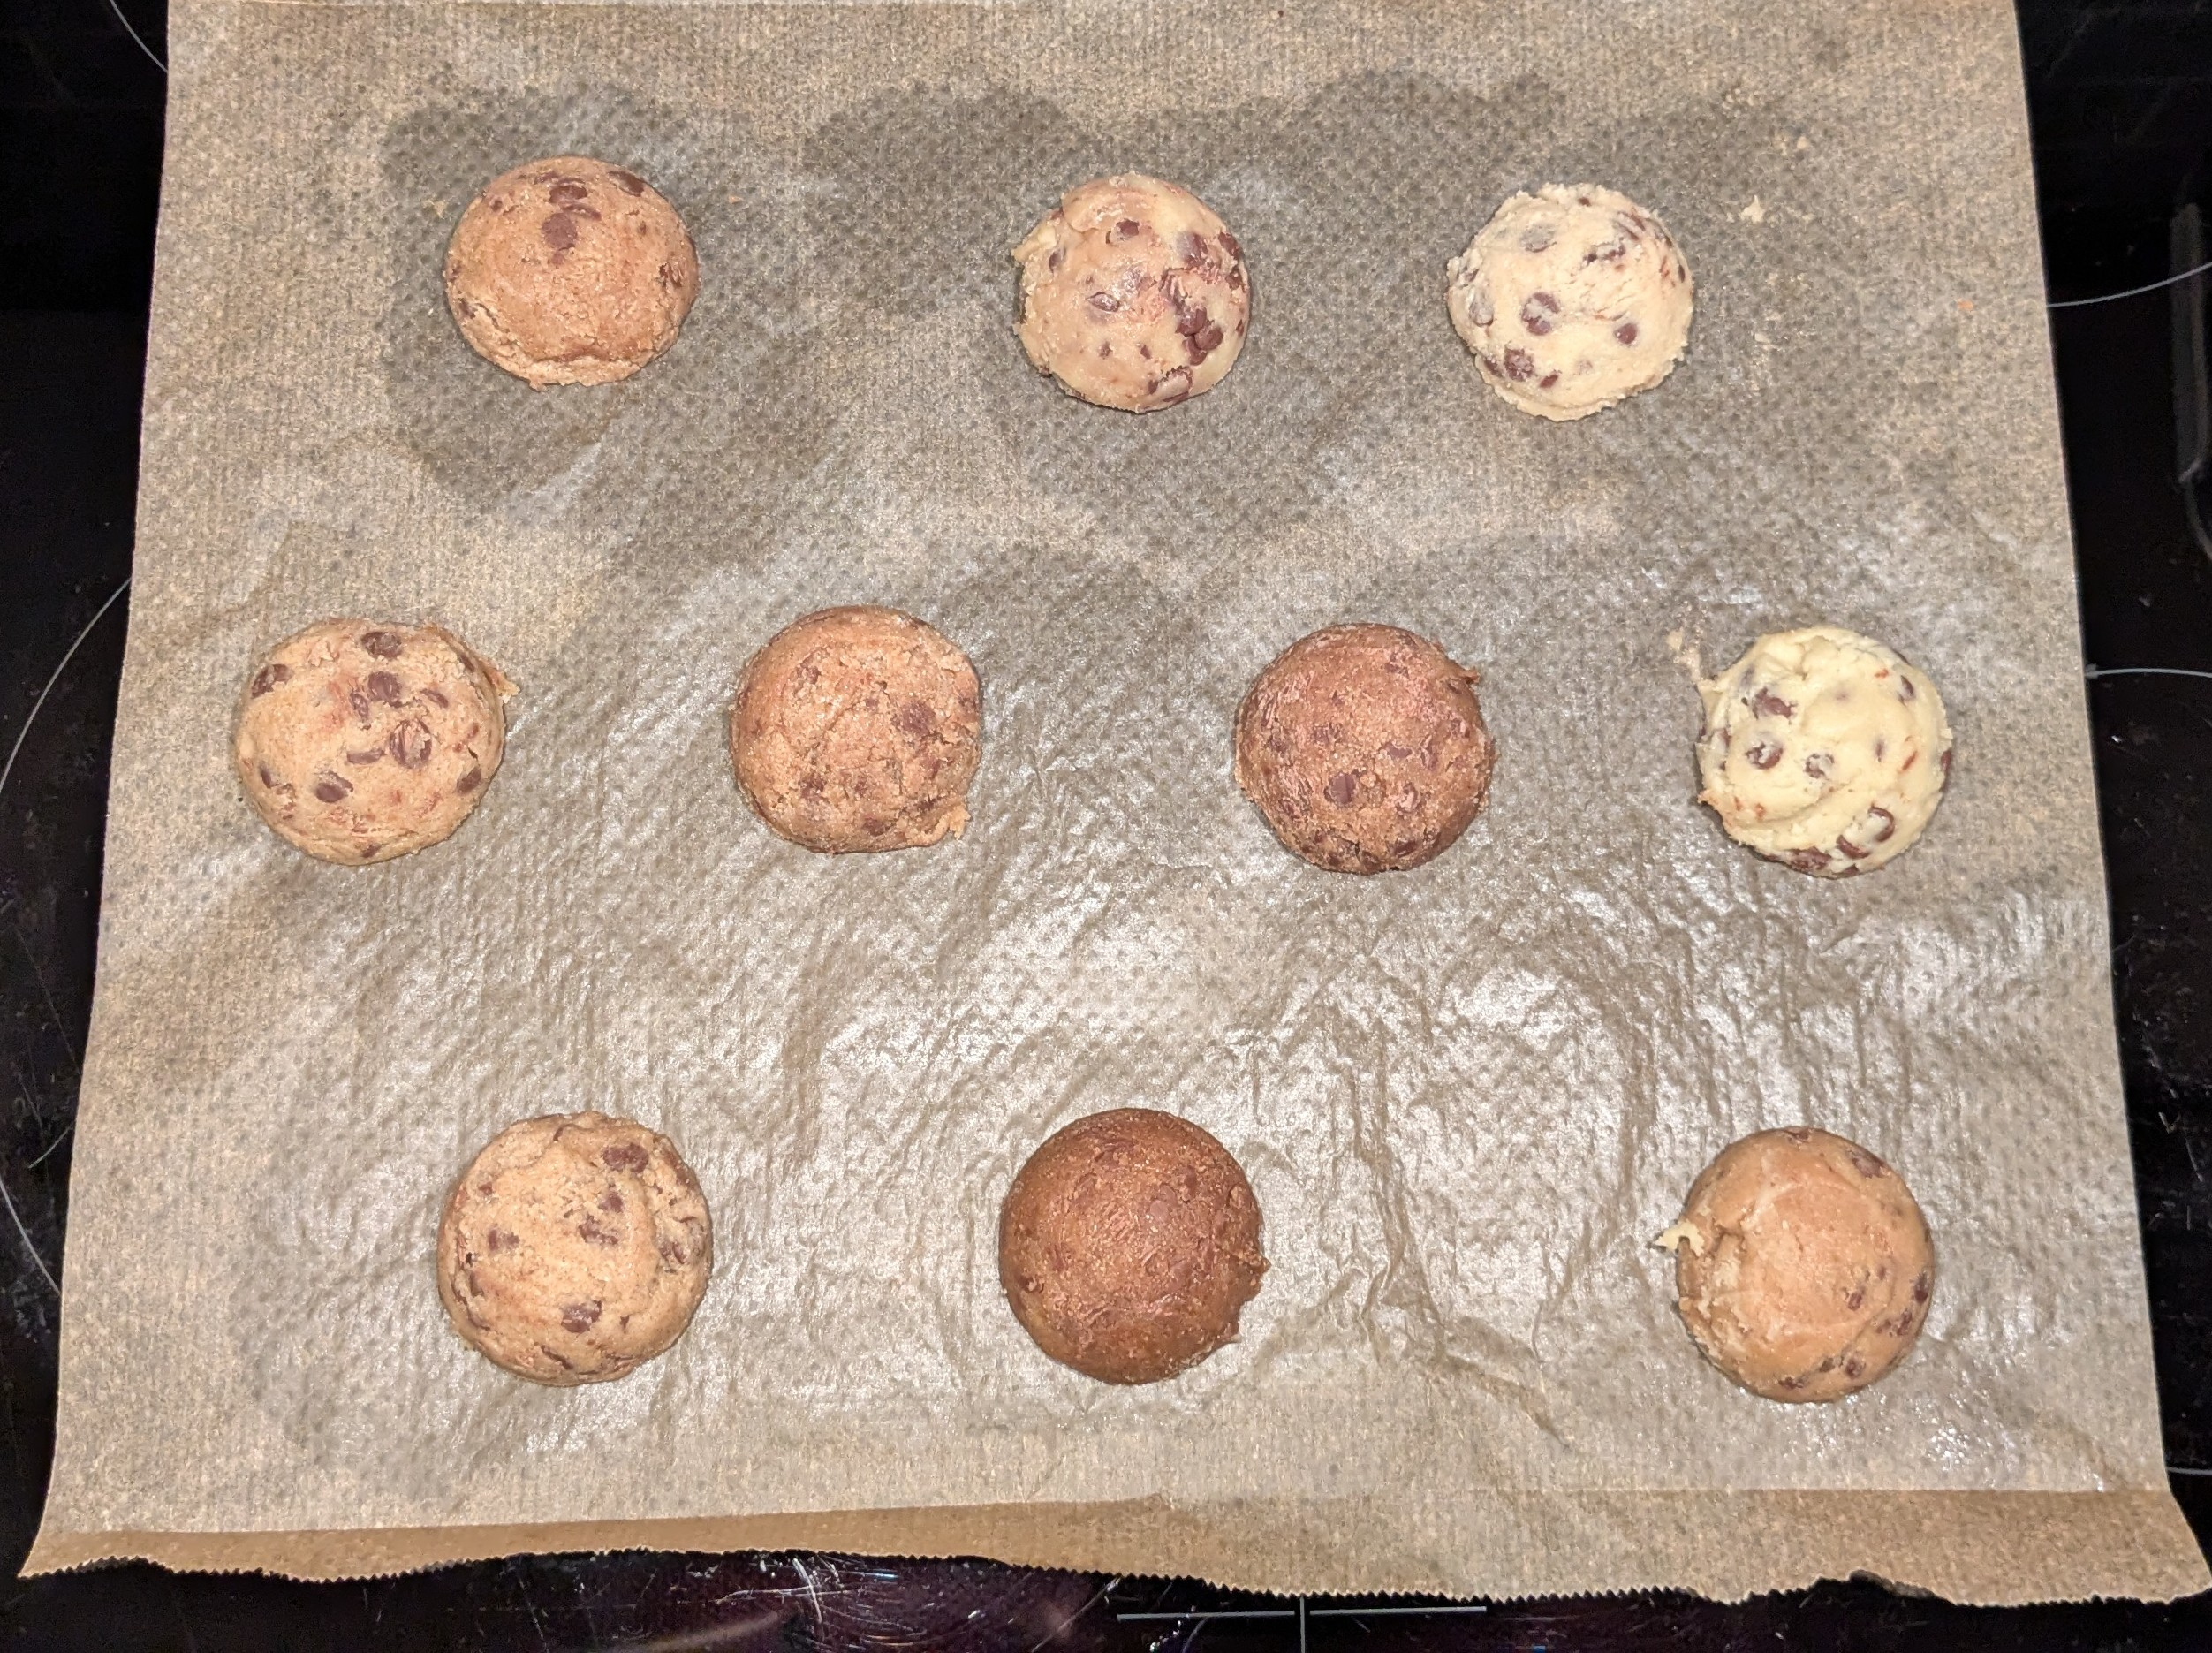
\includegraphics[width = \textwidth]{figures/block1_1_vorher.jpg}
\caption{Teigrohlinge vor dem Backen}
\label{fig:block1_1_vorher}
\end{subfigure}\hfill
\begin{subfigure}{0.49\textwidth}
\centering
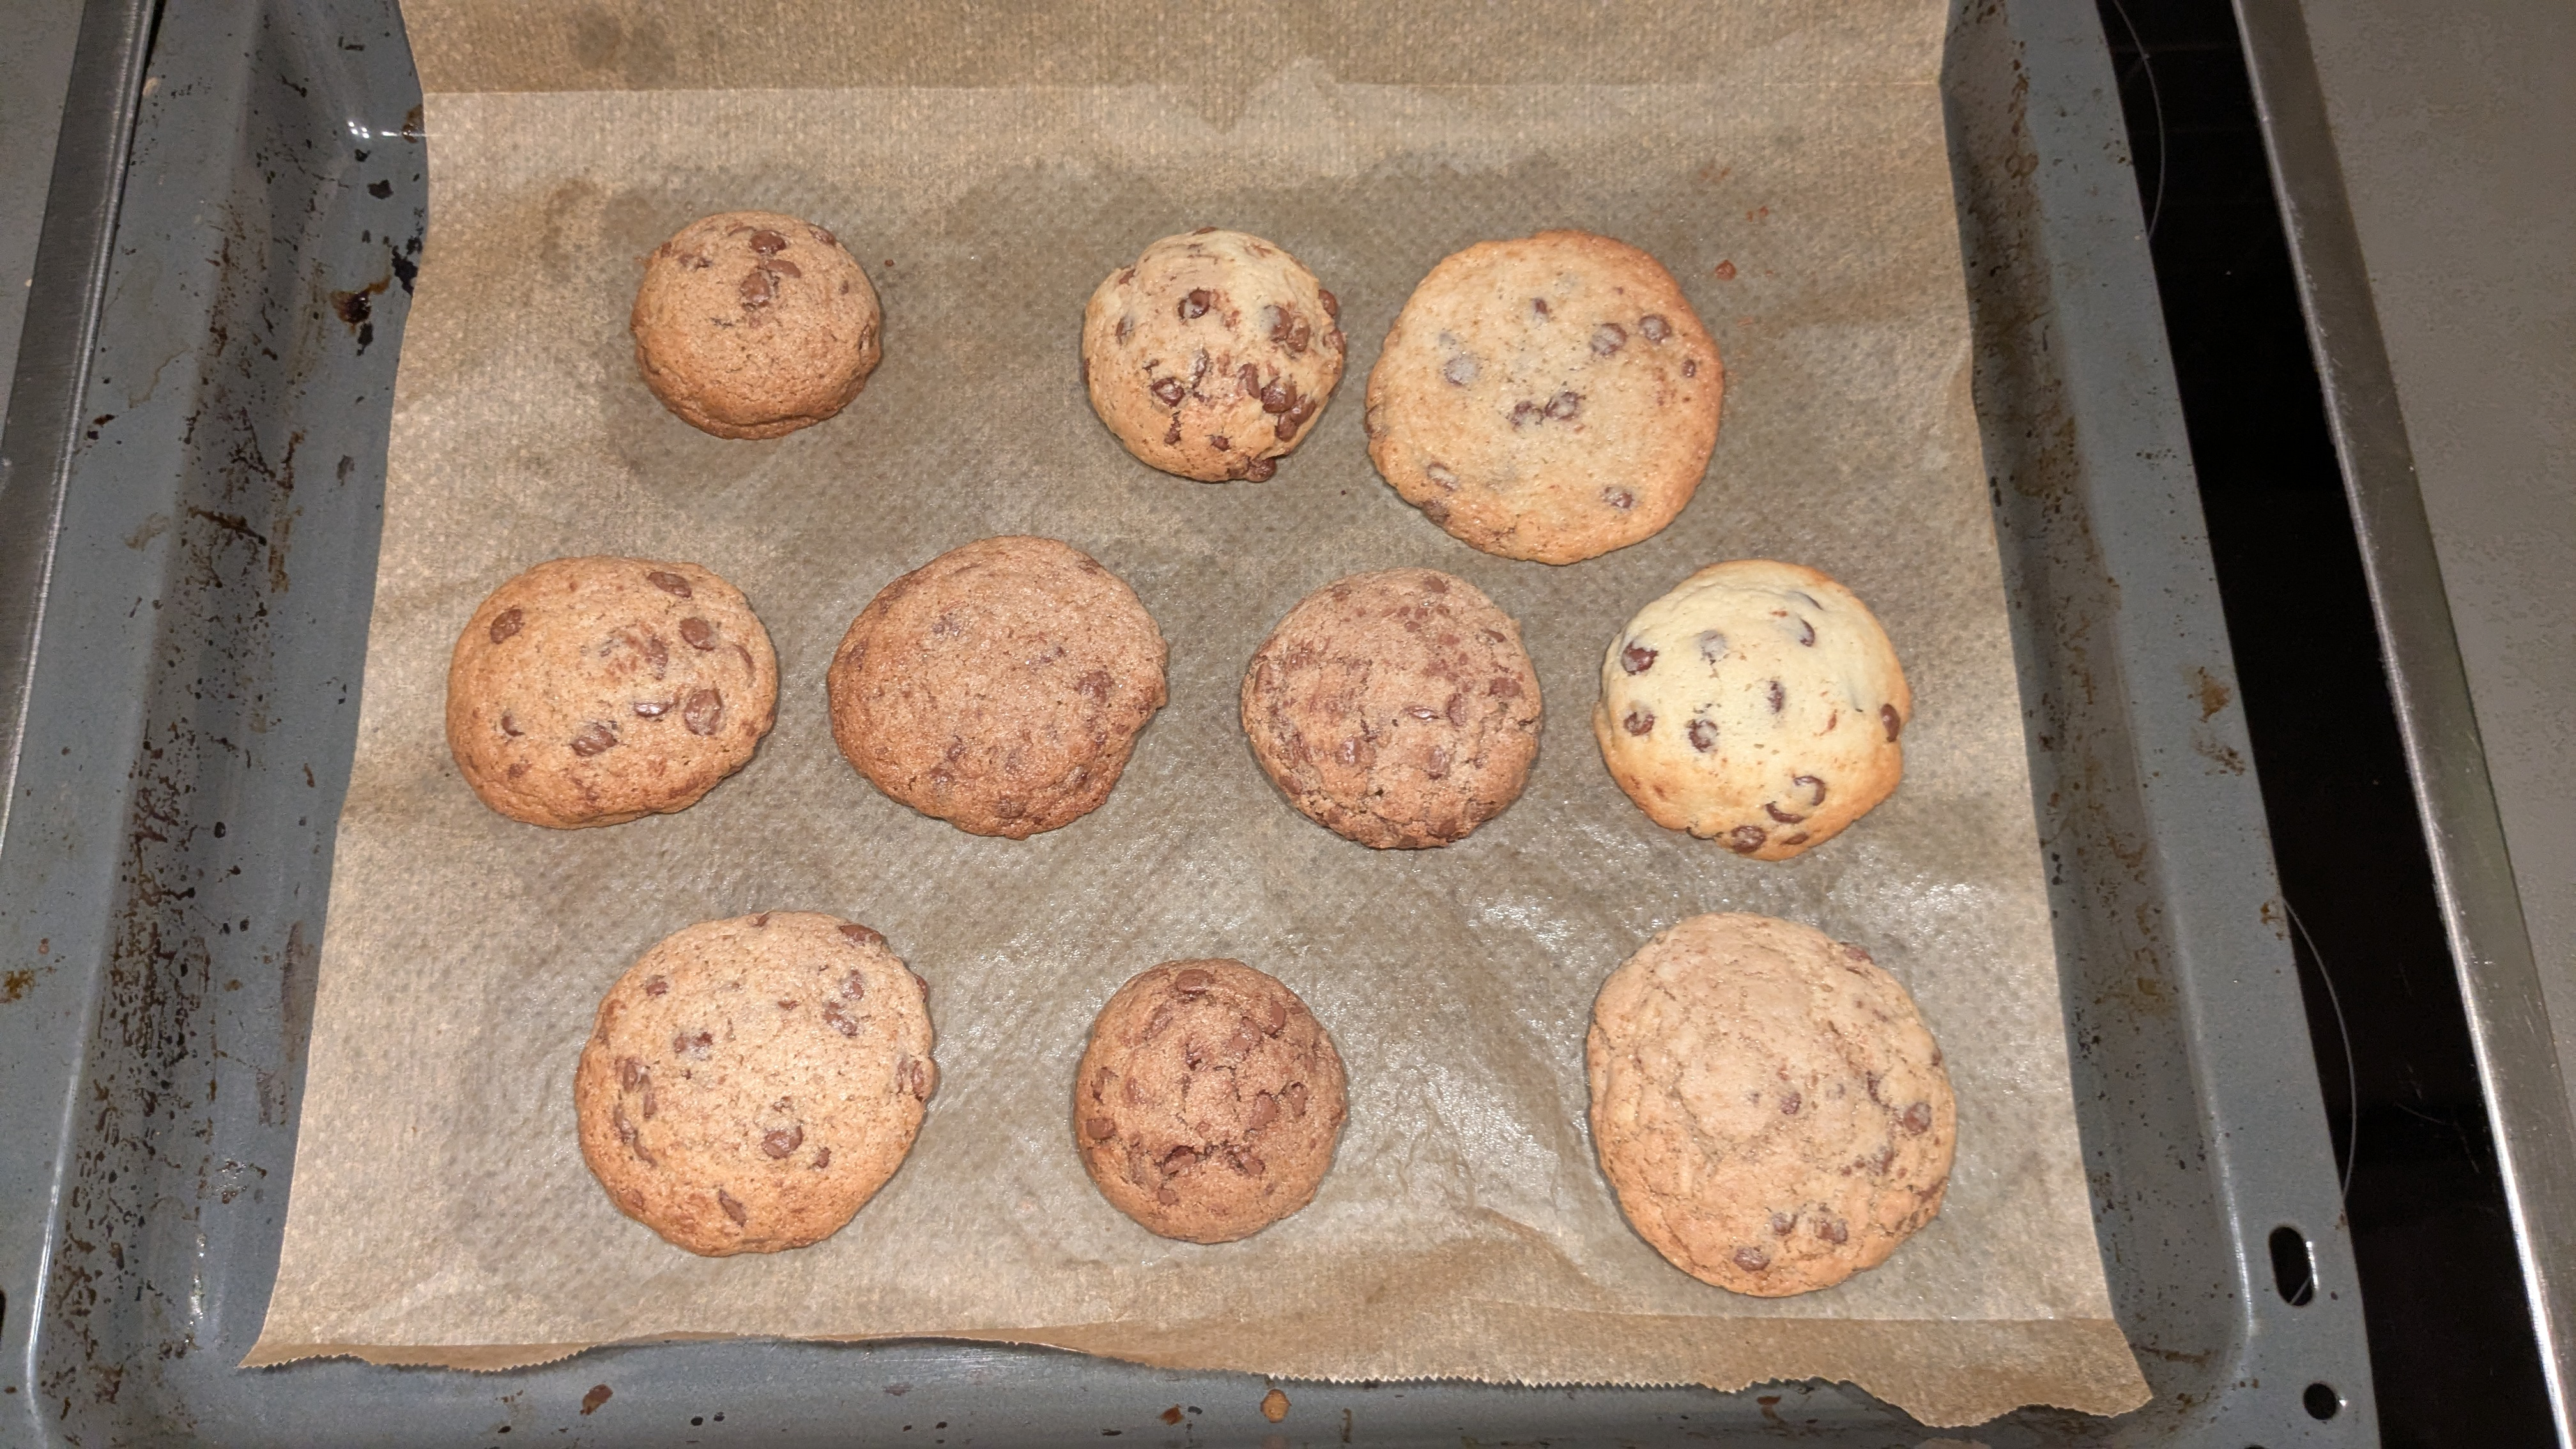
\includegraphics[width = \textwidth]{figures/block1_4_nacher.jpg}
\caption{Cookies nach dem Backvorgang}
\label{fig:block1_4_nacher}
\end{subfigure}
\caption{Backvorgang der ersten Replikation}
\label{fig:block_1}
\end{figure}

\begin{figure}[H]
\centering
\begin{subfigure}{0.49\textwidth}
\centering
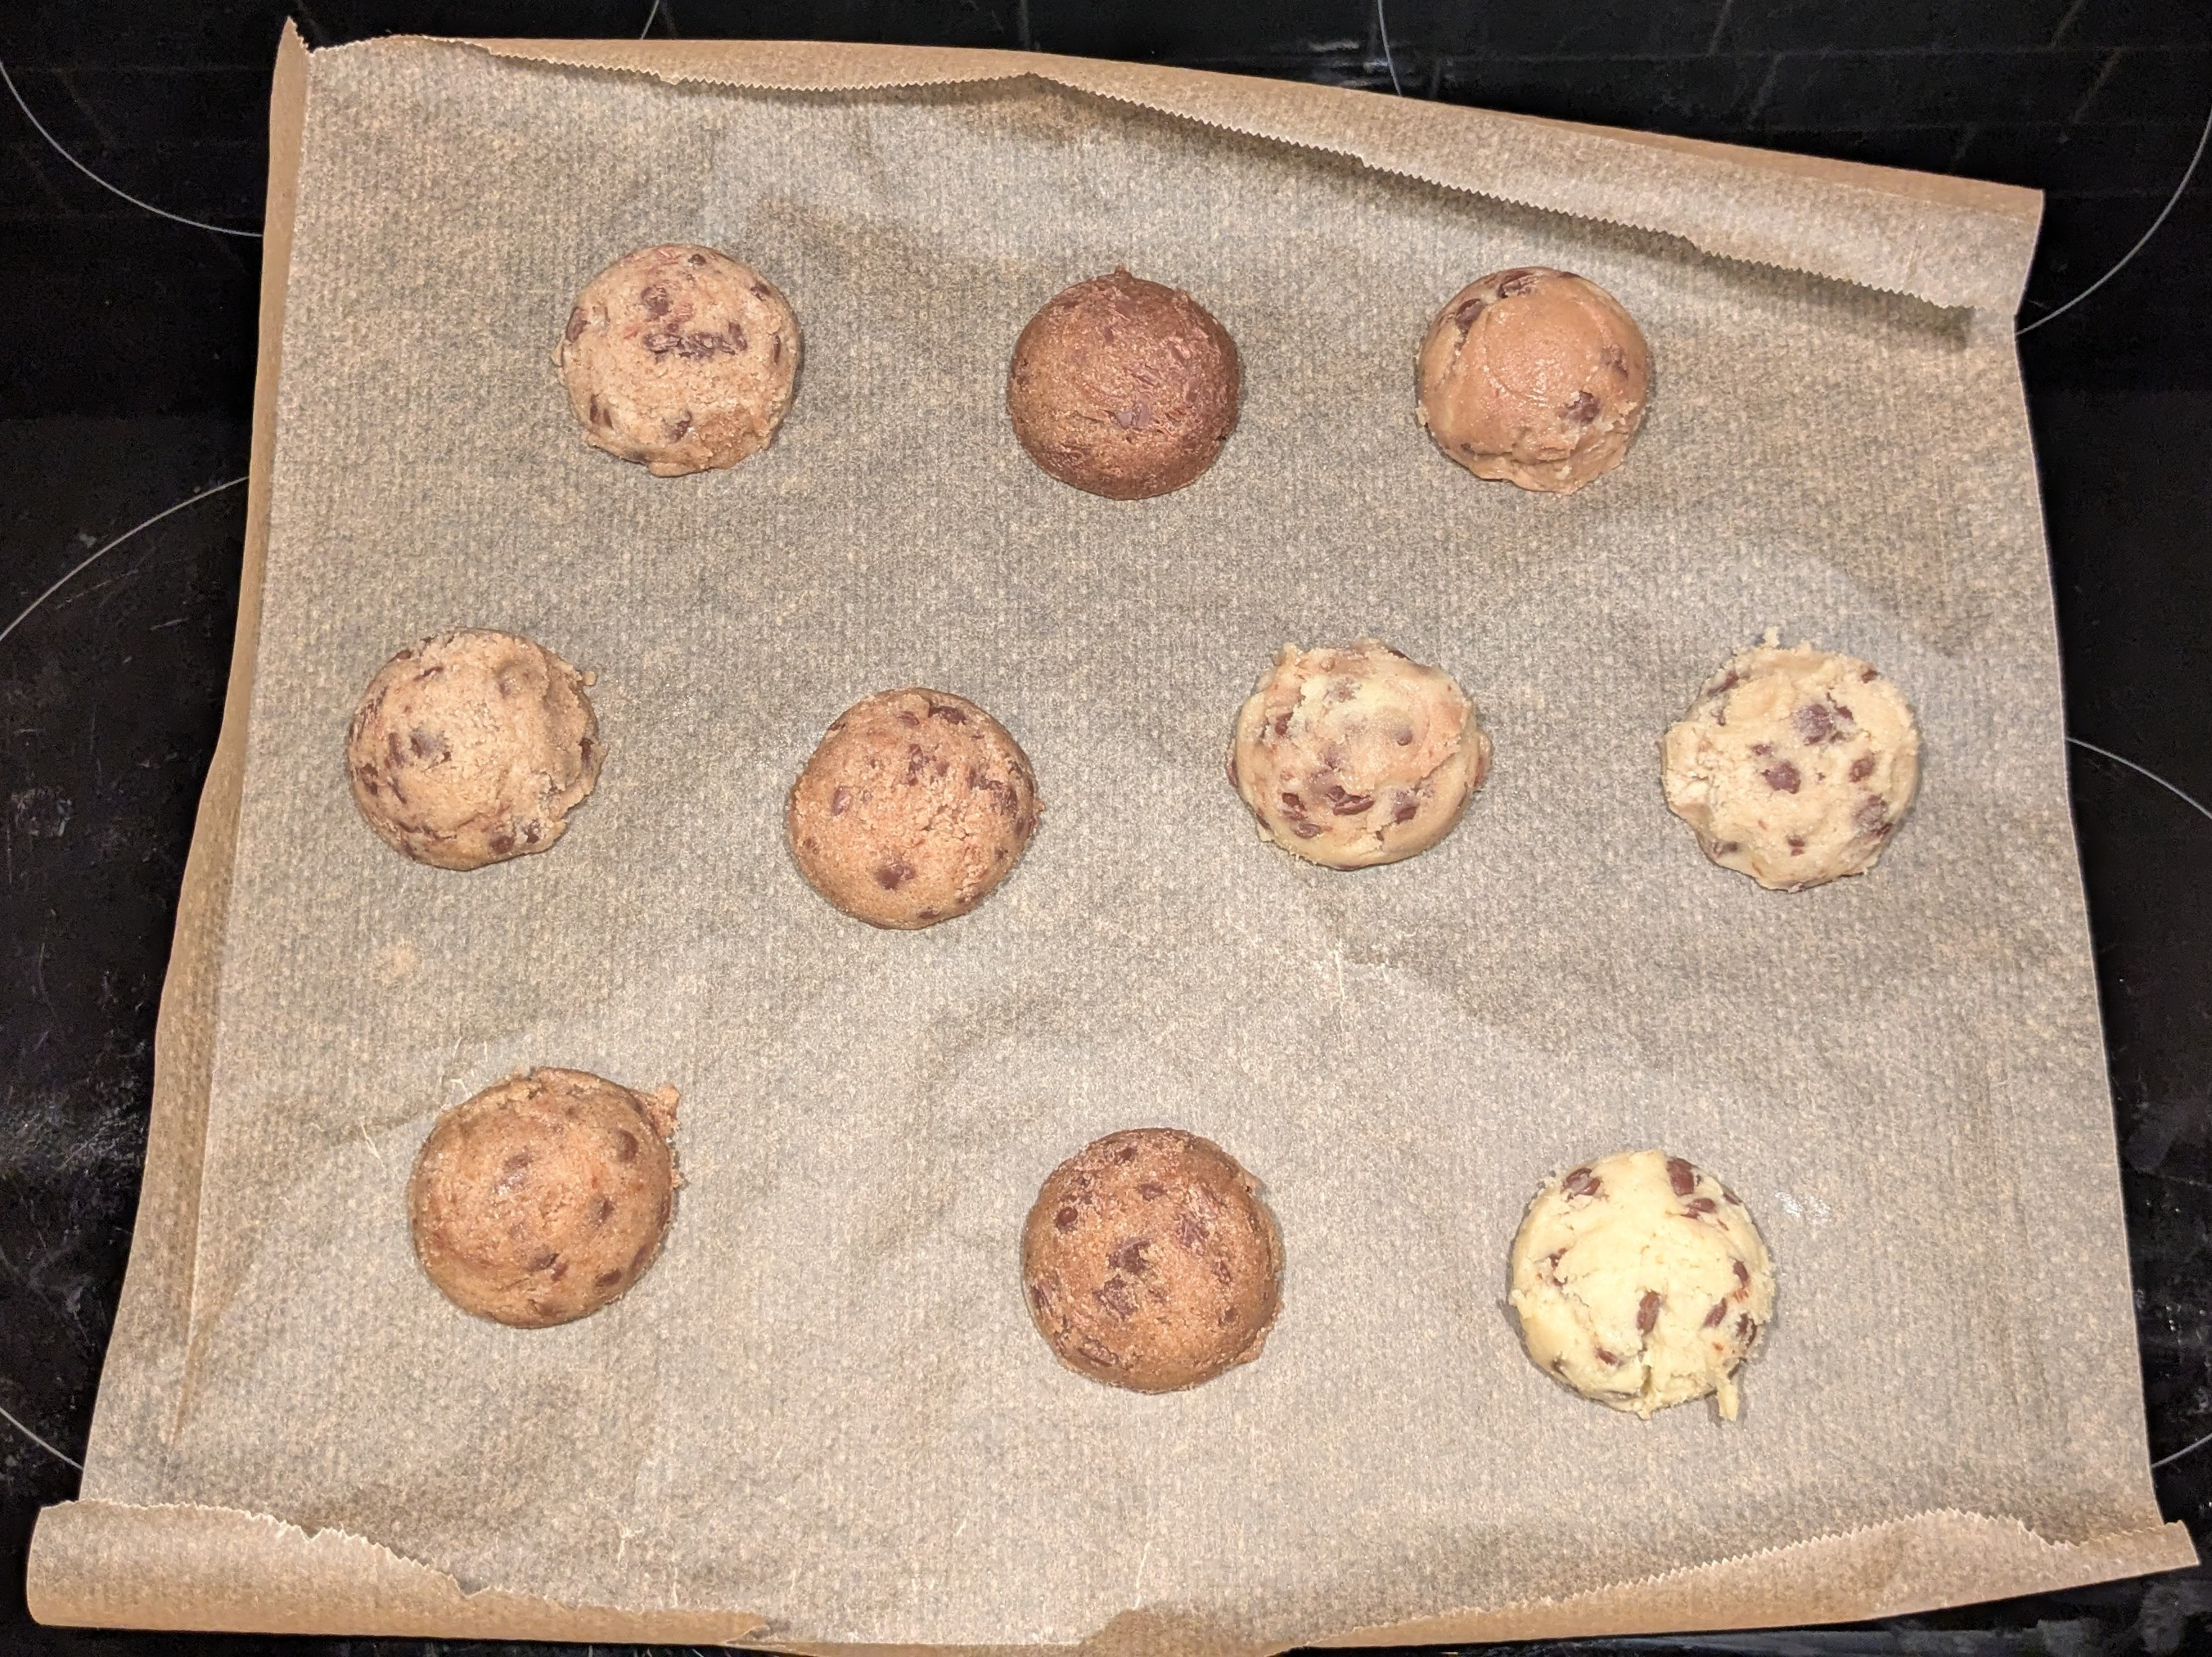
\includegraphics[width = \textwidth]{figures/block2_1_vorher.jpg}
\caption{Teigrohlinge vor dem Backen}
\label{fig:block2_1_vorher}
\end{subfigure}\hfill
\begin{subfigure}{0.49\textwidth}
\centering
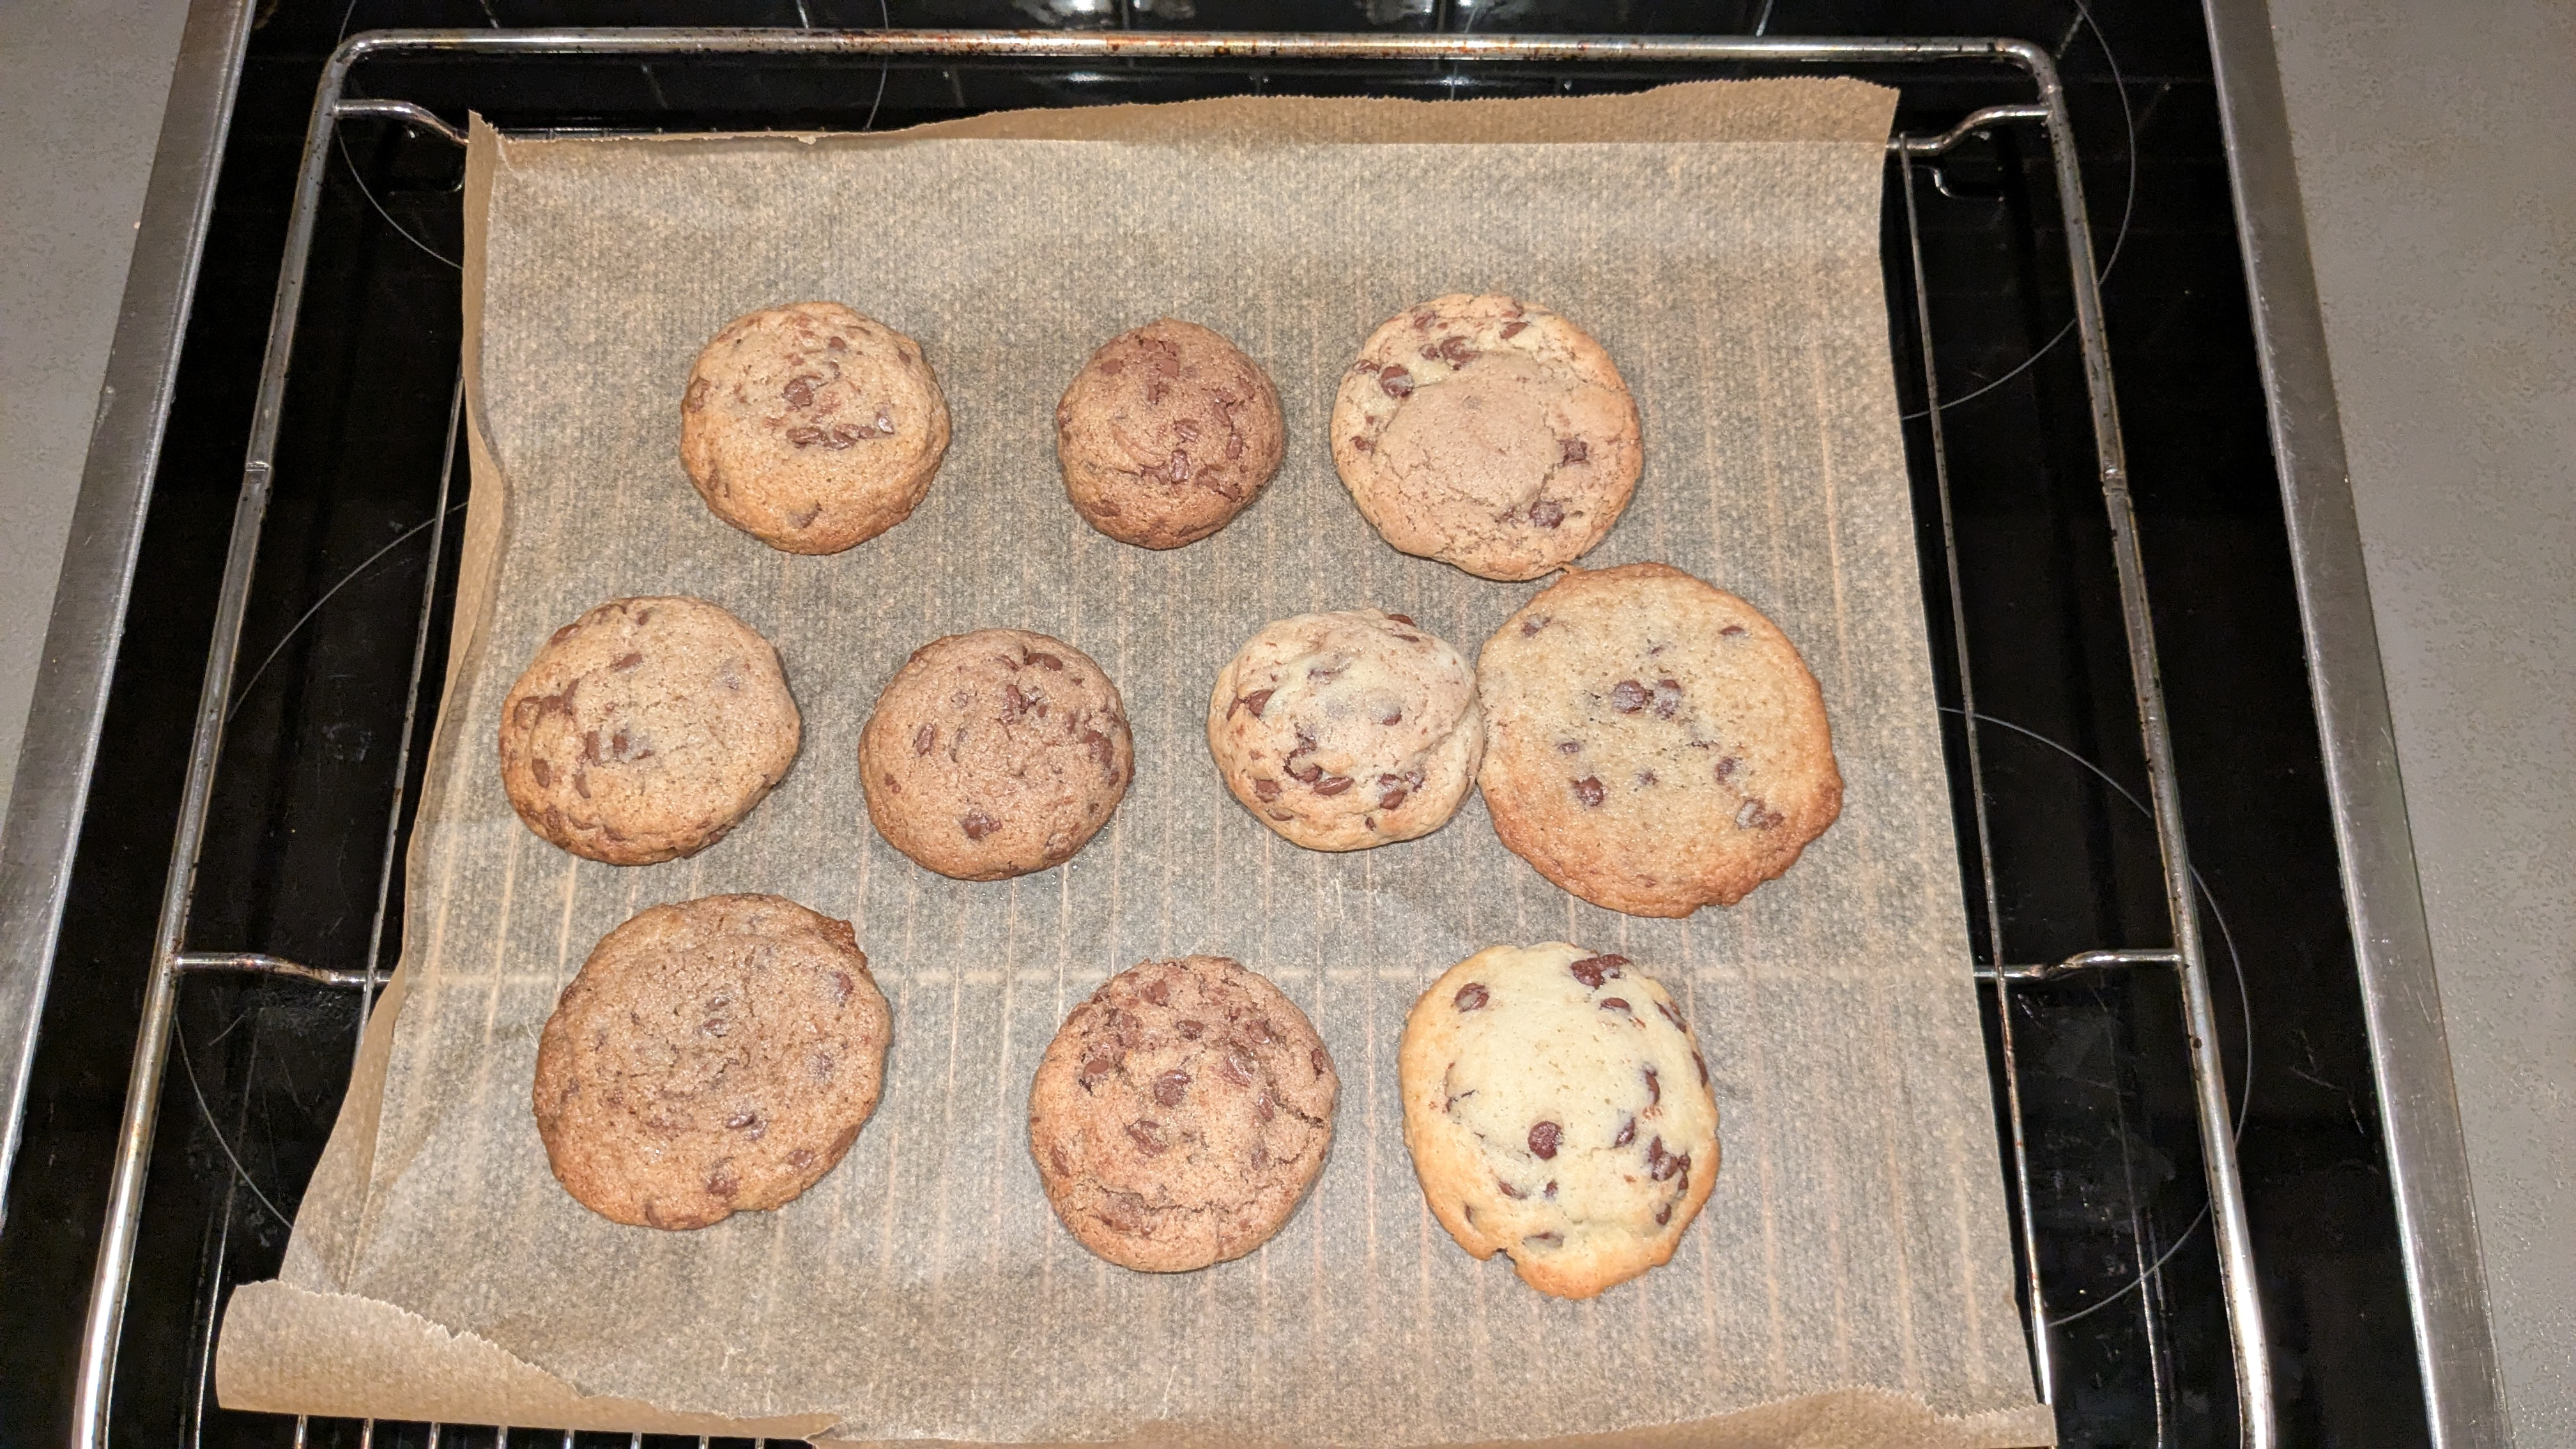
\includegraphics[width = \textwidth]{figures/block2_3_nachher.jpg}
\caption{Cookies nach dem Backvorgang}
\label{fig:block2_3_nacher}
\end{subfigure}

\caption{Backvorgang der zweiten Replikation}
\label{fig:block_2}
\end{figure}

\begin{figure}
\centering
\begin{subfigure}{0.49\textwidth}
\centering
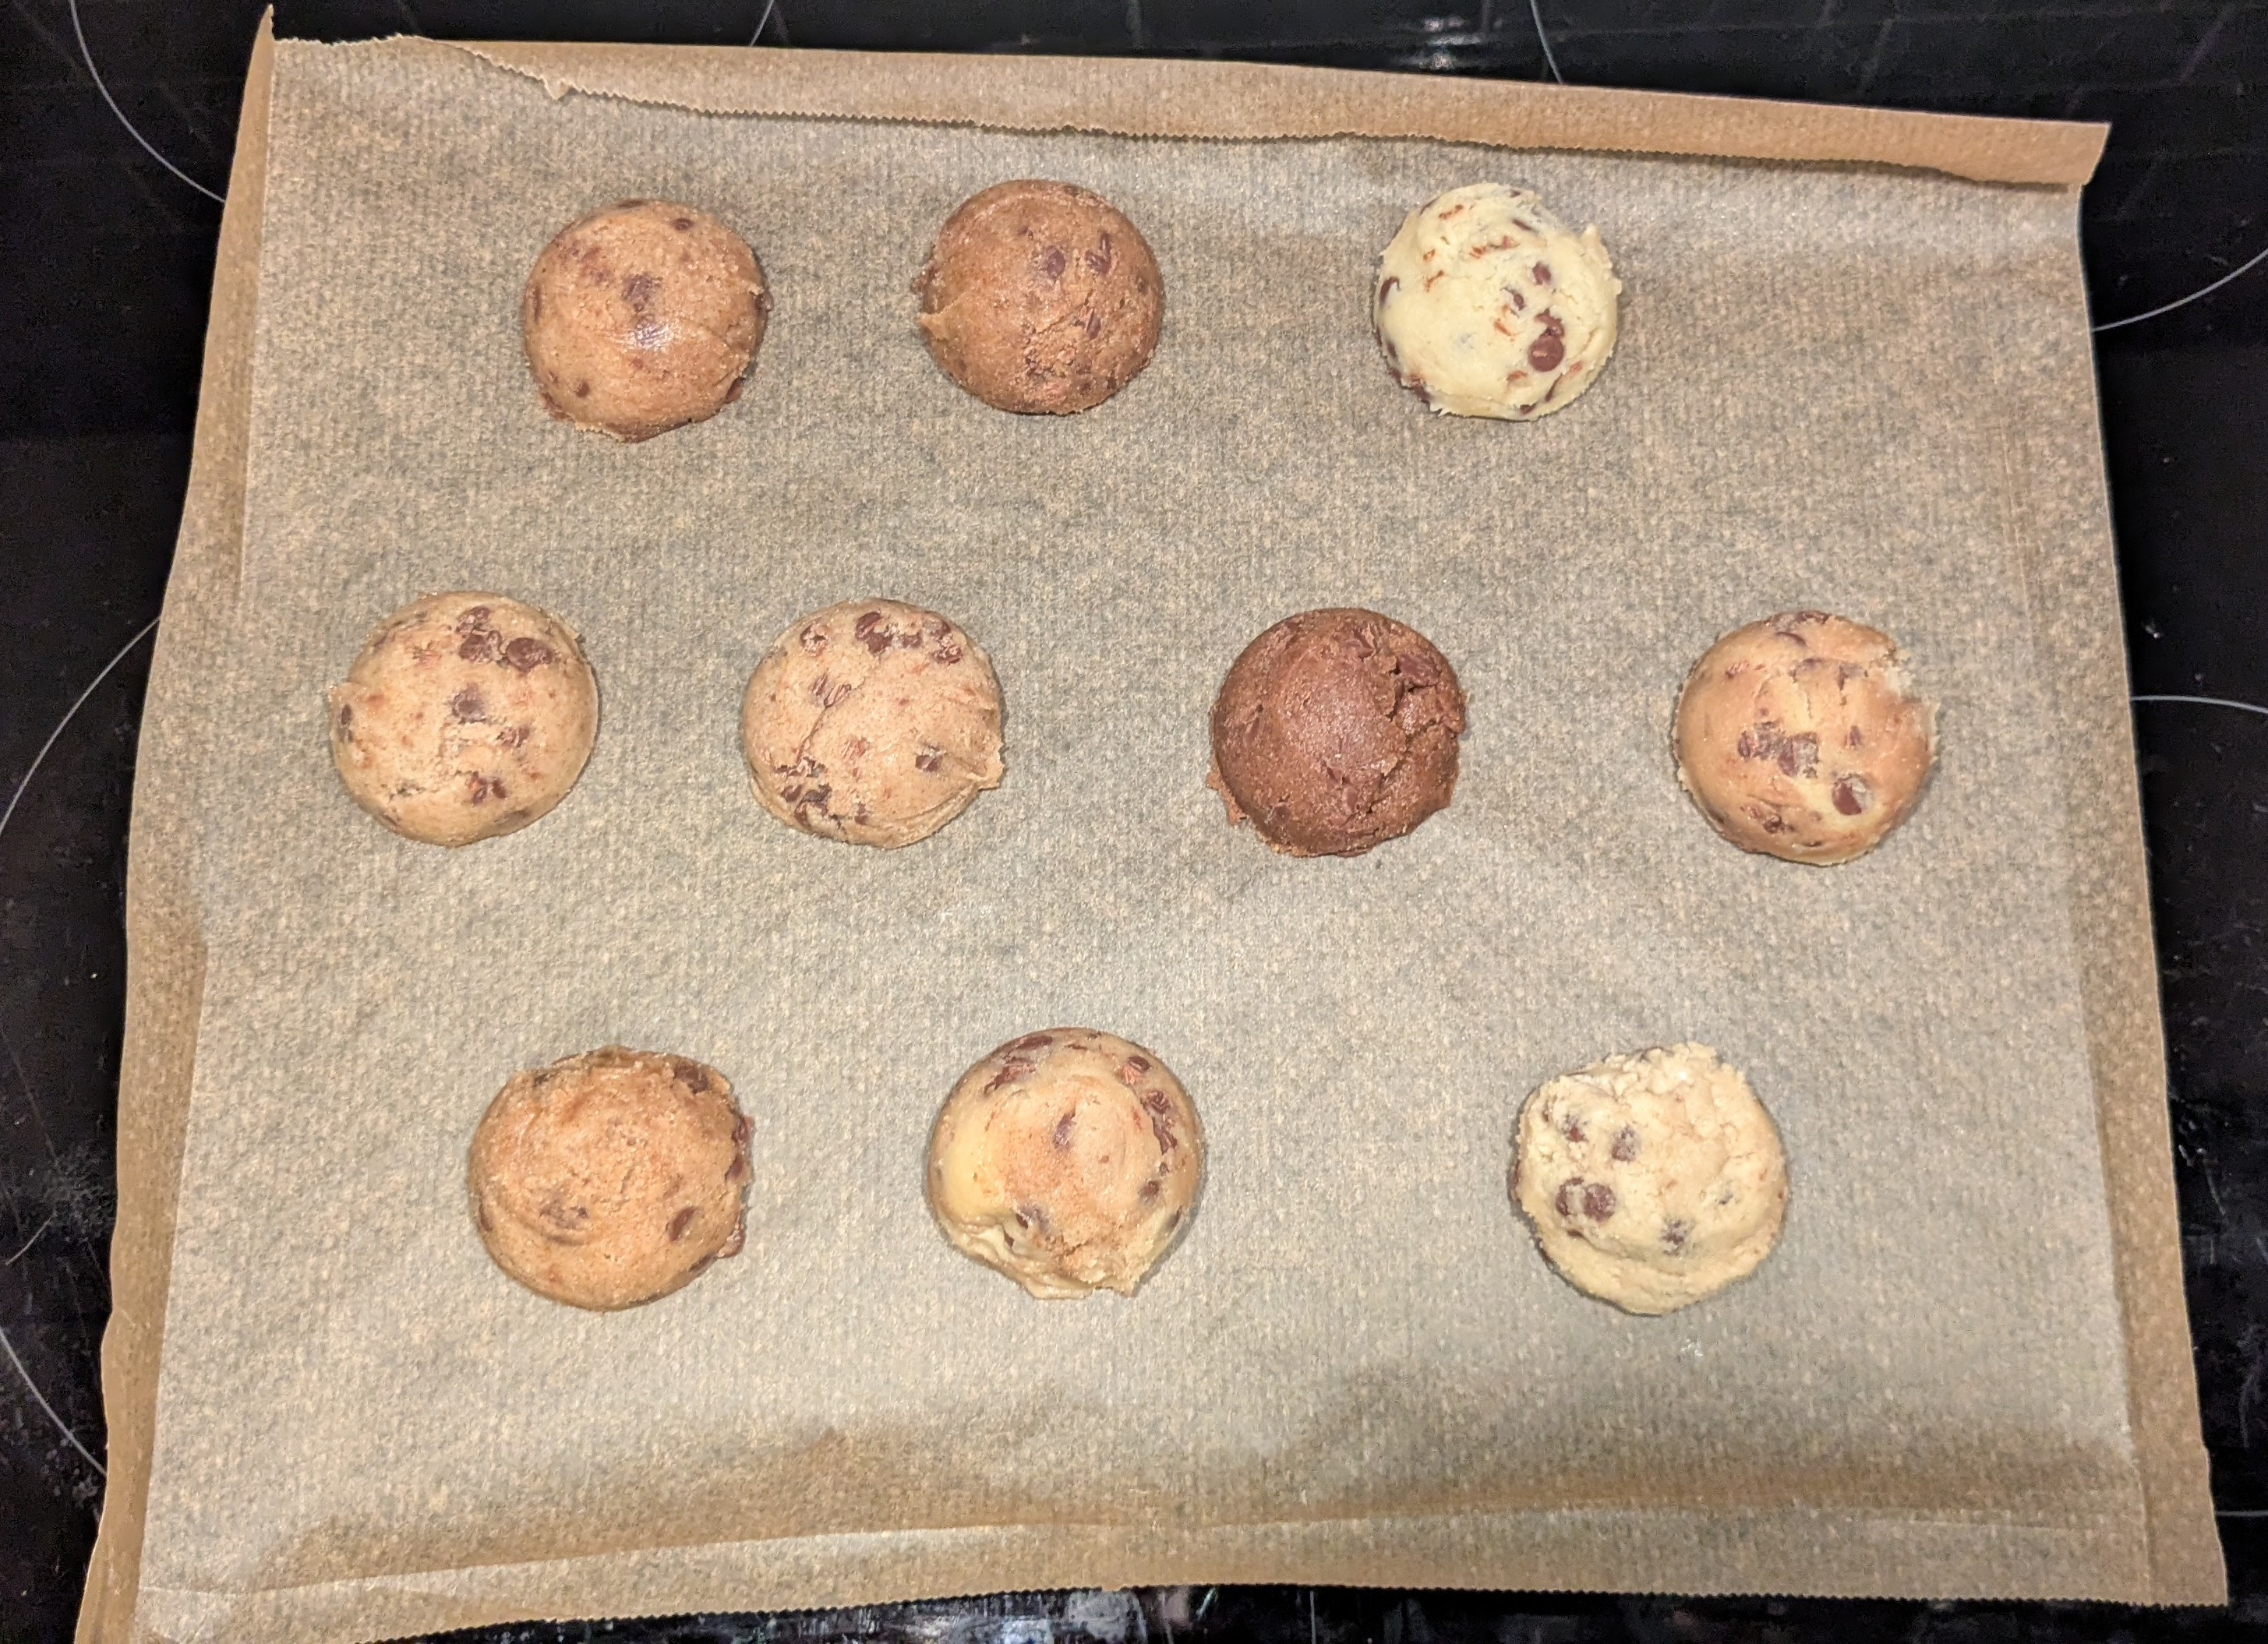
\includegraphics[width = \textwidth]{figures/block3_1_vorher.jpg}
\caption{Teigrohlinge vor dem Backen}
\label{fig:block3_1_vorher}
\end{subfigure}\hfill
\begin{subfigure}{0.49\textwidth}
\centering
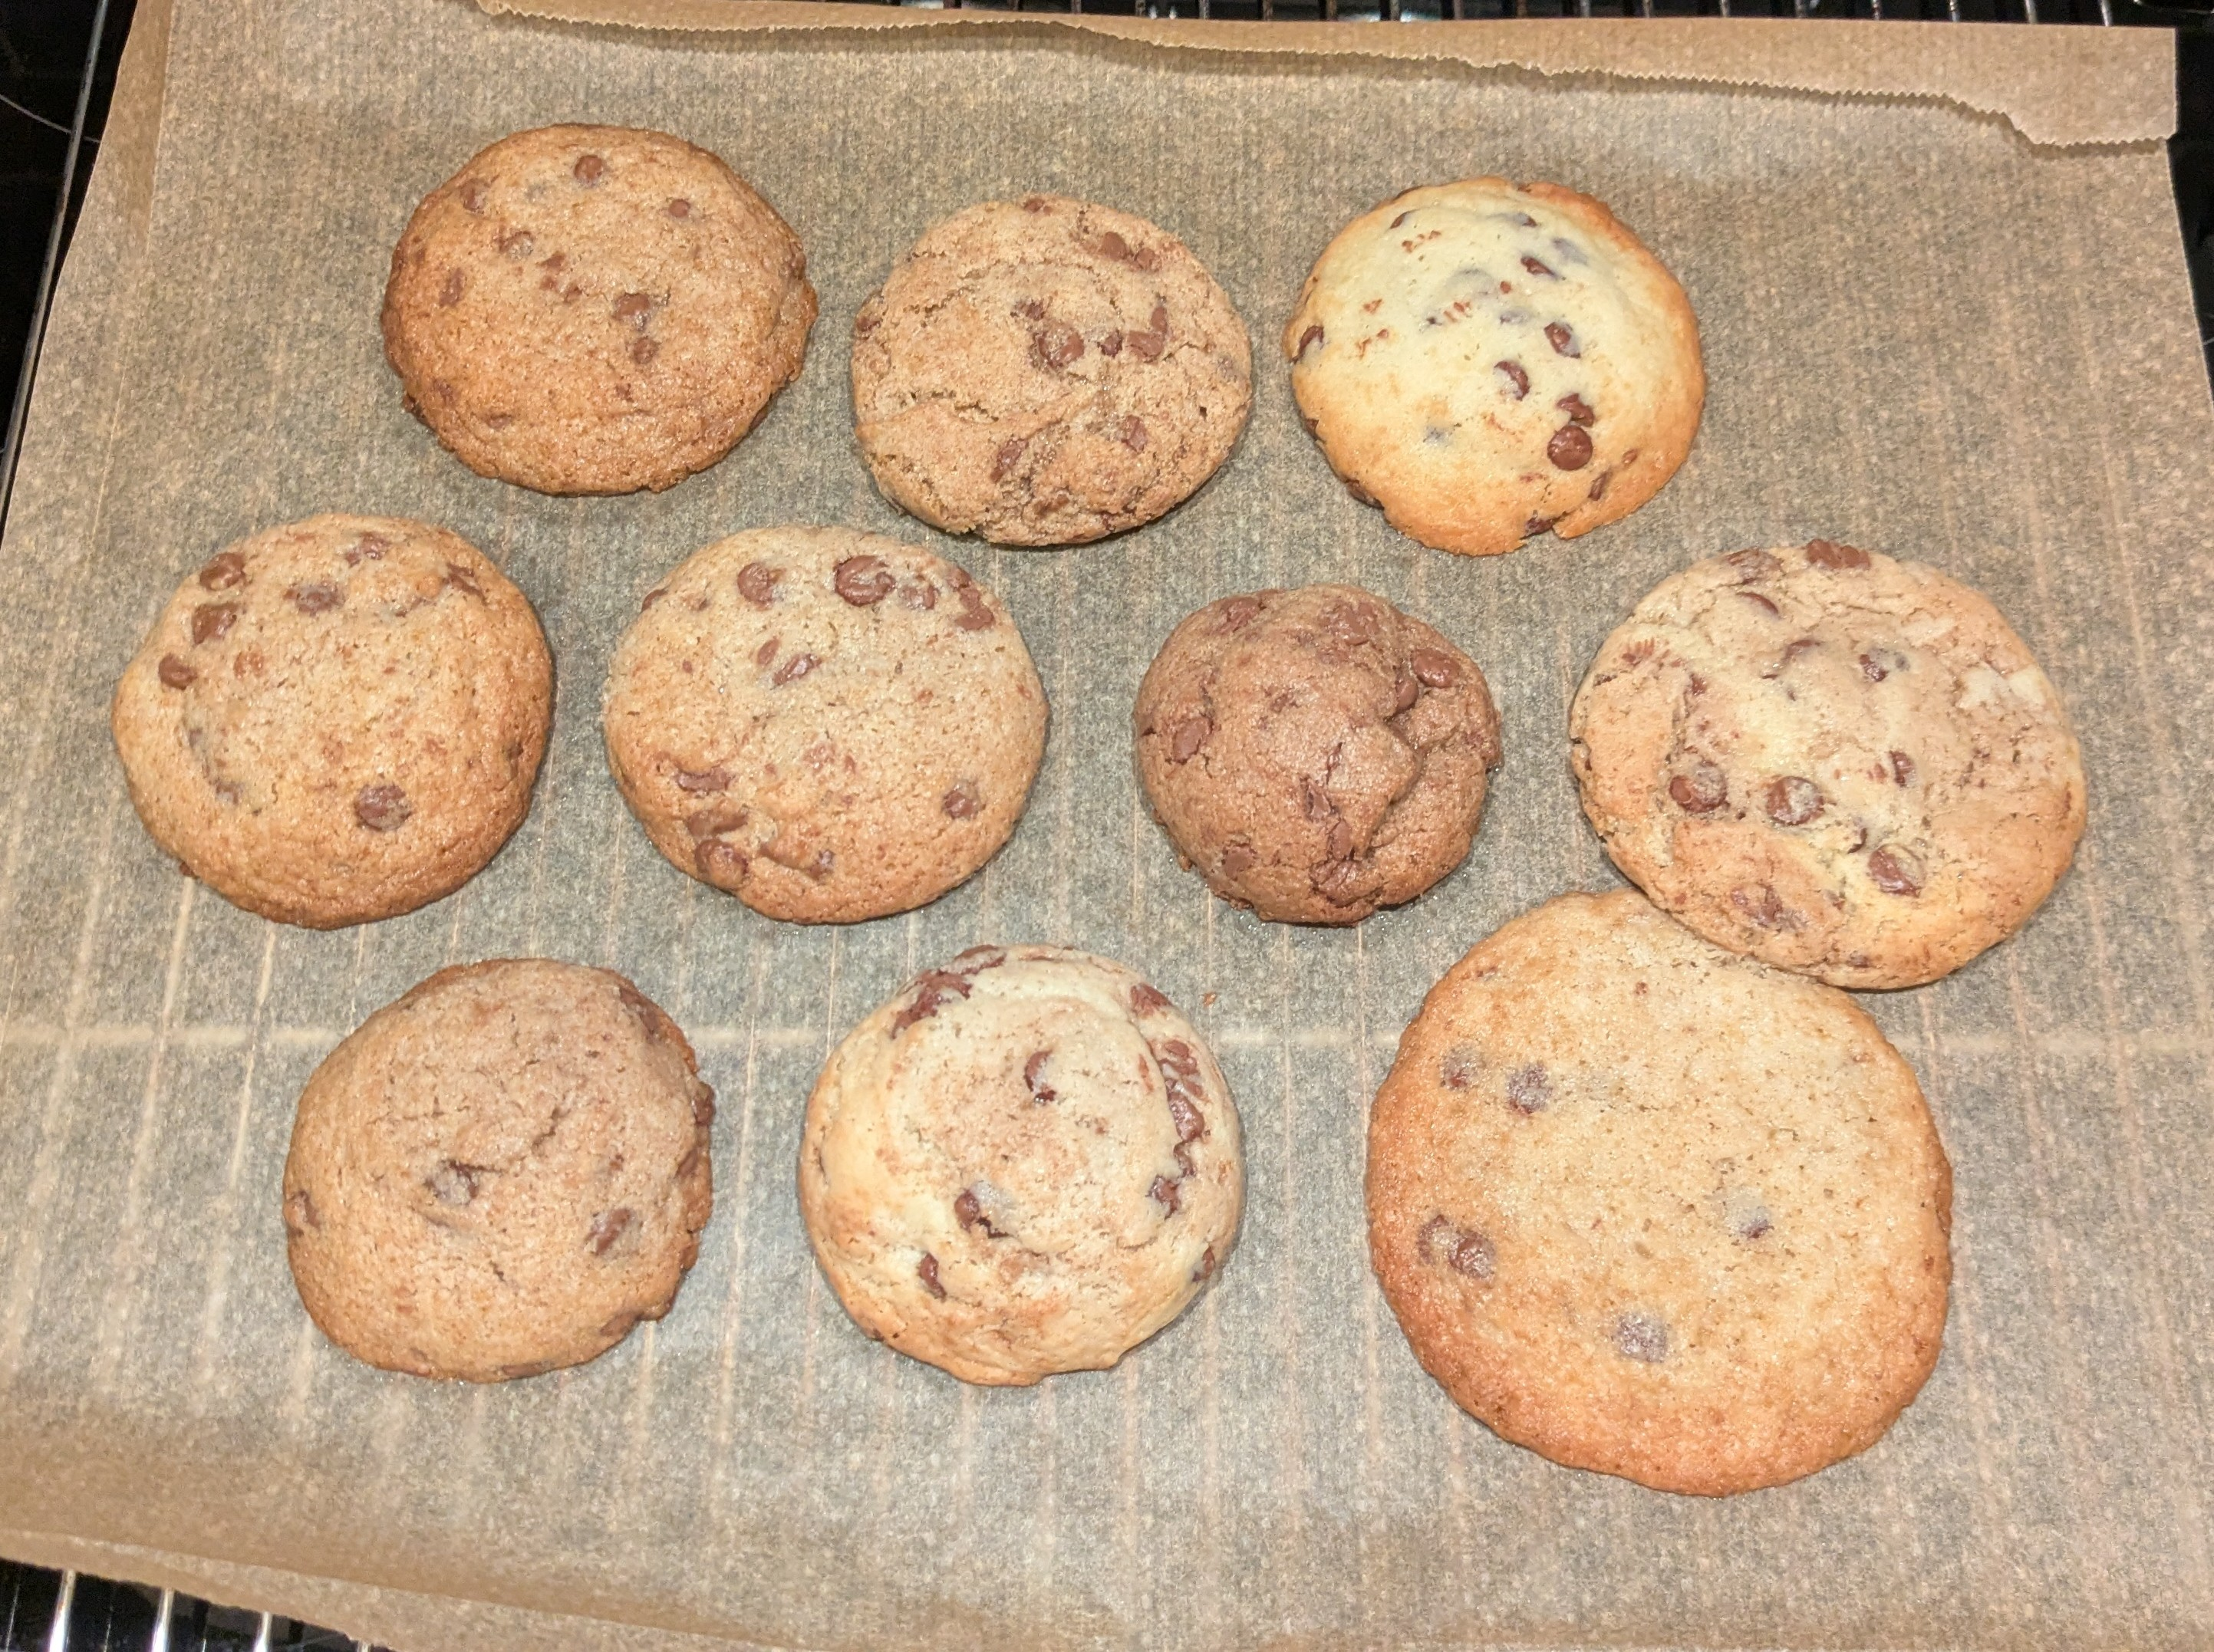
\includegraphics[width = \textwidth]{figures/block3_4_nachher.jpg}
\caption{Cookies nach dem Backvorgang}
\label{fig:block3_4_nacher}
\end{subfigure}
\caption{Backvorgang der dritten Replikation}
\label{fig:block_3}
\end{figure}  % Appendix content

\end{document}